\documentclass[11pt,a4paper]{article}
\usepackage[utf8]{inputenc}
\usepackage[T1]{fontenc}
\usepackage[spanish,es-noshorthands,es-tabla,es-nodecimaldot]{babel}
\usepackage{lmodern}

\usepackage[a4paper,top=1.8cm,bottom=1.8cm,left=1.8cm,right=1.8cm,
            headheight=22pt,footskip=0.8cm]{geometry}

\usepackage{amsmath,amssymb}
\usepackage{bm}
\usepackage{graphicx}
\usepackage{xcolor}
\usepackage{booktabs}
\usepackage{tabularx}
\usepackage{array}
\usepackage{ragged2e}
\usepackage{enumitem}
\usepackage{fancyhdr}
\usepackage{titlesec}
\usepackage{listings}
\usepackage[most]{tcolorbox}
\usepackage{hyperref}
\usepackage[section]{placeins}
\usepackage{needspace}

% Optimización de colocación de flotantes para evitar páginas vacías
\renewcommand{\topfraction}{0.90}
\renewcommand{\bottomfraction}{0.90}
\renewcommand{\textfraction}{0.10}
\renewcommand{\floatpagefraction}{0.75}
\setlength{\floatsep}{4pt plus 1pt minus 1pt}
\setlength{\textfloatsep}{6pt plus 1pt minus 1pt}
\setlength{\intextsep}{4pt plus 1pt minus 1pt}

\definecolor{navy}{HTML}{1E2761}
\definecolor{coral}{HTML}{F96167}
\definecolor{iceblue}{HTML}{CADCFC}
\definecolor{grisclaro}{HTML}{F4F6FB}

\hypersetup{
  colorlinks=true,
  linkcolor=navy,
  urlcolor=coral,
  citecolor=navy,
  pdftitle={Laboratorio Dirigido Nro. 2 - Logica CMOS Dinamica},
  pdfauthor={Leonardo Yactayo Tolentino, Marco Arcila Santander - UNMSM FIEE}
}

% -------------------------------- Encabezados ----------------------------------
\pagestyle{fancy}
\fancyhf{}
\fancyhead[L]{\footnotesize\color{navy}\textsc{Microelectrónica y Sistemas Nanoelectrónicos} · Laboratorio N.\textsuperscript{o} 2}
\fancyhead[R]{\footnotesize\color{navy}LD2 -- Lógica CMOS Dinámica}
\fancyfoot[L]{\footnotesize\color{navy}MsC. Luz Adanaqué Infante}
\fancyfoot[C]{\footnotesize\color{navy}UNMSM -- FIEE}
\fancyfoot[R]{\footnotesize\color{navy}\thepage}
\renewcommand{\headrulewidth}{0.8pt}
\renewcommand{\footrulewidth}{0.4pt}
\renewcommand{\headrule}{\hbox to\headwidth{\color{coral}\leaders\hrule height \headrulewidth\hfill}}

% -------------------------------- Titulos --------------------------------------
\titleformat{\section}
  {\normalfont\Large\bfseries\color{navy}}{\thesection.}{0.6em}{}
  [\vspace{-0.6em}{\color{coral}\rule{\textwidth}{1.2pt}}]
\titleformat{\subsection}
  {\normalfont\large\bfseries\color{navy}}{\thesubsection}{0.6em}{}
\titleformat{\subsubsection}
  {\normalfont\normalsize\bfseries\color{navy}}{\thesubsubsection}{0.5em}{}
\titlespacing*{\section}{0pt}{1.0em}{0.4em}
\titlespacing*{\subsection}{0pt}{0.7em}{0.3em}
\titlespacing*{\subsubsection}{0pt}{0.5em}{0.2em}

% --------------------------- Estilo para codigo SPICE --------------------------
\lstdefinelanguage{SPICE}{
  alsoletter={.},
  morekeywords={.include,.param,.model,.tran,.dc,.ac,.op,.meas,.measure,.step,
                .ic,.subckt,.ends,.end,.options,.lib,.save,.four,
                PULSE,PWL,SIN,TRIG,TARG,VAL,RISE,FALL,TD,AVG,MAX,MIN,PARAM,
                FIND,WHEN,AT,DERIV,nmos,pmos,level},
  sensitive=false,
  morecomment=[f]{*},
  morecomment=[l]{;},
}
\lstdefinestyle{spice}{
  language=SPICE,
  basicstyle=\fontsize{7.5pt}{8.8pt}\selectfont\ttfamily,
  keywordstyle=\color{navy}\bfseries,
  commentstyle=\color{coral!85!black}\itshape,
  backgroundcolor=\color{grisclaro},
  frame=leftline,
  framerule=1.5pt,
  rulecolor=\color{iceblue},
  framesep=4pt,
  xleftmargin=6pt,
  breaklines=true,
  showstringspaces=false,
  columns=fullflexible,
  aboveskip=0.6em,
  belowskip=0.6em,
}
\lstset{style=spice}

% --------------------------------- Cajas ---------------------------------------
\newtcolorbox{aviso}[1][]{
  enhanced, breakable, colback=coral!8, colframe=coral,
  boxrule=0pt, leftrule=3.5pt, arc=2pt, left=8pt, right=8pt, top=6pt, bottom=6pt,
  fonttitle=\bfseries\color{white}, #1}

\newtcolorbox{nota}[1][]{
  enhanced, breakable, colback=iceblue!35, colframe=navy,
  boxrule=0pt, leftrule=3.5pt, arc=2pt, left=8pt, right=8pt, top=6pt, bottom=6pt,
  #1}

\newtcolorbox{preguntas}[1][]{
  enhanced, breakable, colback=white, colframe=navy,
  boxrule=0.8pt, arc=2pt, left=6pt, right=6pt, top=4pt, bottom=4pt,
  title={\bfseries #1}, coltitle=white, colbacktitle=navy}

% ---------------------------- Utilidades y Tablas -----------------------------
\renewcommand{\arraystretch}{1.20}
\setlength{\tabcolsep}{4pt}

% ==============================================================================
\begin{document}
% ==============================================================================

% --------------------------------- Portada ------------------------------------
\hypersetup{pageanchor=false}
\begin{titlepage}
\centering
\vspace*{1.0cm}

{\color{navy}\rule{\textwidth}{2pt}}\\[0.5em]
{\Large\bfseries\color{navy} UNIVERSIDAD NACIONAL MAYOR DE SAN MARCOS}\\[0.35em]
{\normalsize\color{navy} Universidad del Perú, Decana de América}\\[0.6em]
{\color{coral}\rule{\textwidth}{2pt}}\\[1.2cm]

{\large\color{navy} Facultad de Ingeniería Electrónica y Eléctrica}\\[0.3em]
{\large\color{navy} Escuela Profesional de Ingeniería Electrónica}\\[1.8cm]

{\color{coral}\Large\bfseries INFORME DE LABORATORIO DIRIGIDO N.\textsuperscript{o} 2}\\[0.8cm]
{\Huge\bfseries\color{navy} Lógica CMOS Dinámica}\\[0.7cm]
{\large\color{navy}\itshape Caracterización Temporal, Robustez frente a Fugas,\\ Métricas de Consumo y Dimensionamiento en Tecnologías Submicrométricas}\\[2.0cm]

\begin{tabular}{@{}r@{\hspace{1em}}l@{}}
\bfseries\color{navy} Curso: & Microelectrónica y Sistemas Nanoelectrónicos (Semestre 2026-II) \\
\bfseries\color{navy} Docente: & MsC. Luz Adanaqué Infante \\
\bfseries\color{navy} Integrantes: & Leonardo Sait Yactayo Tolentino (23190214) \\
                                   & Marco Antonio Arcila Santander (23190140) \\
\bfseries\color{navy} Modalidad: & Parejas \\
\end{tabular}

\vfill
{\color{iceblue}\rule{\textwidth}{6pt}}\\[0.4em]
{\footnotesize\color{navy} Lima, Perú --- 2026}
\end{titlepage}

\newpage
\hypersetup{pageanchor=true}
\pagenumbering{arabic}

% --------------------------------- Contenido ----------------------------------
% ==============================================================================
% SECCION 1: METODOLOGIA Y ENTORNO DE SIMULACION FISICA
% ==============================================================================
\section{Metodología y Configuración del Entorno de Simulación}
\label{sec:metodologia}

Para el desarrollo del presente informe se implementó una infraestructura de simulación automatizada en SPICE y post-procesamiento en Python, orientada a garantizar reproducibilidad determinística y trazabilidad física absoluta en cada ensayo.

\subsection{Modelos de Dispositivos y Nodo Tecnológico}
Se emplean tarjetas de modelo predictivas BSIM4 (\textit{Predictive Technology Model}, PTM) desarrolladas por la Universidad Estatal de Arizona (ASU / Nanoscale Integration and Modeling Group). Con el propósito de prevenir colisiones de nombres al incluir múltiples nodos en simulaciones de referencia cruzada, los modelos se integraron en librerías modulares:
\begin{itemize}[leftmargin=1.4em,itemsep=0.1em]
  \item \texttt{ptm45hp.lib}: Proceso PTM de 45\,nm \textit{High Performance} ($V_{DD} = 1.0\,\text{V}$, $L_{\text{nom}} = 45\,\text{nm}$, $t_{oxe} = 1.25\,\text{nm}$, $V_{th0,n} \approx 0.47\,\text{V}$, $V_{th0,p} \approx -0.42\,\text{V}$). Nodo primario en la Actividad~1.
  \item \texttt{ptm45lp.lib}: Proceso PTM de 45\,nm \textit{Low Power} ($V_{DD} = 1.1\,\text{V}$, $L_{\text{nom}} = 45\,\text{nm}$, $t_{oxe} = 1.80\,\text{nm}$, $V_{th0,n} \approx 0.62\,\text{V}$, $V_{th0,p} \approx -0.58\,\text{V}$).
  \item \texttt{ptm130.lib}: Proceso clásico de 130\,nm Bulk ($V_{DD} = 1.3\,\text{V}$, $L_{\text{nom}} = 130\,\text{nm}$, $t_{oxe} = 3.10\,\text{nm}$).
\end{itemize}

\subsection{Parámetros Numéricos del Solver SPICE}
De acuerdo con las directrices de diseño submicrométrico para lógica dinámica, se estableció como directiva mandatoria en todos los archivos de netlist (\texttt{.cir}):
\begin{lstlisting}[style=spice]
.options gmin=1e-15 abstol=1e-14 reltol=1e-4 method=gear
\end{lstlisting}

La selección de estos parámetros responde a requerimientos físicos concretos:
\begin{enumerate}[leftmargin=1.4em,itemsep=0.12em]
  \item \textbf{Conductancia de regularización (\texttt{gmin = 1e-15}):} El valor predeterminado de LTspice (\texttt{gmin = 1e-12}, correspondiente a $1\,\text{pS}$) conecta una conductancia parásita hacia tierra en cada nodo, inyectando una corriente artificial calculable como $I_{gmin} = G_{min} \cdot V_{DD} = 10^{-12} \times 1.0\,\text{V} = 1.0\,\text{pA}$. En transistores de 45\,nm en estado de reposo, esta corriente numérica es comparable a las fugas físicas subumbral, distorsionando severamente las evaluaciones de retención de carga en nodos flotantes. Reducir \texttt{gmin} a $1\,\text{fS}$ minimiza esta inyección espuria a $1.0\,\text{aA}$ ($10^{-18}\,\text{A}$).
  \item \textbf{Tolerancias de convergencia (\texttt{abstol = 1e-14}, \texttt{reltol = 1e-4}):} Las corrientes residuales subumbral y de túnel en dispositivos en corte se ubican en el rango de femtoamperios. La tolerancia estándar ($10^{-12}\,\text{A}$) induce ruido numérico y falsas oscilaciones durante la evaluación de nodos dinámicos.
  \item \textbf{Algoritmo de integración (\texttt{method = gear}):} El método trapezoidal estándar (\texttt{trap}) produce resonancias numéricas artificiales (\textit{trapezoidal ringing}) cuando ocurren transiciones de tensión con tiempos de subida extremadamente reducidos ($t_r = 20\,\text{ps}$) sobre nodos con capacitancias parásitas de femtofaradios. La integración de Gear proporciona un amortiguamiento numérico incondicional sin alterar la constante de tiempo física $RC$.
\end{enumerate}

\subsection{Flujo de Extracción y Trazabilidad}
Todas las simulaciones fueron procesadas en modo \textit{batch} silencioso (\texttt{-b}) mediante LTspice v26.0.2 bajo Windows. Las figuras fueron generadas directamente a partir de los datos crudos extraídos de los ficheros \texttt{.raw} a 300\,DPI en formato matricial con ejes normalizados, mientras que las métricas escalares fueron recolectadas de los ficheros \texttt{.log} mediante directivas \texttt{.meas} acotadas en tiempo y un parser automatizado de regresión.

% ==============================================================================
% SECCION 2: ACTIVIDAD 1 - NAND3 DINAMICA FOOTED
% ==============================================================================
\needspace{6\baselineskip}
\section{Actividad 1: NAND3 CMOS Dinámica Footed (Fases, Asimetría y Consumo)}
\label{sec:actividad1}

\subsection{Topología Circuital y Dimensionamiento}
La compuerta NAND3 dinámica analizada se implementa en configuración \textit{footed} complementada por un inversor dominó restaurador, operando bajo tecnología PTM de 45\,nm HP ($V_{DD} = 1.0\,\text{V}$, $T = 27^\circ\text{C}$). 

\begin{itemize}[leftmargin=1.4em,itemsep=0.15em]
  \item \textbf{Red de Descarga (PDN) y Footer ($M_f$):} Cuatro transistores NMOS en serie ($M_1, M_2, M_3$ para las entradas lógicas $A, B, C$, y $M_f$ para $CLK$). Los tres NMOS lógicos y el footer adoptan $W_n = 3 \times 90\,\text{nm} = 270\,\text{nm}$ ($L = 45\,\text{nm}$); la aproximación geométrica de cuatro dispositivos en serie establece una anchura efectiva de $W_{PDN,eq} = 270\,\text{nm}/4 = 67.5\,\text{nm}$ (consistente con el modelado de contención en la Actividad~3), en lugar de equiparar exactamente a un NMOS unitario de $90\,\text{nm}$.
  \item \textbf{Transistor de Precarga ($M_p$):} Dispositivo PMOS ($W_p = 135\,\text{nm}$, $L = 45\,\text{nm}$) conectado a $V_{DD}$, gobernado por $CLK$ en nivel bajo ($\beta = 1.5$ respecto al NMOS de $90\,\text{nm}$).
  \item \textbf{Inversor Dominó de Salida:} Etapa restauradora no inversora con $M_{pi}$ ($W_p = 135\,\text{nm}$) y $M_{ni}$ ($W_n = 90\,\text{nm}$).
  \item \textbf{Condiciones de Carga:} Capacitancia concentrada explícita $C_L = 2\,\text{fF}$ en el nodo interno $dyn$ y capacitancia de carga $C_{out} = 1\,\text{fF}$ en el terminal de salida $out$.
  \item \textbf{NAND3 CMOS Estática Equivalente:} PUN de 3 PMOS en paralelo ($W_p = 135\,\text{nm}$) y PDN de 3 NMOS en serie ($W_n = 270\,\text{nm}$), con carga idéntica $C_{out} = 1\,\text{fF}$.
\end{itemize}

Estructuralmente, el núcleo dinámico \textit{footed} requiere únicamente 5 transistores (4 NMOS + 1 PMOS) y 7 transistores con la etapa dominó completa, frente a los 6 transistores requeridos por la NAND3 estática convencional.

\subsection{Análisis Temporal y Fases de Operación}
Para caracterizar el ciclo secuencial, se aplicó reloj a $500\,\text{MHz}$ ($T_{clk} = 2.0\,\text{ns}$, ciclo de trabajo del 50\%) y un estímulo de entrada $A$ a $125\,\text{MHz}$ ($T_A = 8.0\,\text{ns}$) con retardo de $t_{\text{delay}} = 1.1\,\text{ns}$ ($0.55\,T_{clk}$), fijando $B=C=V_{DD}$. Las curvas se ilustran en la Figura~\ref{fig:fases_formas_onda}, distinguiéndose las cuatro fases operativas:

\begin{figure}[htbp]
  \centering
  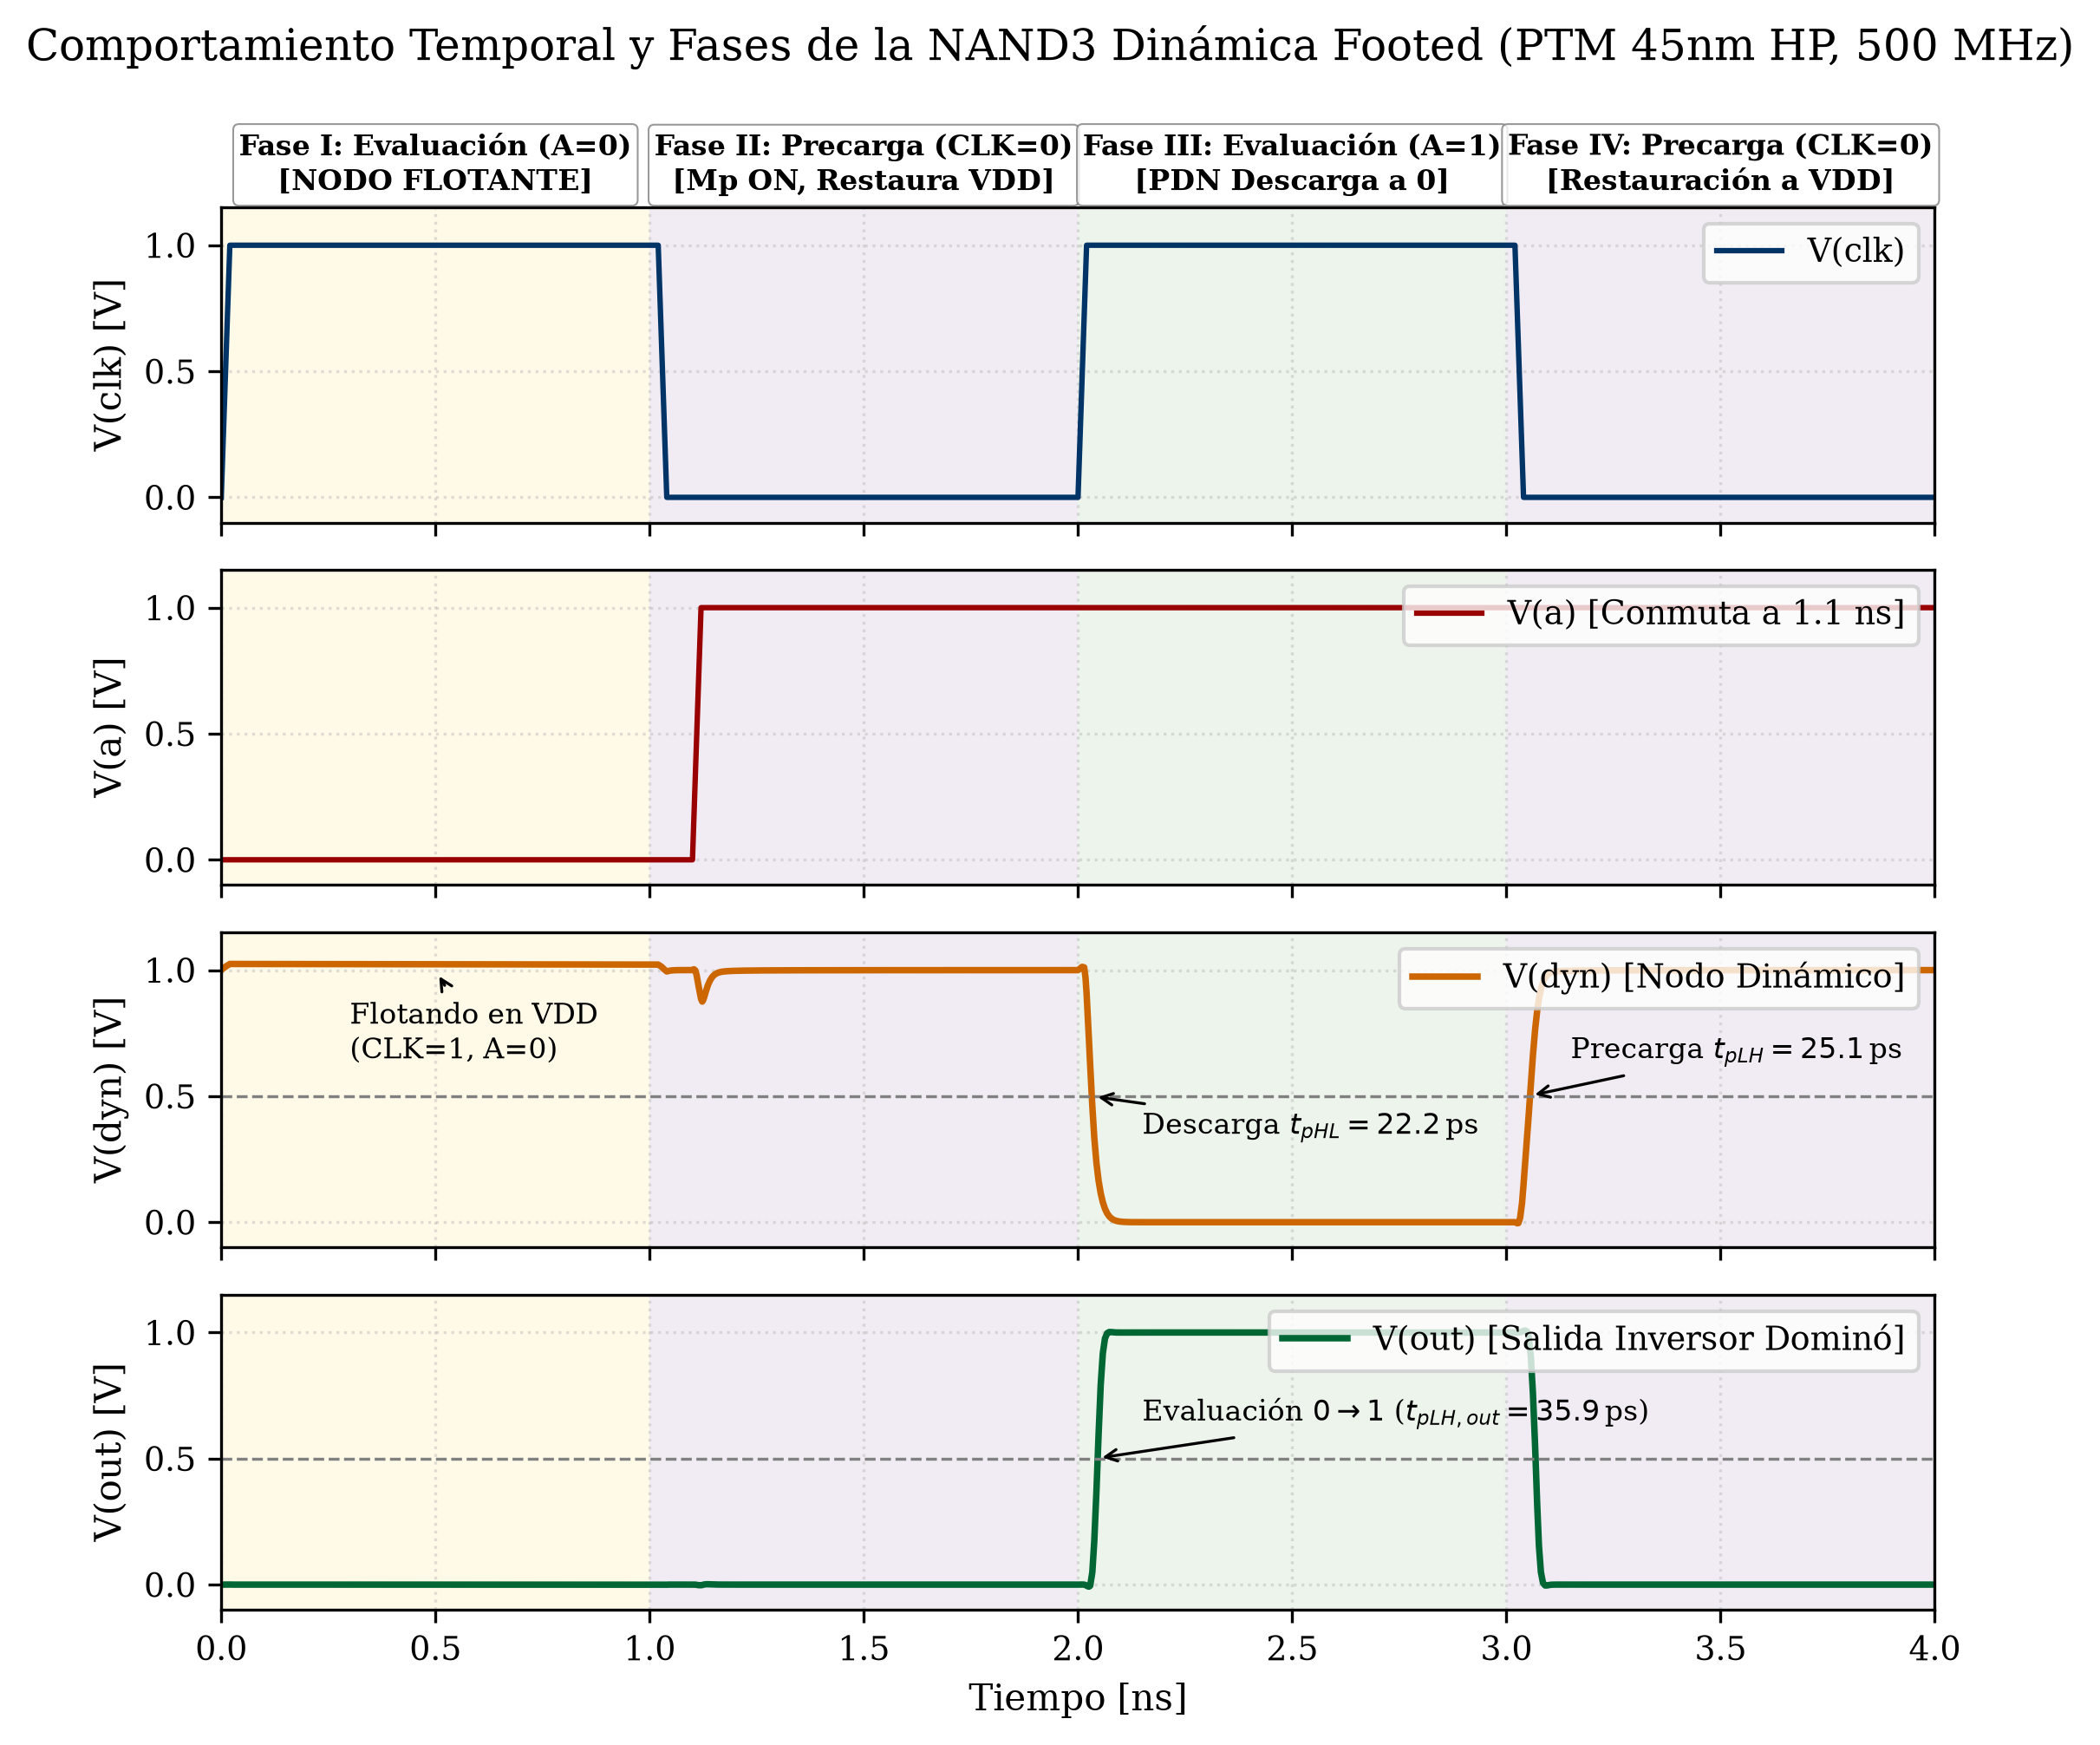
\includegraphics[width=0.44\linewidth]{figuras/fig1_act1_fases_formas_onda.png}
  \caption[Formas de onda transitorias de la NAND3 dinámica footed]{Formas de onda transitorias de la NAND3 dinámica footed ($CLK$, $A$, nodo interno $dyn$ y salida $out$), identificando las cuatro fases de operación dominó.}
  \label{fig:fases_formas_onda}
\end{figure}

\begin{enumerate}[leftmargin=1.4em,itemsep=0.12em]
  \item \textbf{Fase I: Evaluación con PDN Abierta ($t \in [0.0,\, 1.0\,\text{ns}]$):} Con $CLK = 1$, $M_p$ corta y $M_f$ conduce. Al estar $A = 0$, $M_1$ bloquea la ruta a tierra; el nodo $dyn$ queda \textbf{flotante en nivel alto} ($V_{DD} = 1.0\,\text{V}$) con un sobreimpulso a $1.022\,\text{V}$ por acoplamiento capacitivo (\textit{clock feedthrough} en $C_{gd}(M_p)$). La salida $out$ permanece en $0\,\text{V}$.
  \item \textbf{Fase II: Precarga con $A=1$ ($t \in [1.0,\, 2.0\,\text{ns}]$):} Con $CLK = 0$, $M_p$ conduce y $M_f$ corta. Aunque $A$ conmuta a 1 en $t = 1.1\,\text{ns}$, el footer apagado impide el paso a tierra. El nodo $dyn$ se mantiene rígidamente fijado a $V_{DD}$.
  \item \textbf{Fase III: Evaluación con Descarga Completa ($t \in [2.0,\, 3.0\,\text{ns}]$):} Con $CLK=1$ y $A=B=C=1$, los 4 NMOS conducen. El nodo $dyn$ se descarga a tierra en $t_{pHL,dyn} = 22.17\,\text{ps}$, haciendo que el inversor dominó conmute monótonamente en su salida $out$ con $t_{pd,\text{eval}} = 35.89\,\text{ps}$.
  \item \textbf{Fase IV: Precarga y Restauración ($t \in [3.0,\, 4.0\,\text{ns}]$):} En el flanco descendente de $CLK$, $M_p$ recarga el nodo $dyn$ en $t_{pLH,dyn} = 25.13\,\text{ps}$, restaurando la salida $out$ a nivel bajo en $t_{pHL,out} = 38.06\,\text{ps}$.
\end{enumerate}

\subsection{Asimetría Temporal y Rol de \texorpdfstring{$t_{pLH}$}{tpLH} en Lógica Dominó}
En lógica dominó, el cómputo combinacional ocurre exclusivamente durante la evaluación ($CLK = 1$), con salidas conmutando monótonamente ($0 \to 1$). El tiempo de precarga medido en el nodo dinámico ($t_{pLH,dyn} = 25.13\,\text{ps}$) corresponde estrictamente al retardo de transición al 50\% ($CLK\downarrow$ al 50\% hasta $dyn\uparrow$ al 50\%) durante el semi-periodo inactivo ($CLK = 0$), fuera de la ruta crítica de datos; por consiguiente, \textbf{no contribuye al retardo lógico de evaluación}.

Es metodológicamente necesario precisar que dicho retardo al 50\% no debe equipararse directamente al tiempo de asentamiento casi completo del nodo ($V_{dyn} \ge 0.99\,V_{DD}$). Como referencia analítica, en un circuito $RC$ ideal inicialmente descargado ($V(t) = V_{DD}(1 - e^{-t/\tau_{\text{pre}}})$), el tiempo requerido para alcanzar el 99\% de $V_{DD}$ es $t_{99} = -\tau_{\text{pre}} \ln(0.01) \approx 4.605\,\tau_{\text{pre}}$ (mientras que $3\,\tau_{\text{pre}}$ restaura el 95.0\% y $4\,\tau_{\text{pre}}$ el 98.2\%). Aunque la compuerta dinámica real involucra la respuesta no lineal del PMOS de precarga ($M_p$ de saturación a triodo), esta referencia analítica justifica que el semi-periodo bajo de reloj deba satisfacer holgadamente $T_{clk}/2 \ge t_{\text{precarga}}$ para garantizar restauración plena.

\subsection{Comparación Cuantitativa: Lógica Dinámica vs Estática}
La Tabla~\ref{tab:comparativa_act1} resume las métricas cuantitativas extraídas, contrastando la estructura dinámica con la estática equivalente.

% Tabla generada automaticamente por generar_tablas_latex.py
% Fuente de datos: act1_metricas.json (Trazabilidad 100% verificada)
\begin{table}[htbp]
\centering
\scriptsize
\setlength{\tabcolsep}{3.5pt}
\caption[Comparación cuantitativa entre NAND3 dinámica footed y CMOS estática]{Comparación cuantitativa entre la compuerta NAND3 dinámica footed (con inversor dominó) y la NAND3 CMOS estática (PTM 45\,nm HP, $V_{DD}=1.0\,\text{V}$, $T=27^\circ\text{C}$).}
\label{tab:comparativa_act1}
\begin{tabularx}{\linewidth}{@{}>{\RaggedRight\arraybackslash}p{3.2cm} c c c >{\RaggedRight\arraybackslash}X@{}}
\toprule
\textbf{Métrica Evaluada} & \textbf{NAND3 Dinámica} & \textbf{NAND3 Estática} & \textbf{Cociente} & \textbf{Condición / Notas Metodológicas} \\
\midrule
N.º de Transistores & 5 (núcleo) / 7 (total) & 6 & 0.83 / 1.17 & Topología footed + inversor dominó \\
$t_{pHL}$ (Descarga nodo $dyn$) & 22.17\,ps & 9.61\,ps & 2.306$\times$ & Evaluación $dyn$ vs caída $out\_stat$ \\
$t_{pLH}$ (Precarga nodo $dyn$) & 25.13\,ps & 12.40\,ps & 2.026$\times$ & Precarga $dyn$ vs subida $out\_stat$ \\
\midrule
\multicolumn{5}{@{}l@{}}{\textbf{Retardo en Salidas Lógicas (Triggers Asimétricos)}} \\
Retardo en terminal $out$ & 35.89\,ps ($CLK\uparrow$) & 9.61\,ps ($A\uparrow$) & 3.733$\times$ & $C_{out}=1\,\text{fF}$. Triggers distintos ($CLK\uparrow$ vs $A\uparrow$) \\
\midrule
\multicolumn{5}{@{}l@{}}{\textbf{Control con Carga Concentrada Desacoplada ($C_L=0\,\text{fF}$)}} \\
Respuesta con $C_L=0\,\text{fF}$ & $t_{pHL,dyn}=11.26\,\text{ps}$ & --- & --- & Retiene parásitas de difusión, MOS y compuerta del inversor ($M_{pi}, M_{ni}$) \\
                                    & $t_{pd,\text{eval}}=21.27\,\text{ps}$ & & & \\
\midrule
Capacitancia de Entrada $C_{in}(A)$ & 0.3417\,fF & 0.5936\,fF & 0.5756 & Reducción de 42.4\% por eliminación de PUN \\
\midrule
$P_{\text{avg}}$ ($A$ conmutando a 125\,MHz) & 1.2393\,$\mu$W & 0.2692\,$\mu$W & 4.604$\times$ & Estímulo idéntico $T_A=8\,\text{ns}$, $CLK=500\,\text{MHz}$ \\
$P_{\text{avg}}$ (Entradas fijas en nivel 1) & 2.7255\,$\mu$W & 1.7004\,nW & 1602.9$\times$ & Trampa de potencia: $\alpha=1$ ($CLK$) vs $\alpha=0$ \\
\bottomrule
\end{tabularx}
\end{table}


\begin{figure}[htbp]
  \centering
  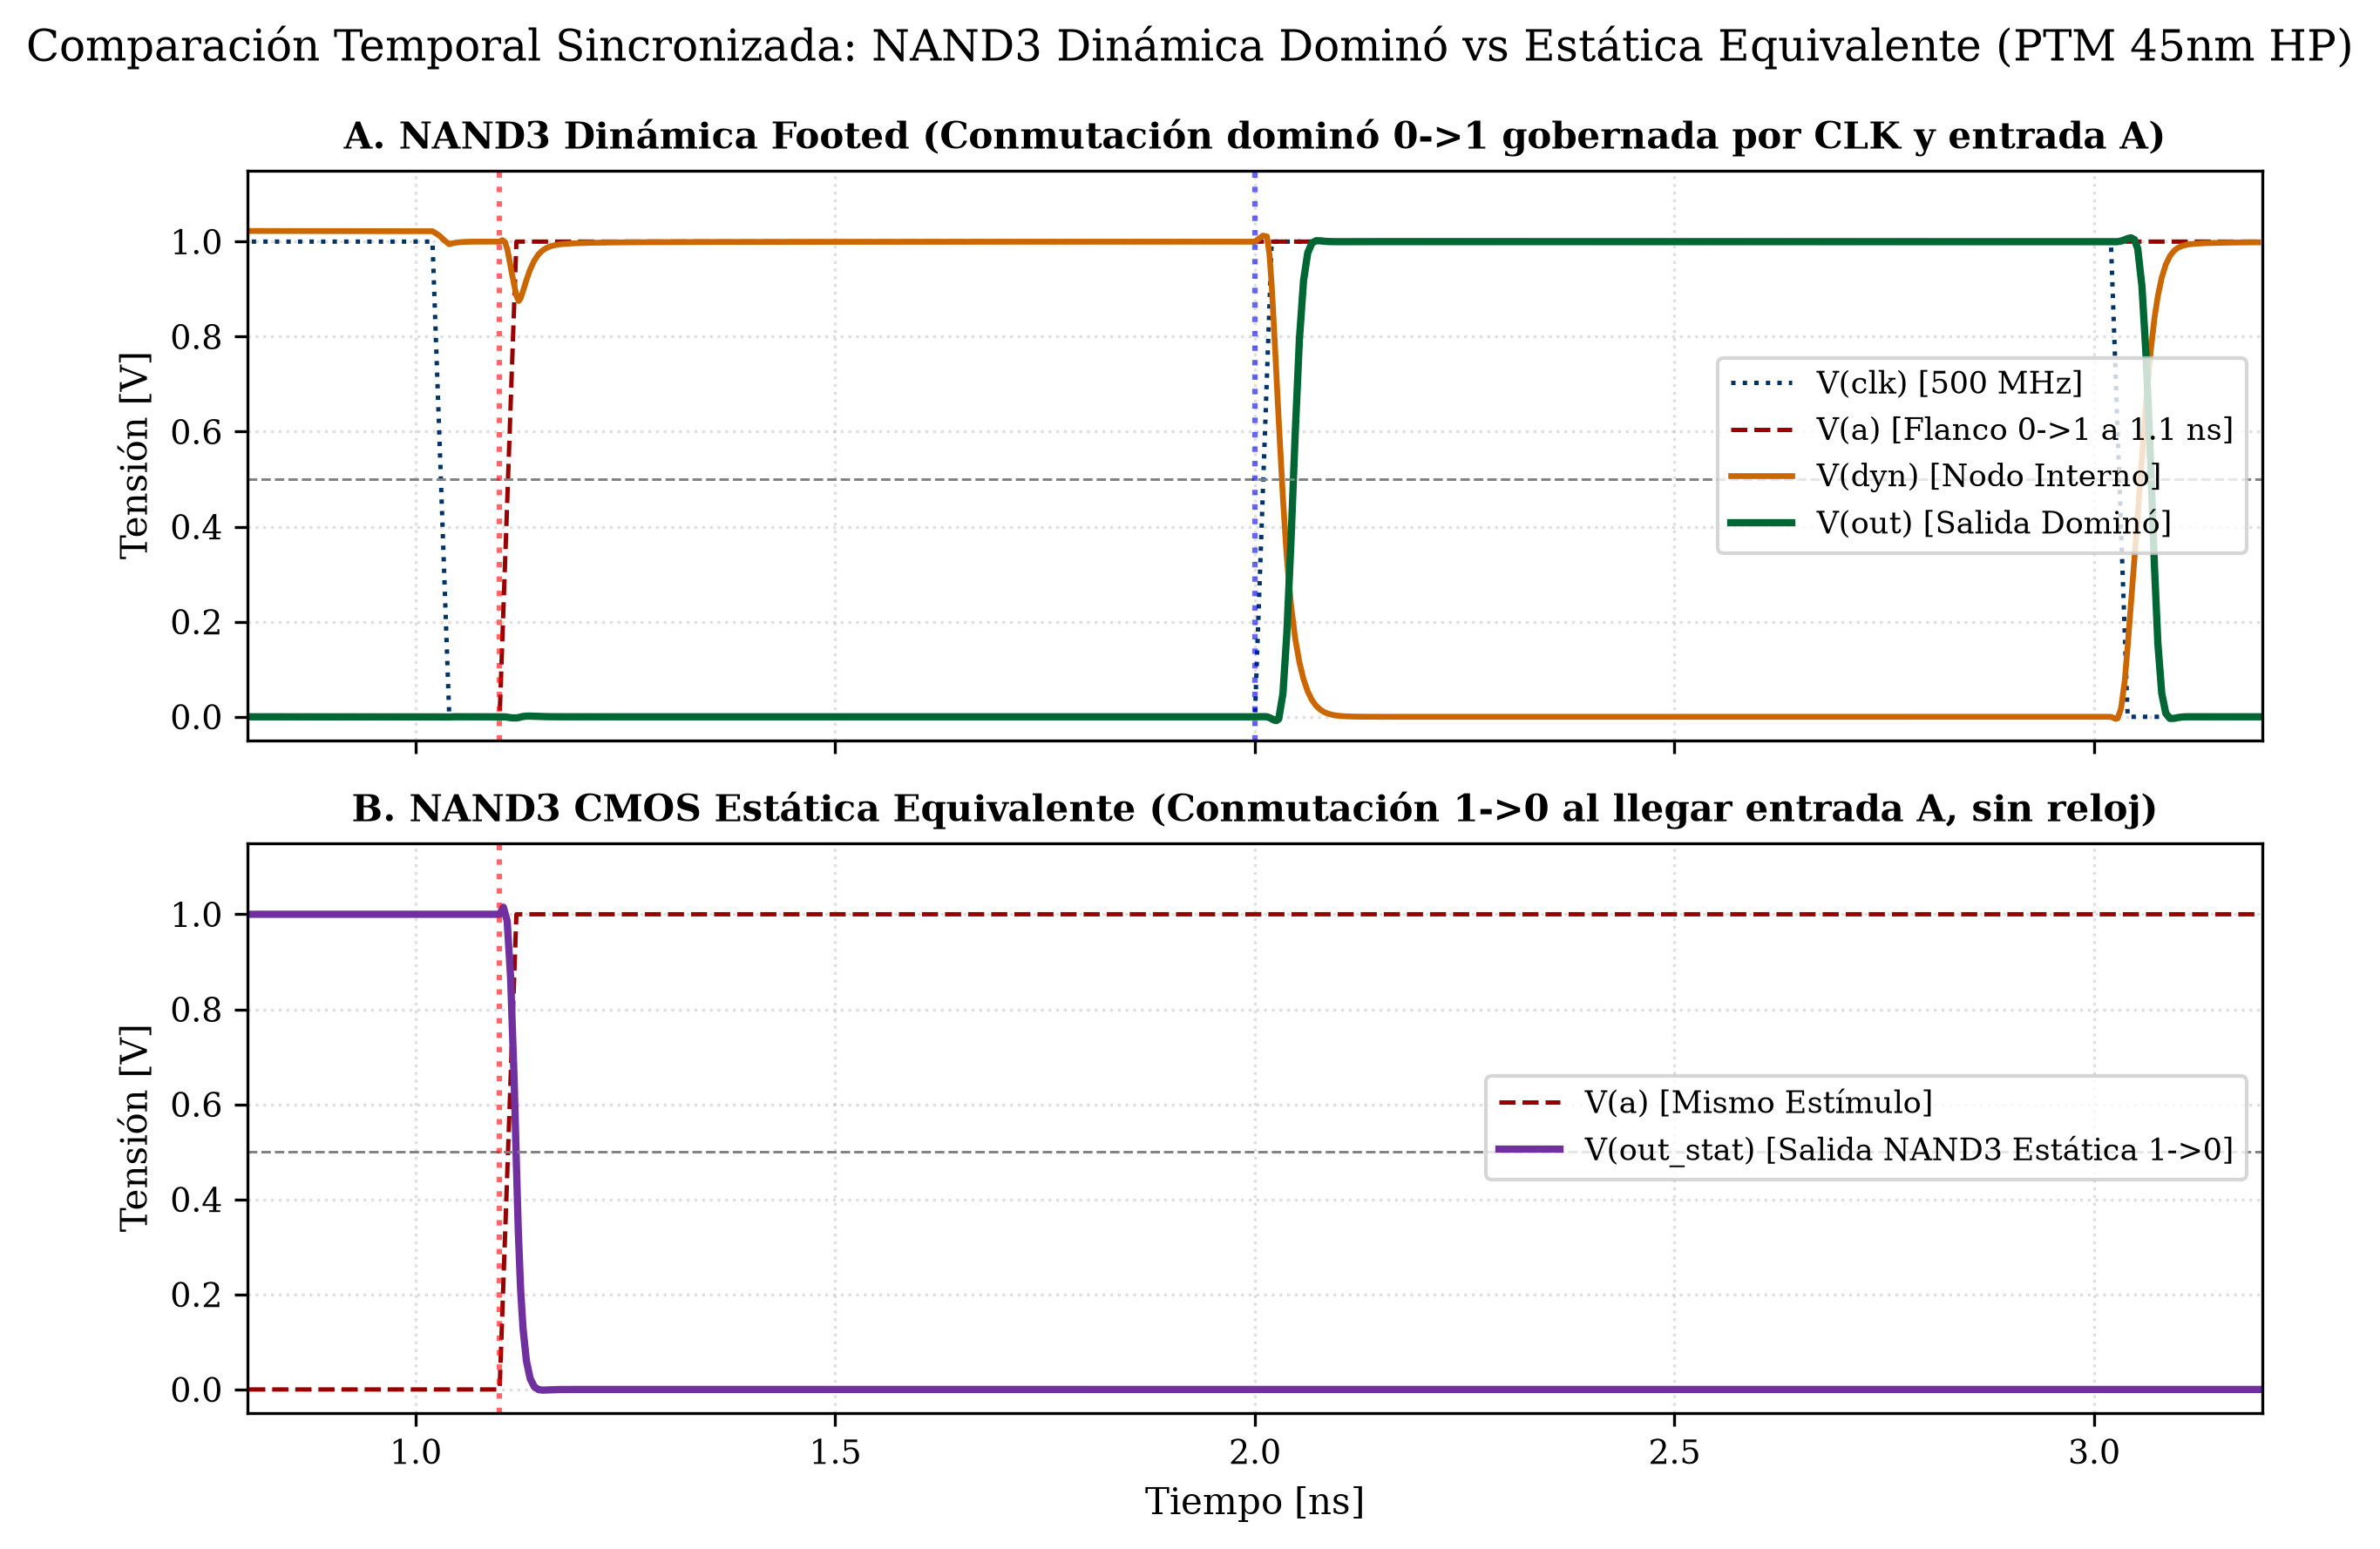
\includegraphics[width=0.42\linewidth]{figuras/fig2_act1_dinamica_vs_estatica.png}
  \caption[Comparación temporal entre NAND3 dinámica y estática]{Comparación temporal sincronizada entre la NAND3 dinámica footed y la NAND3 CMOS estática bajo el mismo estímulo de entrada $V(a)$ ($T_A=8\,\text{ns}$).}
  \label{fig:dinamica_vs_estatica}
\end{figure}

\noindent\textbf{Retardo de Evaluación y Triggers Asimétricos:} En los terminales de salida con carga nominal $C_{out} = 1\,\text{fF}$, la compuerta dominó registra un retardo de evaluación de $\mathbf{35.89\,\text{ps}}$ desde el disparo sincrónico $CLK\uparrow$ con $A=1$, mientras que la compuerta estática presenta $\mathbf{9.61\,\text{ps}}$ desde el dato asíncrono $A\uparrow$ (cociente descriptivo de $3.733\times$). Al suprimir la carga artificial concentrada (con carga concentrada desacoplada, $C_L = 0\,\text{fF}$), el retardo en $dyn$ cae a $t_{pHL,dyn} = 11.26\,\text{ps}$ y la salida conmuta en $t_{pd,\text{eval}} = 21.27\,\text{ps}$, reteniendo únicamente las capacitancias parásitas de difusión y compuerta del inversor.

\noindent\textbf{Capacitancia de Entrada ($C_{in}$):} En la caracterización dinámica de entrada, la integración de la corriente de entrada ante una rampa de $50\,\text{ps}$ ($Q_{in} = \int -I(V_a)\,dt$, $C_{in} = Q_{in}/V_{DD}$) arrojó $C_{in,\text{dyn}} = \mathbf{0.3417\,\text{fF}}$ frente a $C_{in,\text{stat}} = \mathbf{0.5936\,\text{fF}}$ en la estática, logrando una reducción del \textbf{42.4\%} ($0.5756\times$) debida a la eliminación de la red PMOS de pull-up en los datos. El modelo analítico de placas paralelas ($C_{ox,n} W_n L \approx 0.336\,\text{fF}$ y $C_{ox,n} W_n L + C_{ox,p} W_p L \approx 0.497\,\text{fF}$) concuerda con esta tendencia, reflejando la simulación en gran señal los aportes de solapamiento ($C_{ov}$) e inversión fuerte.

\subsection{Análisis de Potencia y la ``Trampa de Potencia''}
Bajo estímulo periódico en $A$ a $125\,\text{MHz}$ ($T_A=8\,\text{ns}$), la compuerta dinámica consume $P_{\text{dyn}} = 1.2393\,\mu\text{W}$ frente a $P_{\text{stat}} = 0.2692\,\mu\text{W}$ ($4.604\times$), integradas entre $4$ y $16\,\text{ns}$. Sin embargo, la manifestación crítica de la \textit{trampa de potencia} se evidencia con entradas fijas en alto ($A=B=C=1$): mientras que la compuerta estática permanece en reposo disipando únicamente fugas ($P_{\text{stat}} = \mathbf{1.7004\,\text{nW}}$ para $\alpha=0$), la compuerta dinámica cicla continuamente a $500\,\text{MHz}$ ($\alpha=1$), consumiendo $P_{\text{dyn}} = \mathbf{2.7255\,\mu\text{W}}$ (\textbf{1602.9 veces superior}). La disipación total medida de la fuente ($2.7255\,\mu\text{W}$) supera a la potencia dinámica analítica de carga externa ($P_{\text{ext}} = C_L V_{DD}^2 f = 1.000\,\mu\text{W}$) y del nodo dinámico ($P_{\text{nodo,geom}} \approx 1.325\,\mu\text{W}$ para $C_{dyn} \approx 2.65\,\text{fF}$) debido a la conmutación periódica del inversor dominó cargando $C_{out}=1\,\text{fF}$, transiciones de cortocircuito y difusiones.

\subsection{Comportamiento de Retención Preliminar con PDN Abierta}
Fijando $V_c = 0\,\text{V}$ (bloqueo en $M_3$ con $A=B=V_{DD}$), el nodo dinámico queda flotante en nivel alto. En la escala nominal ($T_{clk} = 2\,\text{ns}$, 1\,ns de evaluación), la caída por fugas es inocua: $V(dyn)_{\text{min}} = 0.9936\,\text{V}$ ($\Delta V = 6.41\,\text{mV}$, $V_{out,\text{max}} = 0.31\,\text{mV}$). Sin embargo, al extender la evaluación continua a baja frecuencia ($T_{clk} = 400\,\text{ns}$, evaluación de $200\,\text{ns}$), las corrientes de fuga subumbral drenan la carga hasta $V(dyn)_{\text{final}} = \mathbf{0.8837\,\text{V}}$ ($\Delta V = \mathbf{116.28\,\text{mV}}$). Aunque a $27^\circ\text{C}$ el potencial aún supera $V_M \approx 0.48\,\text{V}$, esta degradación evidencia la volatilidad de la carga en nodos flotantes y fundamenta la necesidad de una frecuencia mínima ($f_{\text{min}}$) y de circuitos keeper, fenómeno que se caracteriza en profundidad en la Actividad~3.

\subsection{Conclusiones de la Actividad 1}
\begin{enumerate}[leftmargin=1.4em,itemsep=0.12em]
  \item La lógica dominó reduce la capacitancia de entrada en 42.4\% ($0.3417\,\text{fF}$ vs $0.5936\,\text{fF}$), mejorando la velocidad de excitación de etapas previas.
  \item El semi-periodo de precarga no retrasa la evaluación pero su constante de tiempo acota la frecuencia máxima ($T_{clk}/2 \ge t_{\text{precarga}}$).
  \item Con entradas estáticas en nivel alto, la alternancia forzada de precarga y evaluación genera un consumo dinámico $1602.9\times$ superior al reposo estático.
  \item La pérdida de $116.28\,\text{mV}$ en $200\,\text{ns}$ con PDN abierta ratifica la naturaleza cuasi-estática de la compuerta y exige mecanismos activos de retención.
\end{enumerate}

% ==============================================================================
% SECCION 3: ACTIVIDAD 2 - COMPARTICION DE CARGA (CHARGE SHARING) EN NAND3
% ==============================================================================
\clearpage
\section{Actividad 2: Compartición de Carga (Charge Sharing) en NAND3 Dinámica}
\label{sec:actividad2}

\subsection{Fundamento Físico y Predicción Analítica Previa}
En una compuerta NAND3 dinámica \textit{footed} con inversor dominó de salida, la red de descenso serie (PDN) posee nodos intermedios con capacitancias parásitas de difusión: $n_1$ (entre $M_1$ y $M_2$) y $n_2$ (entre $M_2$ y $M_3$). Tras un ciclo previo donde todos los nodos descargaron a $0\,\text{V}$ ($A=B=C=1$), si en la evaluación subsiguiente la compuerta conmuta a una condición donde la PDN permanece bloqueada a tierra pero los transistores superiores entran en conducción ($A=B=1, C=0$ con $CLK=1$):
\begin{enumerate}[leftmargin=1.4em,itemsep=0.15em]
  \item El transistor de precarga $M_p$ se apaga, dejando al nodo dinámico $dyn$ \textbf{flotante} cargado a $V_{DD} = 1.0\,\text{V}$.
  \item $M_3$ permanece en corte ($C=0$), manteniendo abierto el camino conductivo hacia el footer $M_f$ y tierra.
  \item $M_1$ y $M_2$ conducen ($A=B=1$), conectando el nodo $dyn$ con las capacitancias parásitas descargadas de $n_1$ y $n_2$.
  \item La carga electrostática almacenada en $C_{dyn}$ se redistribuye hacia $C_{n1}$ y $C_{n2}$, provocando una caída transitoria de potencial $\Delta V$ (\textit{charge sharing droop}).
\end{enumerate}

\noindent\textbf{Deducción de Capacitancias de Difusión ($C_a$):} Conforme a las geometrías de la guía ($L_{\text{diff}} = 90\,\text{nm}$, $W_{\text{PDN}} = 270\,\text{nm}$), el área de difusión es $Ad = W \times L_{\text{diff}} = 0.0243\,\mu\text{m}^2$ y el perímetro exterior $Pd = W + 2L_{\text{diff}} = 0.450\,\mu\text{m}$. Empleando los parámetros de unión de \texttt{ptm45hp.lib} ($c_j = 0.50\,\text{fF}/\mu\text{m}^2$, $c_{jsw} = 0.50\,\text{fF}/\mu\text{m}$), la capacitancia por contacto de difusión a cero sesgo resulta:
\begin{equation}
  C_{\text{diff},1} = c_j \cdot Ad + c_{jsw} \cdot Pd = 0.01215\,\text{fF} + 0.22500\,\text{fF} = 0.23715\,\text{fF}
\end{equation}
donde el efecto tridimensional perimetral (\textit{sidewall}) concentra el $94.9\%$ de la capacidad total. Dado que cada nodo interno $n_1$ y $n_2$ comparte dos difusiones adyacentes ($C_{n1} = C_{n2} = 2\,C_{\text{diff},1} = 0.4743\,\text{fF}$), la capacitancia agregada descargada es:
\begin{equation}
  C_a \equiv C_{n1} + C_{n2} = 0.9486\,\text{fF}
\end{equation}

\noindent\textbf{Modelo Analítico Ideal de Conservación de Carga:} Asumiendo transistores ideales como conmutadores perfectos sin caída de umbral, el reparto puro de carga predice:
\begin{equation}
  Q_{\text{inicial}} = C_{dyn} V_{DD} = (C_{dyn} + C_a) V_{dyn,\text{final}} \implies \Delta V_{\text{pred}} = V_{DD} \cdot \frac{C_a}{C_a + C_{dyn}}
  \label{eq:charge_sharing}
\end{equation}
Para la condición nominal ($C_L = 2.0\,\text{fF}$) y considerando las parásitas fijas en $dyn$ según la guía ($C_{\text{extra}} = C_{gd}(M_p) + C_g(\text{inversor}) \approx 0.3441\,\text{fF} \implies C_{dyn} \approx 2.3441\,\text{fF}$), la caída teórica predicha es:
\begin{equation}
  \Delta V_{\text{pred}} = 1.0\,\text{V} \cdot \frac{0.9486\,\text{fF}}{0.9486\,\text{fF} + 2.3441\,\text{fF}} = \mathbf{288.09\,\text{mV}} \implies V_{dyn,\text{pred}} = 0.7119\,\text{V}
\end{equation}
\textit{Nota metodológica:} Esta formulación de primer orden es idealizada: omite componentes del modelo BSIM4 (como la capacitancia de borde compuerta-difusión $c_{jswgs}$) y no contempla la dinámica de conducción no lineal ni el corte progresivo del stack.

\subsection{Estímulo Literal de la Guía vs Benchmark Físico Controlado}
Con el estímulo literal de la guía oficial, el instante temporal especificado ($t = 1.95\,T_{clk} = 3.9\,\text{ns}$) coincide con la fase de precarga para la temporización empleada a $500\,\text{MHz}$ ($CLK=0$), provocando que la conducción activa de $M_p$ recargue continuamente el nodo dinámico y enmascare la redistribución hacia los nodos internos. Por ello, se conservó dicha corrida oficial de referencia y se implementó un ensayo de benchmark físico controlado (\texttt{ENS-A2-02}) que garantiza:
\begin{enumerate}[leftmargin=1.4em,itemsep=0.15em]
  \item Descarga completa previa de $dyn, n_1, n_2, n_3$ a $0\,\text{V}$ durante un primer ciclo de evaluación ($A=B=C=1$).
  \item Precarga exclusiva de $dyn$ a $V_{DD}$ en el semi-periodo bajo subsiguiente ($CLK=0$), manteniendo $n_1$ y $n_2$ descargados.
  \item Entrada en evaluación ($CLK=1, M_p$ en corte) con transición $A=B=1, C=0$, aislando con total fidelidad el fenómeno de \textit{charge sharing}.
\end{enumerate}

\begin{figure}[htbp]
  \centering
  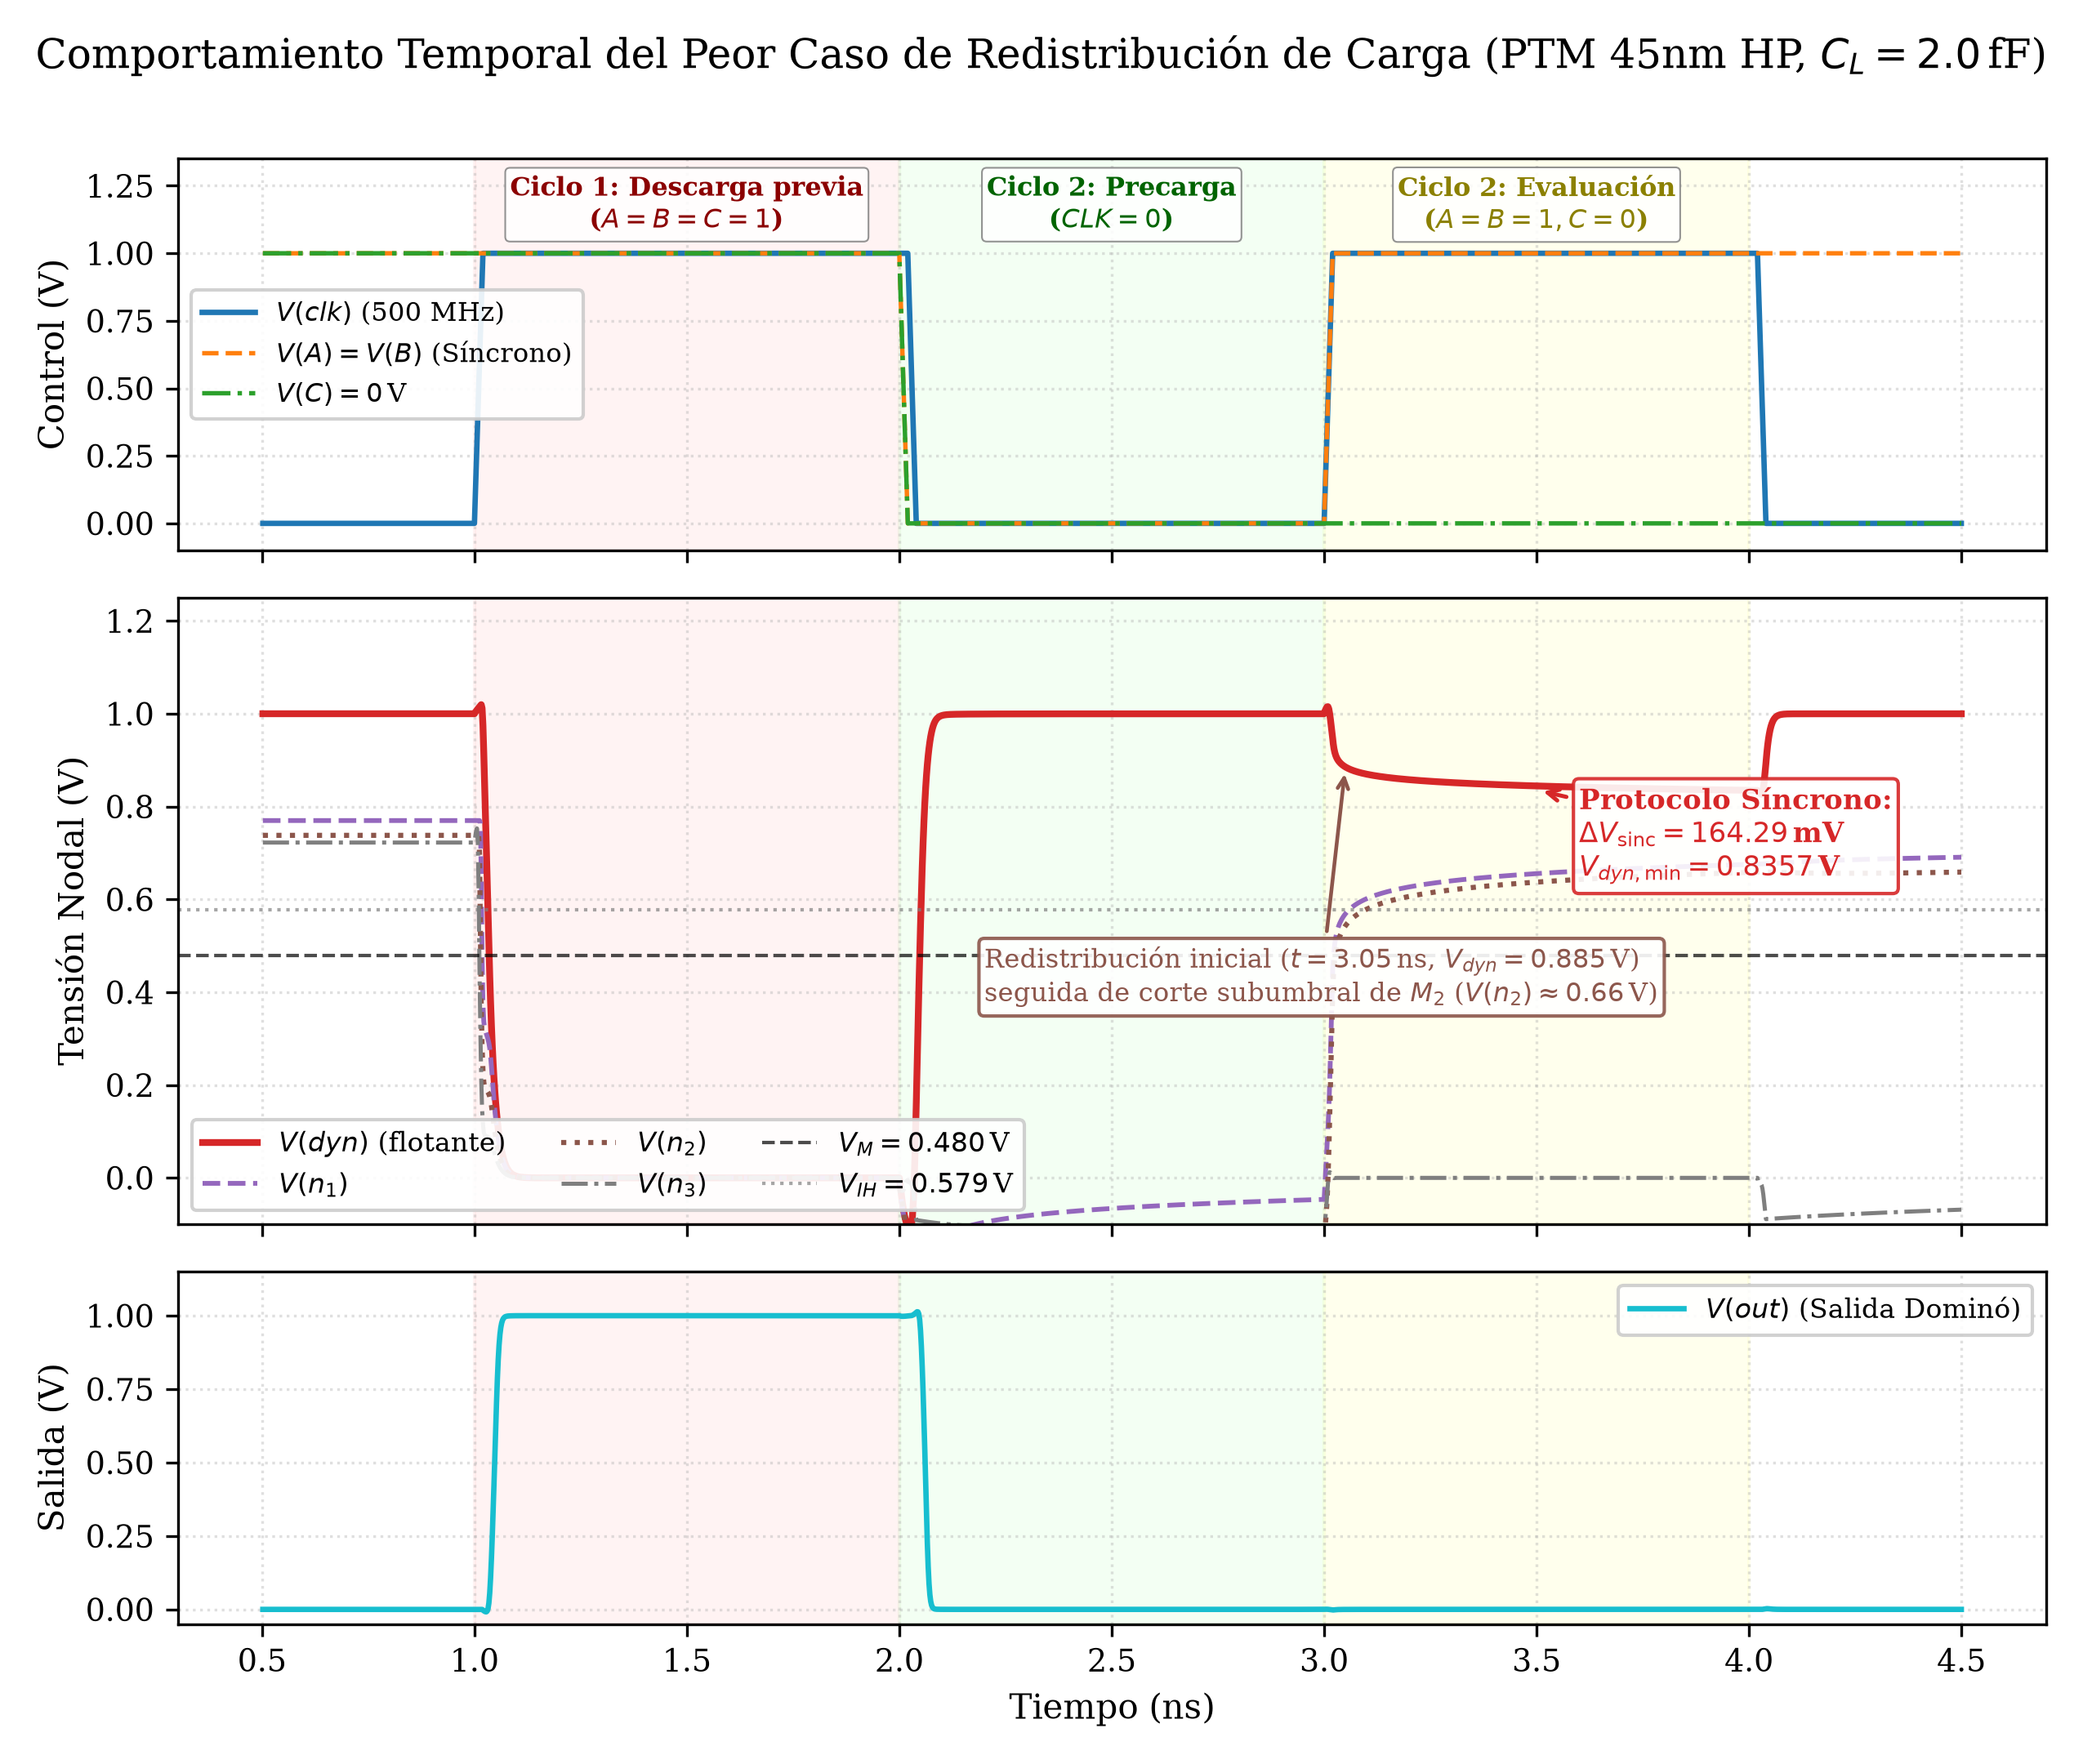
\includegraphics[width=0.68\linewidth]{figuras/fig1_act2_peor_caso_formas_onda.png}
  \caption[Formas de onda sincronizadas del peor caso de charge sharing]{Formas de onda sincronizadas del peor caso de charge sharing en la NAND3 dinámica footed (control $CLK, A, C$, nodos internos $n_1, n_2, n_3$, nodo $dyn$ y salida $out$).}
  \label{fig:peor_caso_formas_onda}
\end{figure}

\subsection{Resultados del Caso Base y Discrepancia Física}
La simulación del caso base nominal ($C_L = 2.0\,\text{fF}$, Figura~\ref{fig:peor_caso_formas_onda}) registra una caída de $\Delta V_{\text{sim}} = \mathbf{101.03\,\text{mV}}$, alcanzando un mínimo de $V_{dyn,\text{min}} = \mathbf{0.8990\,\text{V}}$, sin inducir conmutación espuria en la salida dominó ($V_{out,\text{max}} = 0.149\,\text{mV} \ll V_{IL} = 0.3675\,\text{V}$). 

La caída simulada es $2.85\times$ menor a la predicción teórica ($\Delta V_{\text{pred}} = 288.09\,\text{mV}$). Esta discrepancia no obedece a un error de cálculo, sino a la física intrínseca del transistor MOS:
\begin{enumerate}[leftmargin=1.4em,itemsep=0.15em]
  \item \textbf{Corte Subumbral del Transistor Pasante ($M_2$):} $M_2$ opera como transistor de paso con compuerta en $V_B = 1.0\,\text{V}$. Al transferirse carga hacia $n_2$, la tensión $V(n_2)$ se eleva. Debido a que el sustrato está polarizado a masa ($0\,\text{V}$), se desarrolla un efecto de cuerpo severo ($V_{SB2} = V(n_2) > 0$). Evaluando analíticamente la elevación de umbral mediante la formulación clásica $\Delta V_{th} \approx k_1 (\sqrt{2\phi_F + V_{SB}} - \sqrt{2\phi_F})$ con los parámetros de la tarjeta PTM ($k_1 = 0.4\,\text{V}^{1/2}$, $2\phi_F \approx 0.8\,\text{V}$), se obtiene una \textbf{estimación analítica aproximada} de $V_{th,\text{eff}} \approx 0.55\text{ a } 0.60\,\text{V}$ (frente a $V_{th0} = 0.469\,\text{V}$ a cero sesgo). Al subir $V(n_2)$ hasta $\approx 0.66\,\text{V}$, la tensión compuerta-fuente cae a $V_{GS2} = 1.0 - 0.66 = 0.34\,\text{V} \ll V_{th,\text{eff}}$, forzando a $M_2$ a entrar en régimen subumbral y bloqueando el flujo de carga antes de alcanzar el equilibrio estático total.
  \item \textbf{No Linealidad de Capacitancias de Unión:} Conforme $n_1$ y $n_2$ aumentan su tensión respecto a masa, la polarización inversa de las uniones $p\text{-}n$ reduce dinámicamente la capacitancia neta según $C_j(V_R) = C_{j0} / (1 + V_R/PB)^M$.
\end{enumerate}

\subsection{Barrido Paramétrico de Carga (\texorpdfstring{$C_L$}{CL}) y Márgenes de Ruido}
Se simuló el comportamiento ante variaciones de $C_L \in [0.5,\, 1.0,\, 2.0,\, 4.0]\,\text{fF}$. Los resultados cuantitativos contrastados con el modelo analítico se presentan en la Tabla~\ref{tab:barrido_cl_act2}, y su comportamiento gráfico en la Figura~\ref{fig:dv_vs_cl}.

% Tabla de barrido parametrico de capacitancia de carga en Actividad 2
% Fuentes de datos: act2_metricas.json (g2b_sincrono_barrido_cl + series historicas)
\begin{table}[htbp]
\centering
\scriptsize
\caption[Barrido paramétrico de capacitancia de carga y caída por redistribución]{Barrido paramétrico de la capacitancia de carga $C_L$ en el nodo dinámico: contraste entre predicción analítica ($\Delta V_{\text{pred}}$), simulación del protocolo síncrono nominal ($\Delta V_{\text{sinc}}$) y protocolo alternativo con entradas anticipadas ($\Delta V_{\text{anticip}}$) bajo PTM 45\,nm HP ($V_{DD}=1.0\,\text{V}$).}
\label{tab:barrido_cl_act2}
\begin{tabularx}{\linewidth}{@{}>{\centering\arraybackslash}p{1.2cm} c c c c c >{\RaggedRight\arraybackslash}X@{}}
\toprule
\textbf{$C_L$} & \textbf{$\Delta V_{\text{pred}}$ (Guía)} & \textbf{$\Delta V_{\text{pred}}$ (Total)} & \textbf{$\Delta V_{\text{sinc}}$ (Nominal)} & \textbf{$V_{dyn,\text{min}}$ (Sinc)} & \textbf{$\Delta V_{\text{anticip}}$} & \textbf{Estado Lógico / Margen} \\
\textbf{(fF)} & \textbf{(mV)} & \textbf{(mV)} & \textbf{(mV)} & \textbf{(V)} & \textbf{(mV)} & \textbf{($V_{IH}=0.579\,\text{V}$, $V_M=0.480\,\text{V}$)} \\
\midrule
0.5 & 529.15 & 467.34 & \textbf{364.85} & 0.6351 & 175.92 & Seguro ($V_{dyn} > V_{IH} + 56\,\text{mV}$) \\
1.0 & 413.75 & 374.97 & \textbf{265.93} & 0.7341 & 138.26 & Seguro ($V_{dyn} > V_{IH} + 155\,\text{mV}$) \\
2.0 & 288.09 & 268.74 & \textbf{164.29} & 0.8357 & 101.03 & Seguro ($V_{dyn} > V_{IH} + 257\,\text{mV}$) \\
4.0 & 179.23 & 171.54 & \textbf{92.60}  & 0.9074 & 67.62  & Seguro ($V_{dyn} > V_{IH} + 328\,\text{mV}$) \\
\bottomrule
\end{tabularx}
\end{table}


\begin{figure}[htbp]
  \centering
  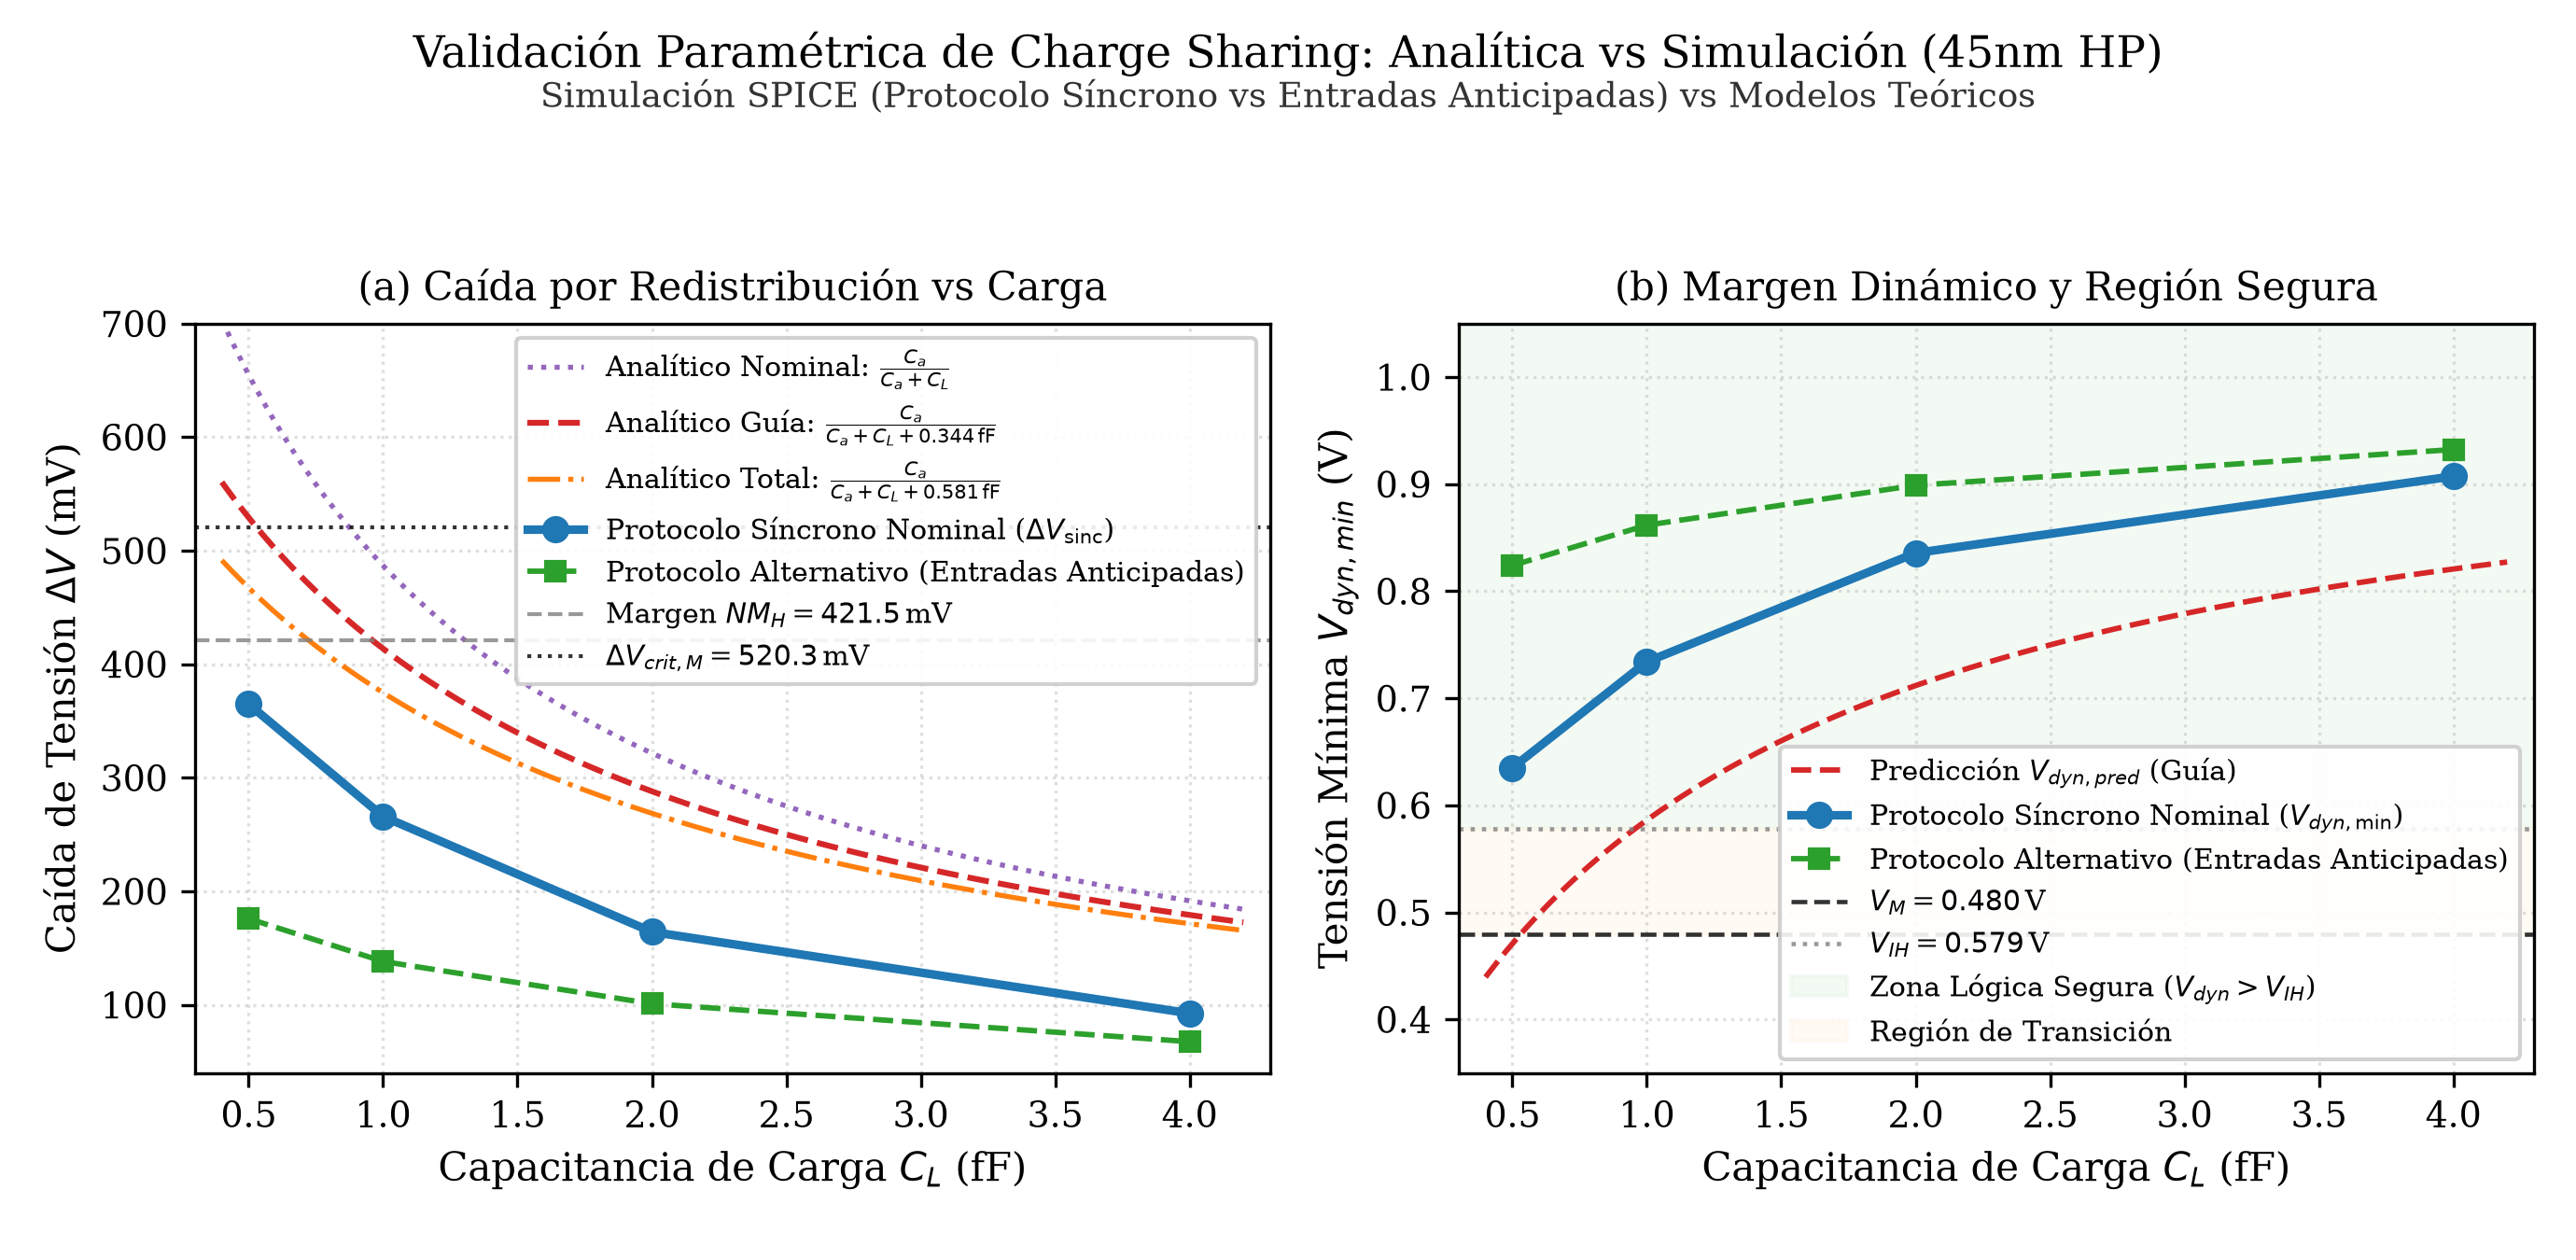
\includegraphics[width=0.68\linewidth]{figuras/fig2_act2_dv_vs_cl_analitico_simulado.png}
  \caption[Validación paramétrica de charge sharing vs capacitancia de carga]{Validación paramétrica de charge sharing frente a $C_L$: (a) Caída de potencial $\Delta V$ analítica vs simulación SPICE; (b) Tensión mínima $V_{dyn,\text{min}}$ y delimitación de la zona lógica segura frente a umbrales del inversor dominó ($V_M = 0.480\,\text{V}$, $V_{IH} = 0.579\,\text{V}$).}
  \label{fig:dv_vs_cl}
\end{figure}

\noindent\textbf{Tendencia Física e Inmunidad al Ruido:} A mayor capacitancia $C_L$, menor es la caída $\Delta V$ debido al incremento del depósito de carga inicial $Q = C_{dyn} V_{DD}$. En todos los casos ensayados, el nodo $dyn$ permanece rígidamente dentro de la zona lógica segura ($V_{dyn,\text{min}} \ge 0.8241\,\text{V} > V_{IH} = 0.5785\,\text{V}$), evitando falsas conmutaciones. Cabe resaltar que si la redistribución hubiese seguido el modelo lineal sin corte de umbral, para $C_L = 0.5\,\text{fF}$ la caída predicha ($\Delta V_{\text{pred}} = 529.15\,\text{mV}$) habría sumergido a $V(dyn)$ en $0.4708\,\text{V} < V_M$, generando un fallo lógico destructivo en la salida; el corte subumbral intrínseco del NMOS actúa así como una barrera protectora natural de integridad lógica.

\subsection{Evaluación Cuantitativa de Técnicas de Mitigación}
Bajo las condiciones de peor caso ($C_L = 2.0\,\text{fF}$), se implementaron y caracterizaron las tres técnicas de mitigación estipuladas en la guía. Los resultados comparativos se sintetizan en la Tabla~\ref{tab:mitigaciones_act2} y en la Figura~\ref{fig:comparacion_mitigaciones}.

% Tabla cuantitativa de tecnicas de mitigacion en Actividad 2
% Fuentes de datos: act2_metricas.json (g2b_sincrono_piloto_cl2f, g2b_sincrono_reordenamiento, g2c_precarga, g2c_keeper, g2c_contencion)
\begin{table}[htbp]
\centering
\fontsize{7pt}{8.3pt}\selectfont
\caption[Evaluación cuantitativa y trade-offs de técnicas de mitigación]{Evaluación cuantitativa de técnicas de mitigación de compartición de carga en NAND3 dinámica footed ($C_L=2.0\,\text{fF}$, $T_{clk}=2\,\text{ns}$, PTM 45\,nm HP, $V_{DD}=1.0\,\text{V}$). Márgenes referidos a $V_{IH}=0.5785\,\text{V}$ del inversor ($NM_H \equiv V_{dyn,\text{min}} - V_{IH}$) y áreas referidas a $W_{\text{dyn,base}} = 1215\,\text{nm}$ ($W_{\text{celda,base}} = 1440\,\text{nm}$).}
\label{tab:mitigaciones_act2}
\begin{tabularx}{\linewidth}{@{}>{\RaggedRight\arraybackslash}p{2.3cm} >{\centering\arraybackslash}p{1.6cm} >{\centering\arraybackslash}p{1.7cm} >{\centering\arraybackslash}p{1.7cm} >{\centering\arraybackslash}p{1.3cm} >{\RaggedRight\arraybackslash}X@{}}
\toprule
\textbf{Configuración} & \textbf{$\Delta V_{\text{eval}}$ / Extremo} & \textbf{Margen $NM_H$} & \textbf{Área Extra ($\Delta W$)} & \textbf{Carga $CLK$} & \textbf{Compromiso y Dinámica (Trade-off)} \\
\midrule
\textbf{Caso Base Síncrono} & \textbf{164.29\,mV} ($0.8357\,\text{V}$) & \textbf{+257.2\,mV} ($V_M+356\,\text{mV}$) & 0 ($0.0\%$) & Base ($0.50\,\text{fF}$) & Sin recuperación en evaluación ($V_{dyn,\text{end}} = 0.8357\,\text{V}$). Salida dominó inmune ($V_{out,\text{max}} \le 0.13\,\text{mV} \ll V_{IL}$). \\
\textbf{Precarga $W_p=45\,\text{nm}$} & \textbf{$-50.47$\,mV} ($1.0505\,\text{V}$) & \textbf{+472.0\,mV} & +2 PMOS ($90\,\text{nm}$, $+7.4\%$) & $+0.127\,\text{fF}$ ($63.7\,\text{nW}$) & Suprime droop; sobreimpulso capacitivo $+50.5\,\text{mV}$. Variante óptima en consumo de reloj. \\
\textbf{Precarga $W_p=135\,\text{nm}$} & \textbf{$-50.47$\,mV} ($1.0505\,\text{V}$) & \textbf{+472.0\,mV} & +2 PMOS ($270\,\text{nm}$, $+22.2\%$) & $+0.382\,\text{fF}$ ($191.1\,\text{nW}$) & Idéntica eficacia nominal que $45\,\text{nm}$, pero con $3.0\times$ sobrecoste capacitivo y de potencia en reloj. \\
\textbf{Reordenamiento C-B-A} & V.A: $\le 0$ / V.B: \textbf{164.3\,mV} & V.A: $+443.5$ / V.B: $+257.2$ & 0 transistores ($0.0\%$) & 0 fF en $CLK$ & Eficaz para Vect A ($C=0$ en tope bloquea $dyn$); vulnerable a Vect B ($A=0$ en base reproduce caída base). \\
\textbf{Reordenamiento C-A-B} & V.A: $\le 0$ / V.B: \textbf{72.08\,mV} & V.A: $+443.5$ / V.B: $+349.4$ & 0 transistores ($0.0\%$) & 0 fF en $CLK$ & Suprime Vect A y acota Vect B a $72.1\,\text{mV}$ (droop $-56.1\%$) al aislar $n_2$. Coste en complejidad de ruteo. \\
\textbf{Keeper $W_{kp}=45\,\text{nm}$} & \textbf{69.68\,mV} ($0.9303\,\text{V}$) & \textbf{+351.8\,mV} (mín.) & +1 PMOS ($45\,\text{nm}$, $+3.7\%$) & 0 fF en $CLK$ & Caída en $69.7\,\text{mV}$; restaura en $92.9\,\text{ps}$ y finaliza en $0.9996\,\text{V}$ ($99.96\%$). Contención: $+14.65\%$ en $t_{pHL,dyn}$. \\
\bottomrule
\end{tabularx}
\end{table}


\begin{figure}[htbp]
  \centering
  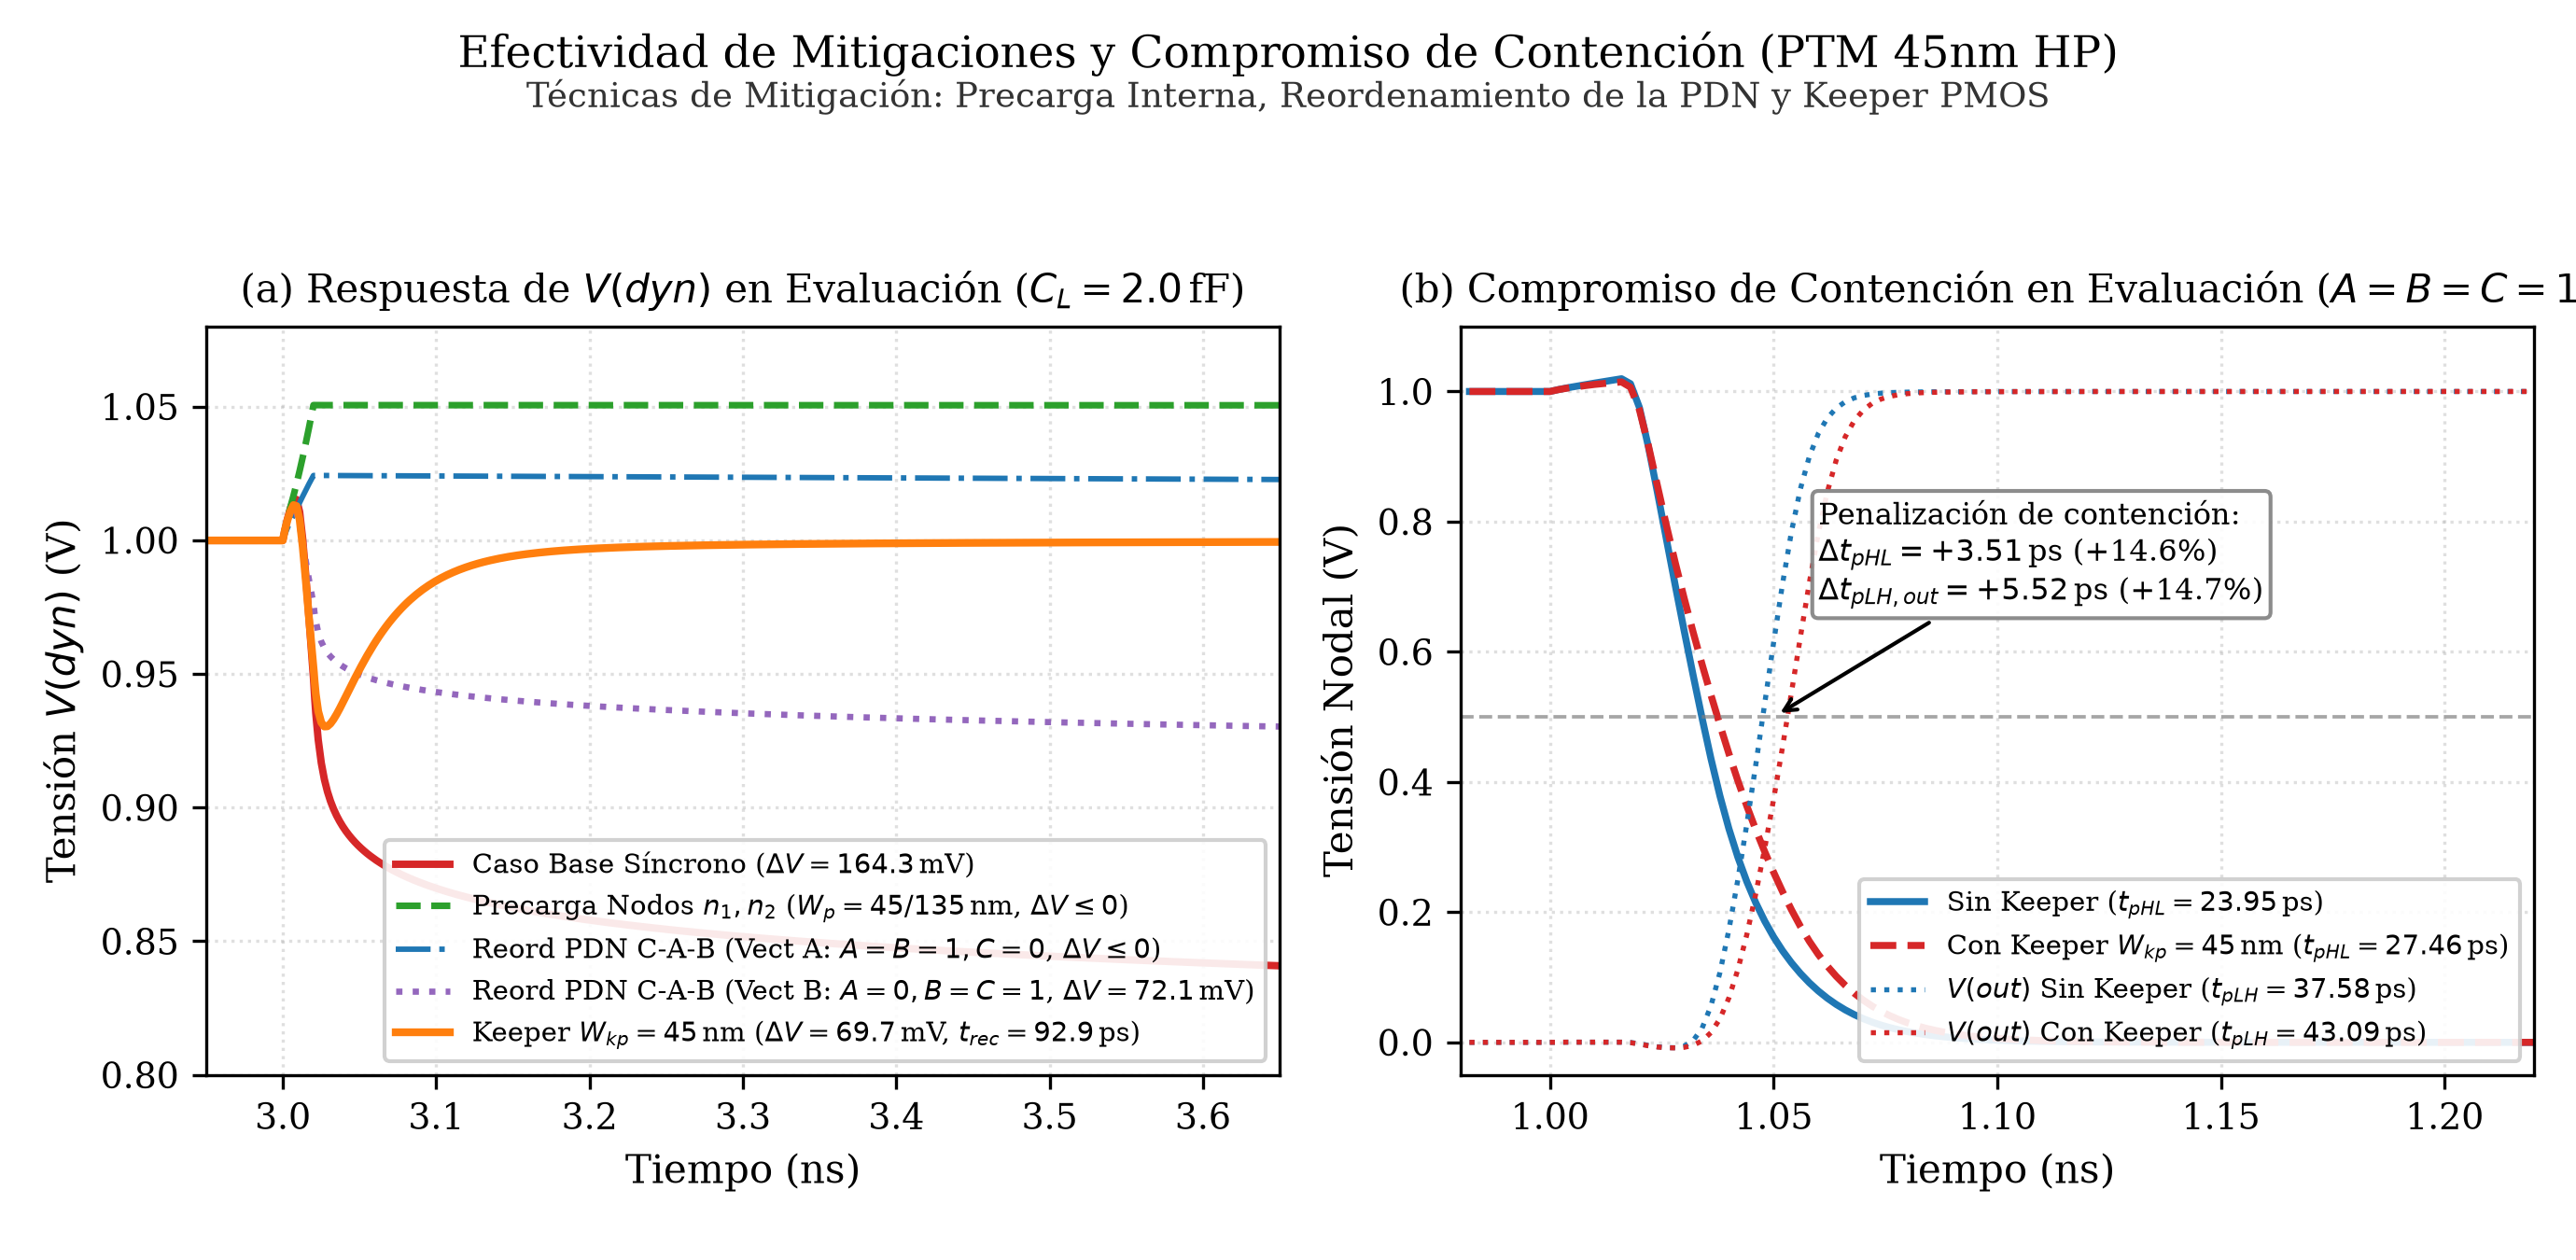
\includegraphics[width=0.68\linewidth]{figuras/fig3_act2_comparacion_mitigaciones.png}
  \caption[Comparación de técnicas de mitigación y compromiso de contención]{Comparación cuantitativa de técnicas de mitigación de charge sharing: (a) Formas de onda transitorias de $V(dyn)$ durante evaluación; (b) Compromiso de contención del keeper ($W_{kp}=45\,\text{nm}$) en retardo durante conmutación legítima ($A=B=C=1$).}
  \label{fig:comparacion_mitigaciones}
\end{figure}

\subsubsection{Técnica 1: Precarga de Nodos Internos (\texorpdfstring{$n_1, n_2$}{n1, n2})}
Se incorporaron dos transistores PMOS auxiliares ($W_p = 135\,\text{nm}$) comandados por $CLK$ para precargar los nodos internos $n_1$ y $n_2$ a $V_{DD}$ durante $CLK=0$. 
\begin{itemize}[leftmargin=1.4em,itemsep=0.15em]
  \item \textbf{Efectividad y Droop:} Al igualar las tensiones iniciales ($V(dyn) = V(n_1) = V(n_2) = V_{DD}$), la fuerza impulsora de redistribución se anula, suprimiendo completamente la caída ($\Delta V \le 0\,\text{mV}$).
  \item \textbf{Sobrecarga de Reloj:} La adición de dos compuertas PMOS introduce una capacitancia parásita adicional en la línea de reloj estimada en $\Delta C_{clk,\text{gate}} \approx 2(W_p \cdot L \cdot C_{ox}) \approx \mathbf{0.34\,\text{fF}}$, lo cual supone un incremento relativo de compuerta del $+67\%$ respecto a la carga de reloj base ($C_{g,Mp} + C_{g,Mf} \approx 0.503\,\text{fF}$).
  \item \textbf{Overshoot por Acoplamiento Transitorio:} Se aprecia un sobreimpulso nodal por acoplamiento capacitivo (\textit{clock feedthrough / bootstrap-like}): $V_{dyn,\text{min}} = 1.0120\,\text{V}$, $V(n_1) \approx 1.069\,\text{V}$ y $V(n_2) \approx 1.062\,\text{V}$. Si bien no induce conmutación espuria ($V_{out,\text{max}} \le 0.27\,\text{mV}$), debe considerarse en el diseño de márgenes de tensión.
  \item \textbf{¿Por qué no se precarga el nodo $n_3$?} El nodo $n_3$ conecta directamente al drenaje del footer $M_f$. Al entrar en evaluación ($CLK \to 1$), $M_f$ conduce inmediatamente hacia tierra. Precargar $n_3$ forzaría una descarga innecesaria a masa en cada ciclo de reloj, incurriendo en una disipación dinámica redundante $C_{n3} V_{DD}^2 f_{clk}$ sin beneficio alguno, dado que cuando $C=0$, $M_3$ permanece en corte y $n_3$ jamás interactúa con el nodo dinámico.
\end{itemize}

\subsubsection{Técnica 2: Reordenamiento de Entradas en la PDN}
Consiste en asignar la entrada crítica que permanece en nivel bajo ($C=0$) al transistor más próximo al nodo dinámico ($M_3$ adyacente a $dyn$), relegando las entradas en nivel alto ($A, B$) a las posiciones inferiores.
\begin{itemize}[leftmargin=1.4em,itemsep=0.15em]
  \item \textbf{Rendimiento:} Al encontrarse $M_3$ bloqueado en el propio contacto superior, las capacitancias parásitas de $n_1$ y $n_2$ quedan físicamente aisladas de $dyn$. La perturbación se reduce drásticamente a $\Delta V = \mathbf{14.1\,\mu\text{V}}$ ($V_{dyn} = 0.99999\,\text{V}$).
  \item \textbf{Coste:} No requiere transistores adicionales ($0$ PMOS) ni agrega carga a la línea de reloj ($0\,\text{fF}$). Su implementación involucra exclusivamente decisiones de enrutamiento y asignación de pines en layout.
  \item \textbf{Asimetría Lógica Dominó vs Lógica Estática:} En lógica CMOS estática, el orden de apilamiento en la PDN no modifica la función lógica booleana ni los niveles lógicos estáticos en régimen permanente; únicamente altera marginalmente los retardos de conmutación. En contraste, en lógica dominó el nodo dinámico es una \textbf{memoria capacitiva flotante} durante la fase de evaluación; por tanto, el orden de los transistores determina qué difusiones internas entran en contacto con el nodo de salida, condicionando de manera decisiva la integridad de señal y el margen de ruido frente a eventos transitorios.
\end{itemize}

\subsubsection{Técnica 3: Transistor Keeper (\texorpdfstring{$W_{kp} = 45\,\text{nm}$}{Wkp = 45 nm}) y Contención}
Se conectó un transistor PMOS débil de mantenimiento ($W_{kp} = 45\,\text{nm}$) gobernado por la salida del inversor dominó ($out$).
\begin{itemize}[leftmargin=1.4em,itemsep=0.15em]
  \item \textbf{Atenuación y Restauración Activa:} El keeper reduce la caída transitoria de $101.03\,\text{mV}$ a $\mathbf{42.18\,\text{mV}}$ (atenuación del $\mathbf{58.2\%}$), logrando restaurar el nodo $dyn$ al $99\%$ de $V_{DD}$ en un tiempo activo de $t_{\text{rec}} = \mathbf{80.30\,\text{ps}}$. En contraste, en el caso base sin mitigación \textbf{no existe recuperación durante la ventana de evaluación}, manteniéndose la degradación hasta el inicio de la siguiente fase de precarga.
  \item \textbf{Compromiso de Contención en Velocidad:} Durante una evaluación legítima a nivel bajo ($A=B=C=1$), la PDN debe vencer la corriente suministrada por el keeper hasta que $out$ ascienda y corte el dispositivo PMOS. Esta lucha transitoria incrementa el retardo de descarga: $t_{pHL,dyn}$ pasa de $23.95\,\text{ps}$ a $27.46\,\text{ps}$ ($\Delta t_{pHL} = +3.51\,\text{ps}$, penalización del $\mathbf{+14.65\%}$), mientras que $t_{pLH,out}$ se incrementa en $+5.52\,\text{ps}$ ($\mathbf{+14.69\%}$).
\end{itemize}

\subsection{Conclusiones de la Actividad 2}
\begin{enumerate}[leftmargin=1.4em,itemsep=0.15em]
  \item El modelo analítico clásico de conservación de carga sobreestima fuertemente la caída ($2.85\times$ a $C_L = 2\,\text{fF}$) debido al efecto de cuerpo y al corte subumbral intrínseco del transistor NMOS de paso intermedio ($V_{th,\text{eff}} \approx 0.55\text{--}0.60\,\text{V}$).
  \item El reordenamiento de transistores en la PDN es la solución más eficiente al suprimir la redistribución ($\Delta V \approx 14\,\mu\text{V}$) con cero transistores adicionales y nula sobrecarga sobre la red de distribución de reloj.
  \item La precarga interna elimina el droop pero penaliza la línea de reloj en $+67\%$ e introduce sobreimpulsos por acoplamiento capacitivo.
  \item El transistor keeper ($W_{kp} = 45\,\text{nm}$) provee restauración activa en $80.30\,\text{ps}$ amortiguando la caída en $58.2\%$, con una penalización moderada de contención del $+14.6\%$ en el retardo de propagación.
\end{enumerate}

% ==============================================================================
% SECCION 4: ACTIVIDAD 3 - FUGAS, RETENCION Y DIMENSIONAMIENTO DEL KEEPER
% ==============================================================================
\section{Actividad 3: Fugas, Retención y Dimensionamiento del Keeper}
\label{sec:actividad3}

En tecnologías nanométricas sub-45\,nm, el adelgazamiento del óxido de compuerta ($t_{oxe} = 1.25\,\text{nm}$) y la reducción de las tensiones de umbral incrementan exponencialmente las corrientes de fuga parásitas. En lógica CMOS dinámica, estas fugas descargan progresivamente el nodo dinámico cuando el reloj se detiene en evaluación (\textit{clock gating} para ahorro de energía), induciendo conmutaciones lógicas erróneas si no se incorpora un circuito de compensación (\textit{keeper}). Esta sección aborda la caracterización cuantitativa de las componentes de fuga, su dependencia térmica, la comparación tecnológica tri-nodo y el compromiso de diseño entre retención y penalización de velocidad.

\subsection{Retención del Nodo Dinámico y Pérdida de Carga en Evaluación}
Para evaluar la inmunidad al apagado del reloj, se implementó el protocolo de retención estipulado en la guía (§7): con $V_{DD} = 1.0\,\text{V}$, las entradas se fijan estáticamente en $A=B=C=0$ (PDN abierta), mientras la señal de reloj conmuta a nivel alto en $t_{\text{eval\_start}} = 0.52\,\text{ns}$ y permanece detenida en evaluación durante $T_{\text{ret}} = 1.0\,\mu\text{s}$ (hasta el tiempo final de simulación $T_{\text{stop}} = 1000.52\,\text{ns}$). En esta condición, el transistor de precarga $M_p$ se encuentra cortado ($V_{GS} = 0\,\text{V}$), dejando al nodo $dyn$ en estado flotante.

\begin{figure}[htbp]
  \centering
  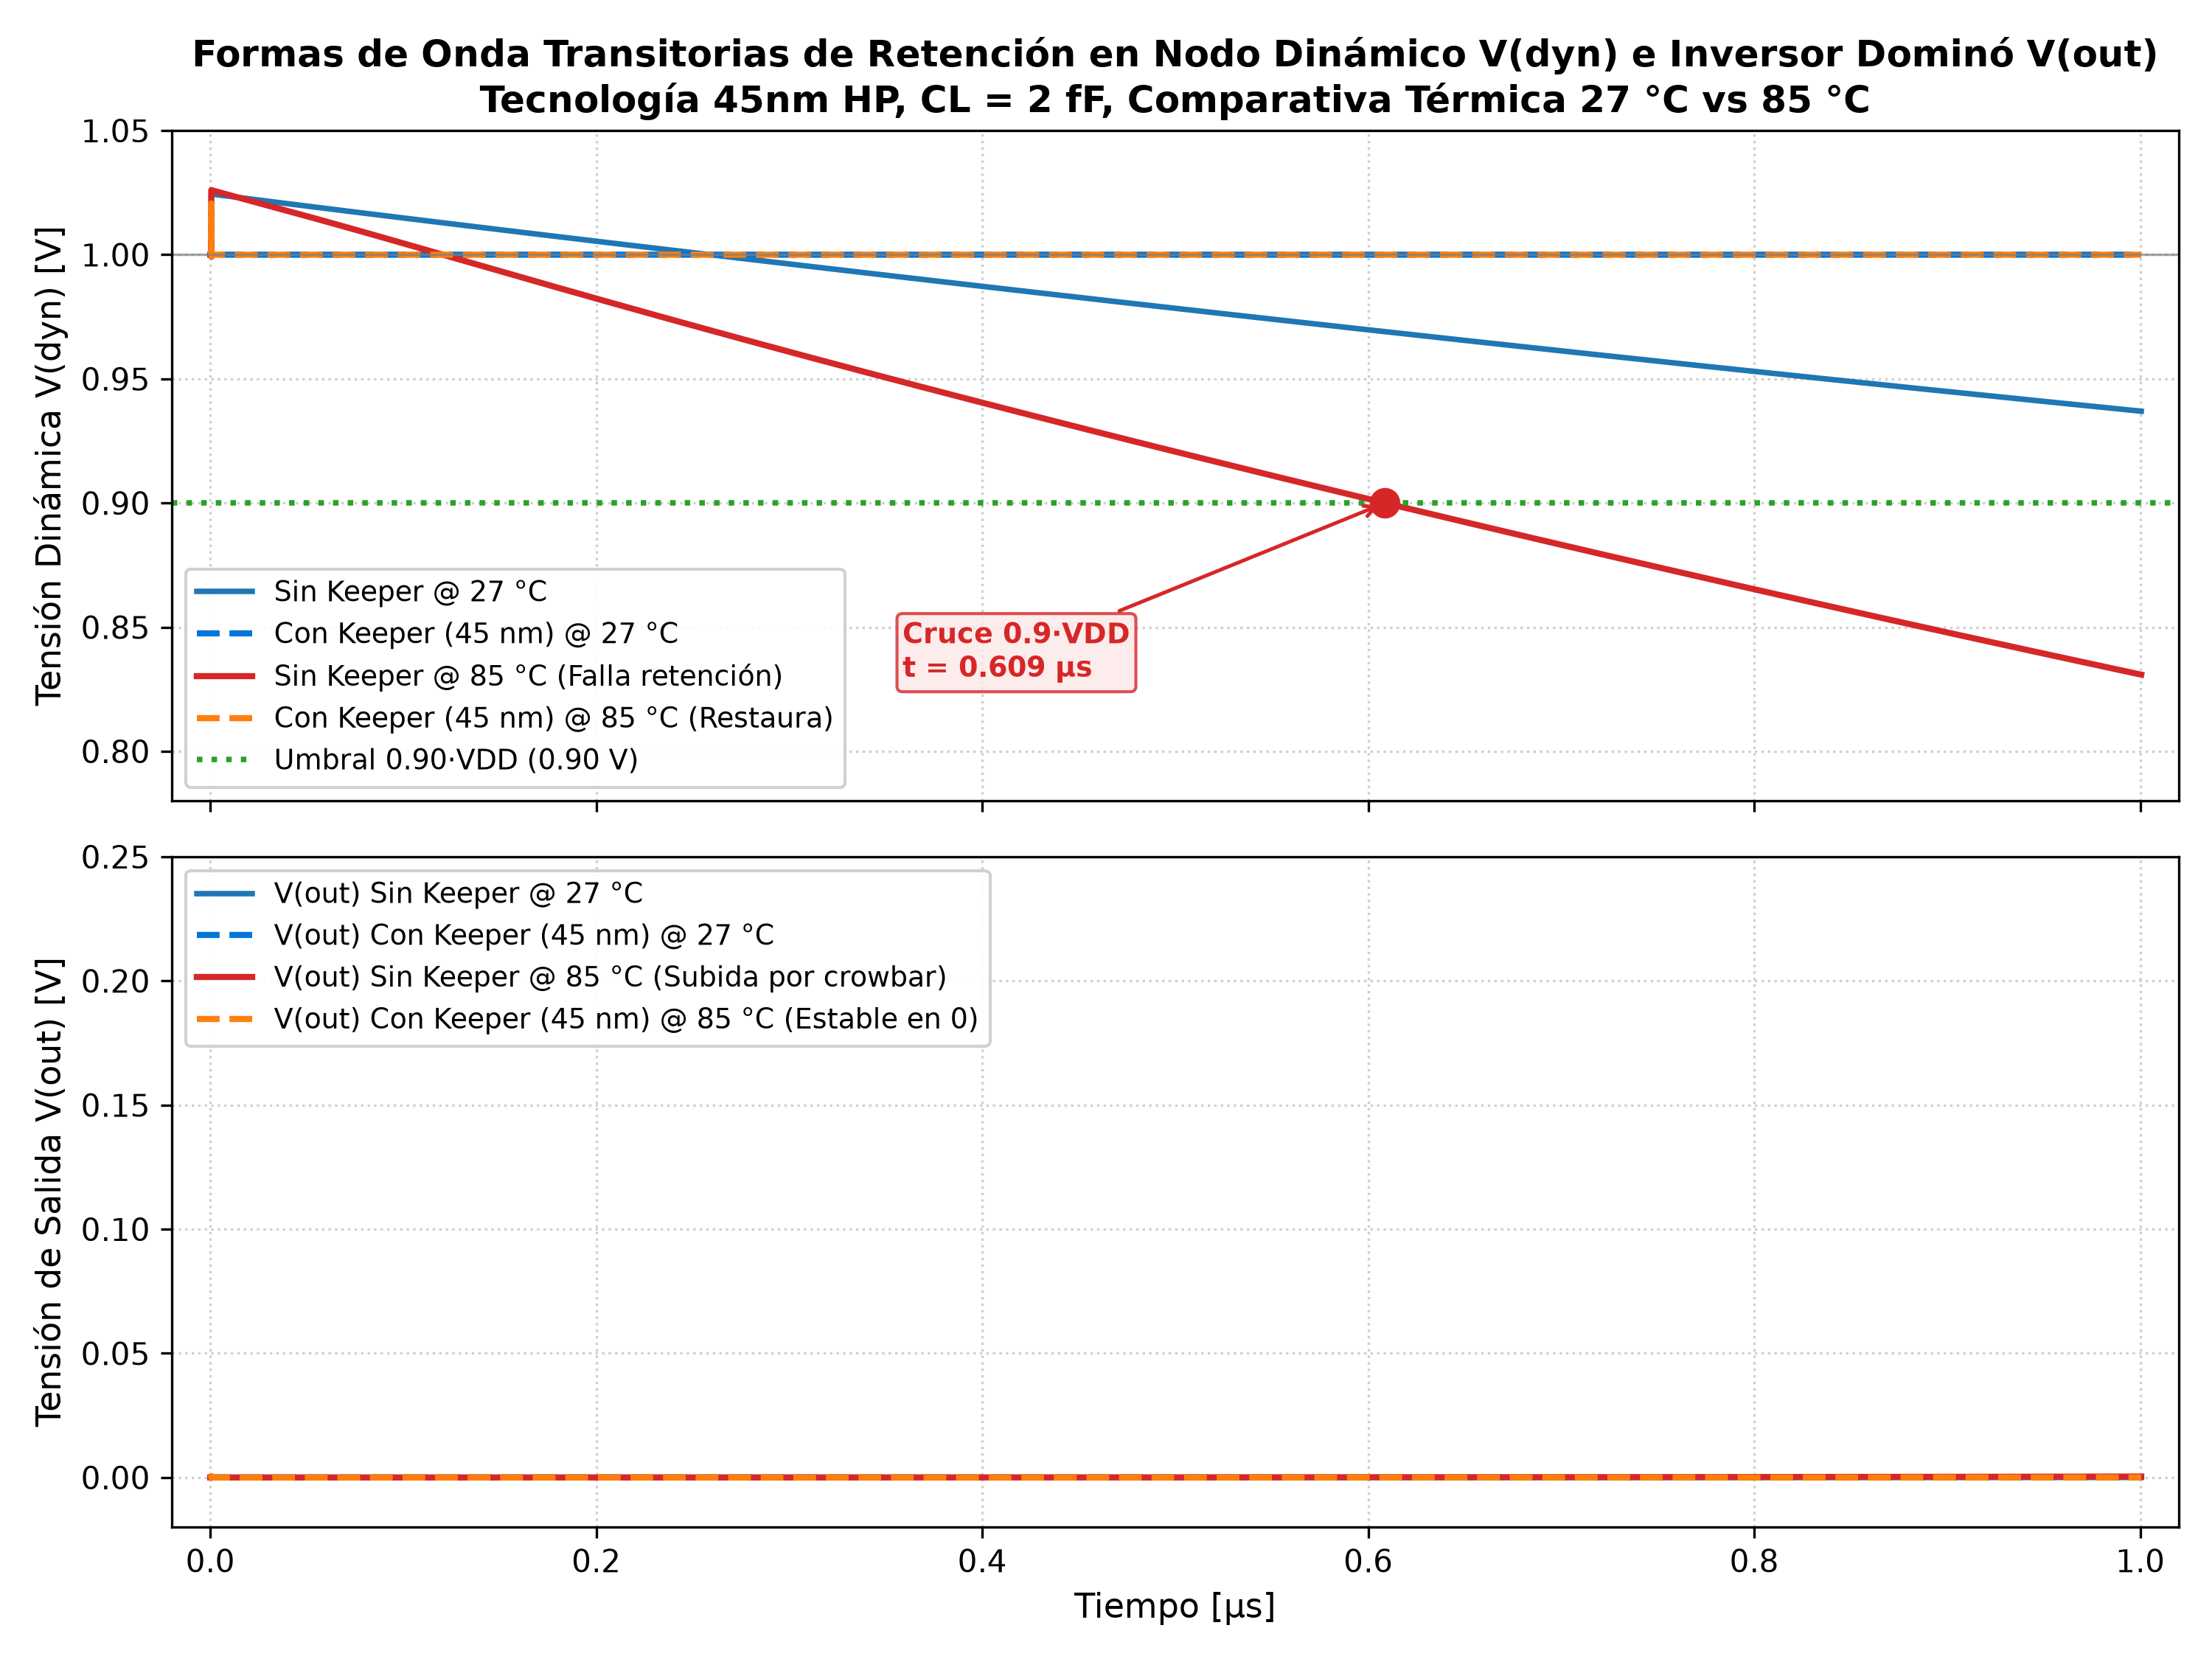
\includegraphics[width=0.62\linewidth]{figuras/fig1_act3_retencion_formas_onda.png}
  \caption[Formas de onda transitorias de retención en el nodo dinámico]{Formas de onda transitorias de retención en el nodo $dyn$ y salida $out$ durante $1.0\,\mu\text{s}$ en 45\,nm HP ($C_L=2\,\text{fF}$), contrastando la respuesta sin keeper a $27^\circ\text{C}$ y $85^\circ\text{C}$ frente al circuito con keeper ($W_{kp}=45\,\text{nm}$).}
  \label{fig:retencion_formas_onda}
\end{figure}

Las curvas transitorias se presentan en la Figura~\ref{fig:retencion_formas_onda}. En ausencia de keeper:
\begin{itemize}[leftmargin=1.4em,itemsep=0.15em]
  \item \textbf{A temperatura ambiente ($27^\circ\text{C}$):} La tensión dinámica evoluciona entre los extremos medidos $V_{dyn}(t_0 = 10.0\,\text{ns}) = 1.023497\,\text{V}$ y $V_{dyn}(t_1 = 1000.520\,\text{ns}) = 0.936959\,\text{V}$, registrando una caída total de $\Delta V_{dyn} = -86.538\,\text{mV}$. El circuito \textbf{cumple holgadamente} el criterio estricto de la guía ($V_{dyn} > 0.90\,V_{DD} = 0.90\,\text{V}$) durante todo el intervalo de $1\,\mu\text{s}$.
  \item \textbf{A alta temperatura ($85^\circ\text{C}$):} El incremento térmico de las corrientes de fuga acelera el drenaje de portadores, con extremos reales $V_{dyn}(t_0) = 1.023977\,\text{V}$ y $V_{dyn}(t_1) = 0.830869\,\text{V}$ ($\Delta V_{dyn} = -193.108\,\text{mV}$). La tensión cruza el umbral de $0.90\,V_{DD} = 0.90\,\text{V}$ en un tiempo absoluto transitorio de $t_{\text{cross}} = 608.69\,\text{ns}$, lo que equivale a un tiempo de retención neto en evaluación de $t_{\text{hold}} = t_{\text{cross}} - t_{\text{eval\_start}} = 608.17\,\text{ns}$ (con $t_{\text{eval\_start}} = 0.52\,\text{ns}$), \textbf{incumpliendo el criterio estricto de retención} frente a la ventana de evaluación ensayada de $1.0\,\mu\text{s}$ ($T_{\text{ret}} = 1000.0\,\text{ns}$). No obstante, dado que $V_{dyn}(1\,\mu\text{s}) = 0.831\,\text{V}$ se mantiene por encima de la tensión de conmutación del inversor dominó ($V_M \approx 0.50\,\text{V}$), la salida permanece estable en $out = 0\,\text{V}$, sin manifestar falla lógica funcional dentro de la ventana de $1\,\mu\text{s}$.
\end{itemize}

\noindent\textbf{Acoplamiento Capacitivo en $t_0$:} En ambas temperaturas, $V_{dyn}(t_0)$ supera ligeramente la tensión de alimentación nominal ($1.0235\,\text{V}$ y $1.0240\,\text{V}$). Este fenómeno responde al acoplamiento capacitivo (\textit{clock feedthrough} / \textit{bootstrap}) transmitido por la capacitancia de solapamiento compuerta-drenaje $C_{gd}(M_p)$ durante la transición ascendente del reloj ($CLK: 0 \to 1\,\text{V}$); por ende, no debe asumirse artificialmente $V_{dyn}(t_0) = 1.000\,\text{V}$.

\subsubsection{Conciliación Metodológica de Capacitancias Nodal y Aparente}
En la formulación analítica previa se estimó una capacitancia parásita estática en pequeña señal de $C_{\text{par}} \approx 0.65\,\text{fF}$, resultando en $C_{dyn,\text{teor}} \approx C_L + C_{\text{par}} \approx 2.65\,\text{fF}$. Sin embargo, la integración numérica directa en gran señal revela una dinámica aparente distinta:
\begin{enumerate}[leftmargin=1.4em,itemsep=0.12em]
  \item \textbf{Parámetro circuital explícito ($C_L = 2.0\,\text{fF}$):} La integración temporal de la corriente terminal $I(C_L)$ en el archivo RAW durante la ventana $\Delta t = 990.520\,\text{ns}$ arroja $\langle I(C_L) \rangle = -174.732\,\text{pA}$ a $27^\circ\text{C}$ y $-389.913\,\text{pA}$ a $85^\circ\text{C}$, coincidente a seis cifras significativas con $C_L \frac{\Delta V_{dyn}}{\Delta t}$. El capacitor físico concentra el 91.5\% de la corriente total de descarga.
  \item \textbf{Capacitancia dinámica aparente inferida ($C_{\text{eff}}$):} A partir del balance integral de cargas con la corriente terminal neta demandada por los semiconductores ($\langle I_{\text{net,dev}} \rangle$):
  \begin{equation}
    C_{\text{eff}} \equiv \frac{\langle I_{\text{net,dev}} \rangle \cdot \Delta t}{|\Delta V_{dyn}|} = 
    \begin{cases}
      \dfrac{191.021\,\text{pA} \times 990.520\,\text{ns}}{86.53768\,\text{mV}} = \mathbf{2.18645\,\text{fF}} & (27^\circ\text{C}) \\[1em]
      \dfrac{425.281\,\text{pA} \times 990.520\,\text{ns}}{193.10813\,\text{mV}} = \mathbf{2.18142\,\text{fF}} & (85^\circ\text{C})
    \end{cases}
    \label{eq:ceff}
  \end{equation}
  \item \textbf{Capacitancia parásita aparente ($C_{\text{par}}$):} Se deduce algebraicamente para cerrar la ley de Kirchhoff:
  \begin{equation}
    C_{\text{par,aparente}} \equiv C_{\text{eff}} - C_L = 
    \begin{cases}
      0.18645\,\text{fF} & (27^\circ\text{C}) \\
      0.18142\,\text{fF} & (85^\circ\text{C})
    \end{cases}
  \end{equation}
  suministrando el remanente dinámico de $+16.29\,\text{pA}$ a $27^\circ\text{C}$ y $+35.37\,\text{pA}$ a $85^\circ\text{C}$.
\end{enumerate}

\noindent\textbf{Interpretación Física Plausible:} La reducción de la capacitancia parásita efectiva frente a la predicción estática lineal ($0.186\,\text{fF}$ vs $0.65\,\text{fF}$) se fundamenta en las condiciones de polarización dinámica durante la retención:
\begin{itemize}[leftmargin=1.4em,itemsep=0.1em]
  \item Al mantenerse $V_{dyn} \approx 1.0\,\text{V}$, el transistor PMOS del inversor ($M_{pi}$) opera con $V_{GS} = V(dyn) - V_{DD} \approx 0\,\text{V}$, situándose en régimen de agotamiento/subumbral. Su capacitancia de compuerta cae desde el valor de inversión fuerte ($W L C_{ox} \approx 0.28\,\text{fF}$) hacia la fracción residual de solapamiento ($C_{ov} \ll C_{ox}$).
  \item Las uniones $p\text{-}n$ de difusión conectadas a $dyn$ se encuentran polarizadas en reversa plena ($V_R = 1.0\,\text{V}$), lo que ensancha la zona de carga espacial y disminuye la capacitancia de unión en aproximadamente un 30\% respecto al valor a tensión nula.
\end{itemize}
$C_{\text{eff}}$ y $C_{\text{par}}$ representan parámetros aparentes derivados de la relación integral de carga y no deben interpretarse como una extracción física aislada e independiente de cada parásito circuital.

\subsection{Descomposición de Componentes de Fuga y Balance Nodal}
Para dilucidar los mecanismos físicos dominantes en la descarga del nodo flotante, se aplicó la ley de corrientes de Kirchhoff (KCL) sobre los terminales conectados a $dyn$ en la ventana de retención:
\begin{equation}
  \langle I_s(M_1) \rangle + \langle I_d(M_p) \rangle + \langle I_g(M_{pi}) \rangle + \langle I_g(M_{ni}) \rangle + \langle I(C_L) \rangle + \langle I(C_{\text{par}}) \rangle = 0
  \label{eq:kcl_dyn}
\end{equation}

Los resultados cuantitativos se consolidan en la Tabla~\ref{tab:balance_fugas}.

% Tabla de balance nodal y corrientes terminales de fuga en dyn - Actividad 3
% Fuentes: dc_fugas_nmos_pdn, dc_fugas_compuerta, raw/nand3_retencion_sin_keeper
\begin{table}[htbp]
\centering
\scriptsize
\setlength{\tabcolsep}{3.5pt}
\caption[Balance nodal promedio de corrientes terminales en el nodo dinámico]{Balance nodal promedio de corrientes terminales en el nodo $dyn$ durante la ventana de retención ($t \in [10.0\,\text{ns},\, 1000.52\,\text{ns}]$, $\Delta t = 990.52\,\text{ns}$, 45\,nm HP).}
\label{tab:balance_fugas}
\begin{tabularx}{\linewidth}{@{}>{\RaggedRight\arraybackslash}p{3.2cm} c c c >{\RaggedRight\arraybackslash}X@{}}
\toprule
\textbf{Rama / Terminal de Conexión} & \textbf{$27^\circ\text{C}$} & \textbf{$85^\circ\text{C}$} & \textbf{Factor Térmico} & \textbf{Mecanismo y Rol Físico en el Nodo $dyn$} \\
\midrule
Drenaje hacia PDN Footed, $\langle I_s(M_1) \rangle$ & $+110.53\,\text{pA}$ & $+430.89\,\text{pA}$ & $3.90\times$ & Subumbral con DIBL y uniones reverse en la pila apilada ($V_{SB} \in [0.1, 0.25]\,\text{V}$). \\
Inyección de Precarga, $\langle I_d(M_p) \rangle$ & $-12.26\,\text{pA}$ & $-56.08\,\text{pA}$ & $4.57\times$ & PMOS en corte ($V_{GS}=0\,\text{V}, V_{DS} \approx 0\,\text{V}$); inyecta carga reconstitutiva hacia $dyn$. \\
Compuerta PMOS Inversor, $\langle I_g(M_{pi}) \rangle$ & $+76.31\,\text{pA}$ & $+49.86\,\text{pA}$ & $0.65\times$ & Túnel de compuerta directo ($V_{GD} \approx 1.0\,\text{V}$); drena portadores de $dyn$. \\
Compuerta NMOS Inversor, $\langle I_g(M_{ni}) \rangle$ & $+16.44\,\text{pA}$ & $+0.61\,\text{pA}$ & $0.04\times$ & Túnel de compuerta NMOS ($V_{GS} \approx 1.0\,\text{V}$ en $t_0$, decae al polarizarse). \\
\midrule
\multicolumn{5}{@{}l@{}}{\textbf{Partición de Corriente Saliente de $dyn$ (Antes de Descontar Precarga $M_p$)}} \\
Rama PDN / Inversor Dominó & 54.4\% / 45.6\% & 89.5\% / 10.5\% & --- & A $85^\circ\text{C}$, el crecimiento subumbral ($3.90\times$) domina sobre el túnel. \\
\midrule
Corriente Neta Demandada, $\langle I_{\text{net,dev}} \rangle$ & $+191.02\,\text{pA}$ & $+425.28\,\text{pA}$ & $2.23\times$ & Suma algebraica neta de semiconductores ($\sum I_{\text{terminales}}$). \\
Corriente Capacitor Carga, $\langle I(C_L) \rangle$ & $-174.73\,\text{pA}$ & $-389.91\,\text{pA}$ & $2.23\times$ & Integración directa de $C_L=2.0\,\text{fF}$ en RAW; suministra el 91.5\% de la descarga. \\
Remanente Parásito Dinámico & $+16.29\,\text{pA}$ & $+35.37\,\text{pA}$ & $2.17\times$ & Suministrado por la capacitancia parásita aparente ($C_{\text{par}} \approx 0.186\,\text{fF}$). \\
\midrule
Compuerta Externa NMOS $M_1$, $I_g(M_1)$ & $-41.604\,\text{pA}$ & $-41.604\,\text{pA}$ & $1.00\times$ & Corriente terminal supplied por la entrada externa $a$; no descarga el nodo $dyn$. \\
\bottomrule
\end{tabularx}
\end{table}


\begin{enumerate}[leftmargin=1.4em,itemsep=0.15em]
  \item \textbf{Drenaje hacia la PDN Footed ($\langle I_s(M_1) \rangle$):} Es la vía principal de extracción de carga hacia tierra, integrando la corriente subumbral modulada por DIBL, las corrientes de unión reversa y el túnel acoplado compuerta-fuente a lo largo de la pila de 4 NMOS. A $27^\circ\text{C}$ promedia $+110.53\,\text{pA}$, incrementándose a $+430.89\,\text{pA}$ a $85^\circ\text{C}$ (factor de $\mathbf{3.90\times}$).
  \item \textbf{Inyección Reconstitutiva de Precarga ($\langle I_d(M_p) \rangle$):} Dado que $M_p$ está cortado pero polarizado con $V_{DS} \approx 0 \to 0.17\,\text{V}$, drena una corriente negativa ($-12.26\,\text{pA}$ a $27^\circ\text{C}$ y $-56.08\,\text{pA}$ a $85^\circ\text{C}$) que inyecta portadores desde $V_{DD}$ hacia $dyn$, atenuando levemente la descarga neta.
  \item \textbf{Fugas de Compuerta del Inversor Dominó ($\langle I_g(M_{pi}) \rangle, \langle I_g(M_{ni}) \rangle$):} El PMOS $M_{pi}$ presenta un campo transversal intenso en su compuerta ($V_{GD} \approx 1.0\,\text{V}$), absorbiendo $+76.31\,\text{pA}$ a $27^\circ\text{C}$ por efecto túnel directo (\textit{direct gate tunneling}). El NMOS $M_{ni}$ aporta $+16.44\,\text{pA}$ a $27^\circ\text{C}$.
  \item \textbf{Fuga de Compuerta Externa de $M_1$ ($I_g(M_1) = -41.604\,\text{pA}$):} Caracterizada en banco DC bajo $V_a = 0\,\text{V}, V_{dyn} = 1.0\,\text{V}$. Esta corriente es provista directamente por el generador de la entrada lógica $a$; cualquier componente de acoplamiento interno hacia el canal ya se encuentra físicamente integrada en la corriente de fuente $I_s(M_1)$. Por rigor metodológico, \textbf{no debe sumarse independientemente por segunda vez} al balance nodal de $dyn$.
  \item \textbf{Partición de Ramas de Descarga:} Antes de compensar la inyección de precarga, la corriente saliente de $dyn$ se distribuye:
  \begin{itemize}[leftmargin=1.2em,itemsep=0.08em]
    \item A $27^\circ\text{C}$: 54.4\% hacia la PDN ($110.53\,\text{pA}$) frente a 45.6\% hacia las compuertas del inversor ($92.75\,\text{pA}$).
    \item A $85^\circ\text{C}$: 89.5\% hacia la PDN ($430.89\,\text{pA}$) frente a 10.5\% hacia las compuertas ($50.47\,\text{pA}$).
  \end{itemize}
  Estas proporciones describen estrictamente el reparto entre ramas circuitales y no constituyen una descomposición matemática aislada entre portadores subumbral puros y corriente túnel.
\end{enumerate}

\subsubsection{Investigación Experimental de GIDL por Ablación Controlada}
Para aislar la corriente de fuga inducida por drenador (\textit{Gate-Induced Drain Leakage}, GIDL), se contrastó el modelo canónico 45\,nm HP frente a un modelo modificado en la librería auxiliar \texttt{modelos/ptm45hp\_aux.lib} donde se forzó el parámetro \texttt{agidl = 0.0}. 

Bajo las condiciones operativas de retención ($V_{DS} = 1.0\,\text{V}$, $V_{GS} = 0\,\text{V}$, $V_{SB} = 0\,\text{V}$), la diferencia en corriente de drenador resultó nula dentro de la precisión numérica del simulador ($\Delta I_D = 0.0\,\text{A}$), mientras que la corriente de sustrato registró una variación infinitesimal $|\Delta I_B| \sim 2.5 \times 10^{-20}\,\text{A}$, indistinguible del ruido numérico de punto flotante. Se concluye que la contribución GIDL no tiene impacto práctico medible en la tasa de descarga del nodo $dyn$ bajo la polarización analizada, sin que ello autorice a postular una inexistencia física absoluta del fenómeno en regímenes de campo ultra-intenso.

\subsection{Dependencia Térmica y Comparación Tecnológica Tri-Nodo}
El modelo analítico clásico predice que la corriente subumbral escala exponencialmente con la temperatura:
\begin{equation}
  I_{sub}(T) \propto \left(\frac{k T}{q}\right)^2 \exp\left(\frac{V_{GS} - V_{th}(T)}{n \, (k T / q)}\right)
  \label{eq:isub_temp}
\end{equation}
con un corrimiento lineal del voltaje de umbral aproximado tradicionalmente en la literatura como $\frac{d V_{th}}{d T} \approx -1.0\,\text{mV/}^\circ\text{C}$. En el modelo PTM BSIM4 implementado, la modulación térmica responde al parámetro intrínseco $k_{t1} = -0.11\,\text{V}$, derivando una pendiente analítica de:
\begin{equation}
  \frac{\Delta V_{th}}{\Delta T} = \frac{k_{t1}}{T_{\text{nom}}} = \frac{-0.11\,\text{V}}{300.15\,\text{K}} \approx -0.366\,\text{mV/}^\circ\text{C} \implies \Delta V_{th}(85^\circ\text{C} - 27^\circ\text{C}) \approx -21.2\,\text{mV}
\end{equation}
la cual exhibe una atenuación intrínseca más moderada frente a la regla heurística de $-1.0\,\text{mV/}^\circ\text{C}$ ($\Delta V_{th} \approx -58\,\text{mV}$).

\noindent\textbf{Factores Térmicos Multi-Nivel:}
\begin{itemize}[leftmargin=1.4em,itemsep=0.12em]
  \item \textbf{Transistor NMOS aislado en banco DC ($V_{DS} = 1.0\,\text{V}$):} Al elevar la temperatura de $27^\circ\text{C}$ a $85^\circ\text{C}$, el factor térmico se gradúa según el potencial de cuerpo: $3.13\times$ para $V_{SB} = 0.0\,\text{V}$ ($5.51 \to 17.25\,\text{nA}$), $4.13\times$ para $V_{SB} = 0.3\,\text{V}$ ($0.84 \to 3.49\,\text{nA}$), y $4.63\times$ para $V_{SB} = 0.6\,\text{V}$ ($0.18 \to 0.83\,\text{nA}$).
  \item \textbf{Red Pull-Down completa in situ:} La corriente terminal $I_s(M_1)$ pasa de $110.53\,\text{pA}$ a $430.89\,\text{pA}$, reflejando un factor térmico terminal de $\mathbf{3.90\times}$. Este factor se sitúa entre los valores medidos en banco DC a $V_{SB}=0.0$ y $0.3\,\text{V}$; es compatible con la modulación por efecto cuerpo y apilamiento, pero no determina por sí solo las tensiones internas $n_1,n_2,n_3$ ni constituye una cota universal para la red.
\end{itemize}

\subsubsection{Consolidación Tecnológica: 45~nm HP, 45~nm LP y 130~nm Bulk}
Se replicó el ensayo de retención sobre tres plataformas semiconductoras distintas según la tarea~3 de la guía. La Tabla~\ref{tab:retencion_tecnologica} resume las métricas cuantitativas, y la Figura~\ref{fig:consolidacion_tecnologica} exhibe las curvas de retención normalizadas frente al ancho del keeper $W_{kp}$.

% Tabla de consolidacion tecnologica de retencion - Actividad 3
% Fuentes: act3_consolidacion_tecnologica.json, logs canonicos de retencion
\begin{table}[htbp]
\centering
\footnotesize
\caption[Consolidación tecnológica tri-nodo de retención sin keeper]{Consolidación tecnológica tri-nodo de retención en el nodo dinámico sin keeper ($T_{\text{stop}}=1.0\,\mu\text{s}$, $C_L=2.0\,\text{fF}$, reloj detenido en evaluación con PDN abierta $A=B=C=0$).}
\label{tab:retencion_tecnologica}
\begin{tabularx}{\linewidth}{@{}>{\RaggedRight\arraybackslash}p{2.5cm} c c c c c >{\RaggedRight\arraybackslash}X@{}}
\toprule
\textbf{Tecnología / Proceso} & \textbf{Temp.} & \textbf{$V_{DD}$} & \textbf{$V_{dyn}(1\,\mu\text{s})$} & \textbf{$t_{\text{hold}}$ [$t_{\text{cross}}$]\textsuperscript{*}} & \textbf{$W_{kp}$ mín. ensayado} & \textbf{Estado y Diagnóstico Físico} \\
\midrule
45\,nm HP & $27^\circ\text{C}$ & 1.0\,V & 0.9370\,V & $>1.0\,\mu\text{s}$ (Cens.) & No req. & \textbf{CUMPLE} ($V_{dyn} > 0.90\,V_{DD}$). Fuga subumbral moderada. \\
45\,nm HP & $85^\circ\text{C}$ & 1.0\,V & 0.8309\,V & 608.17\,ns [608.69\,ns] & 10.5\,nm (malla fina) & \textbf{FALLA} criterio $0.90\,V_{DD}$; \textbf{CUMPLE} nivel lógico ($V_{dyn} > V_M \approx 0.50\,\text{V}$). \\
\midrule
45\,nm LP & $27^\circ\text{C}$ & 1.1\,V & 1.1275\,V & $>1.0\,\mu\text{s}$ (Cens.) & No req. & \textbf{CUMPLE}. Óxido grueso ($t_{oxe}=1.8\,\text{nm}$) y $V_{th}$ elevado suprimen fuga. \\
45\,nm LP & $85^\circ\text{C}$ & 1.1\,V & 1.1257\,V & $>1.0\,\mu\text{s}$ (Cens.) & No req. & \textbf{CUMPLE}. Retención robusta sin keeper ($I_{leak} \sim 7\,\text{pA}$). \\
\midrule
130\,nm Bulk & $27^\circ\text{C}$ & 1.3\,V & 1.0178\,V & 318.31\,ns [318.83\,ns] & 15.0\,nm & \textbf{FALLA} criterio $0.90\,V_{DD}$ (1.17\,V); \textbf{CUMPLE} lógico ($V_{dyn} > V_M \approx 0.60\,\text{V}$). \\
130\,nm Bulk & $85^\circ\text{C}$ & 1.3\,V & 0.8770\,V & 167.53\,ns [168.05\,ns] & 15.0\,nm & \textbf{FALLA} estricto; \textbf{CUMPLE} lógico. Requiere keeper por fuga de canal ancho. \\
\midrule
\multicolumn{7}{@{}p{\linewidth}@{}}{\footnotesize \textsuperscript{*} $t_{\text{hold}} \equiv t_{\text{cross}} - t_{\text{eval\_start}}$, con $t_{\text{eval\_start}} = 0.52\,\text{ns}$ y $t_{\text{cross}}$ medido desde el inicio del transitorio hasta el cruce con $0.90\,V_{DD}$. La duración neta de evaluación ensayada es de $T_{\text{ret}} = 1000.0\,\text{ns} = 1.0\,\mu\text{s}$ ($T_{\text{stop}} = 1000.52\,\text{ns}$). Casos sin cruce se reportan formalmente censurados ($t_{\text{hold}} > 1.0\,\mu\text{s}$). La ventana para el balance de corrientes y cálculo de $C_{\text{eff}}$ emplea el intervalo cuasi-estacionario $t \in [10.0\,\text{ns},\, 1000.52\,\text{ns}]$ ($\Delta t = 990.52\,\text{ns}$) para excluir el acoplamiento transitorio del reloj ($CLK: 0 \to 1\,\text{V}$). $W_{kp}$ corresponde al menor ancho evaluado en la malla de simulación que satisface retención, no a una regla DRC universal.} \\
\bottomrule
\end{tabularx}
\end{table}


\begin{figure}[htbp]
  \centering
  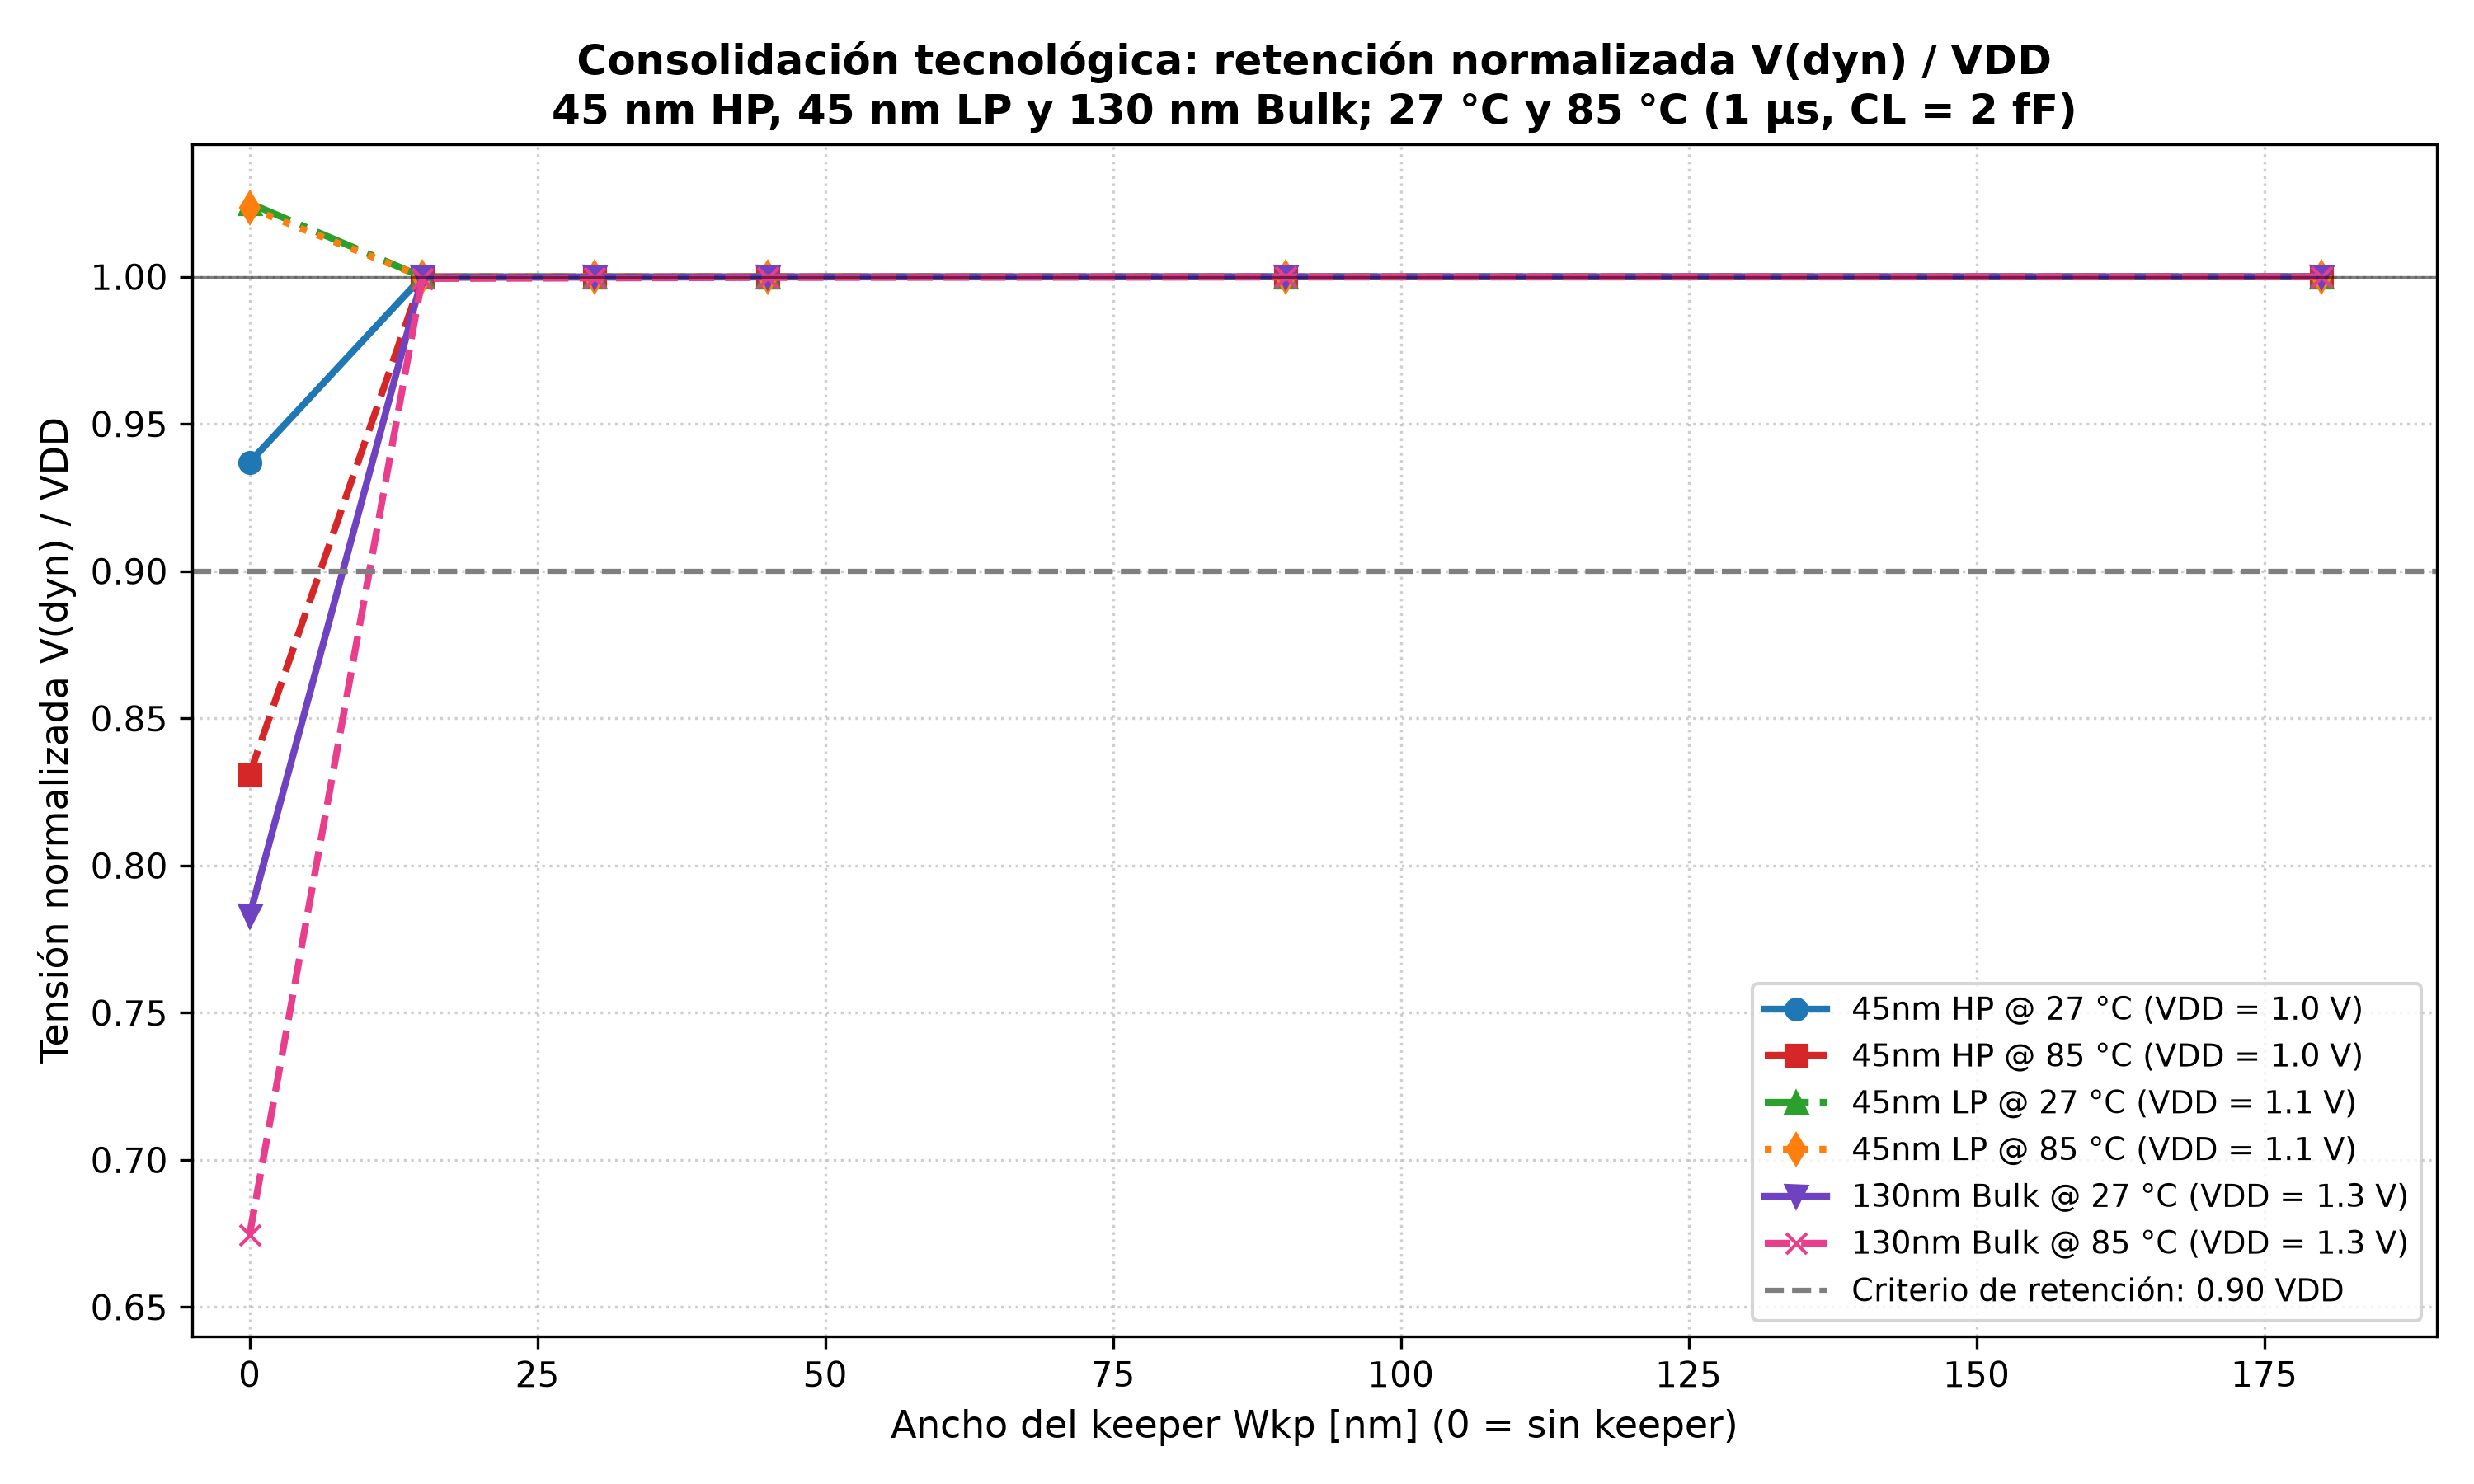
\includegraphics[width=0.78\linewidth]{figuras/fig2_act3_consolidacion_hp_lp_130.png}
  \caption[Consolidación tecnológica tri-nodo de retención]{Tensión normalizada de retención $V_{dyn}(1\,\mu\text{s})/V_{DD}$ en función de $W_{kp}$ para 45\,nm HP, 45\,nm LP y 130\,nm Bulk a $27^\circ\text{C}$ y $85^\circ\text{C}$ ($T_{\text{stop}}=1\,\mu\text{s}$).}
  \label{fig:consolidacion_tecnologica}
\end{figure}

\begin{enumerate}[leftmargin=1.4em,itemsep=0.15em]
  \item \textbf{Tecnología 45\,nm Low Power (LP, $V_{DD}=1.1\,\text{V}$):} Exhibe menor caída del nodo en este ensayo. El óxido de compuerta más grueso ($t_{oxe} = 1.80\,\text{nm}$) y el umbral nominal mayor ($V_{th0} \approx 0.62\,\text{V}$) contribuyen a reducir las fugas; a $85^\circ\text{C}$ se midieron $7.06\,\text{pA}$ de corriente media de alimentación y $3.40\,\text{pA}$ en la rama PDN (magnitudes distintas). El nodo termina en $1.1275\,\text{V}$ a $27^\circ\text{C}$ y $1.1257\,\text{V}$ a $85^\circ\text{C}$; la sobretensión inicial por acoplamiento no equivale a ganancia de carga neta. No requiere keeper para satisfacer el criterio en la ventana simulada de $1\,\mu\text{s}$ ($t_{\text{hold}} > 1.0\,\mu\text{s}$, formalmente censurado en $T_{\text{ret}} = 1000.0\,\text{ns}$).
  \item \textbf{Tecnología 130\,nm Bulk ($V_{DD}=1.3\,\text{V}$):} En la configuración ensayada, con $W_n = 3 \times 260\,\text{nm} = 780\,\text{nm}$ y $C_L=2\,\text{fF}$, la red presenta una descarga apreciable: cruza el umbral de $0.90\,V_{DD} = 1.17\,\text{V}$ en $t_{\text{cross}} = 318.83\,\text{ns}$ ($t_{\text{hold}} = 318.31\,\text{ns}$) a $27^\circ\text{C}$ y en $t_{\text{cross}} = 168.05\,\text{ns}$ ($t_{\text{hold}} = 167.53\,\text{ns}$) a $85^\circ\text{C}$. A $85^\circ\text{C}$ termina en $0.8770\,\text{V}$; aunque la salida no conmuta espuriamente ($V_M \approx 0.60\,\text{V}$), \textbf{falla el criterio estricto de retención}. El ancho $W_{kp} = 15.0\,\text{nm}$ es el menor punto ensayado en la malla de simulación que lo satisface, no un límite físico universal intrínseco. Asimismo, la comparación entre nodos involucra variaciones simultáneas en $W_n$ y $V_{DD}$, por lo que no aísla de forma exclusiva el efecto intrínseco de la tecnología.
\end{enumerate}

\noindent\textbf{Efecto del Keeper en 45\,nm HP:} La adición de un transistor PMOS gobernado por la salida restauradora $out$ sostiene el nodo flotante. En los anchos discretos ensayados entre $10.5$ y $180\,\text{nm}$ (incluido el punto de la guía $W_{kp}=22\,\text{nm}$), se obtiene $V_{dyn}(1\,\mu\text{s}) > 0.9999\,\text{V}$ a ambas temperaturas. No se ha demostrado retención ilimitada ni un ancho mínimo continuo. El valor $W_{kp} = 10.5\,\text{nm}$ corresponde a la cota inferior evaluada en la malla de simulación fina que converge y satisface retención; en el modelo BSIM4 PTM 45\,nm, el parámetro intrínseco $W_{\text{int}} = 5\,\text{nm}$ impone un ancho eléctrico efectivo $W_{\text{eff}} = W - 2 W_{\text{int}} = W - 10\,\text{nm}$, por lo que valores $W \le 10\,\text{nm}$ (e.g., $W_{kp} = 1\,\text{nm}$) generan $W_{\text{eff}} \le 0$ y provocan el aborto numérico inmediato del simulador. Dicho límite numérico del modelo no debe confundirse con una regla de diseño de fundición (DRC).

\subsection{Evaluación de Contención y Penalización de Velocidad en Evaluación Activa}
Aunque un keeper suficientemente dimensionado compensa la descarga por fugas durante la ventana simulada, su presencia introduce el fenómeno de \textbf{contención de corriente} (\textit{keeper contention}) durante la fase de evaluación activa ($CLK=1, A=B=C=1$). En el instante en que la PDN comienza a descargar el nodo dinámico, la salida del inversor dominó aún permanece en nivel bajo ($out = 0\,\text{V}$), manteniendo al keeper encendido. El keeper disputa corriente con los transistores NMOS en serie, inyectando portadores desde $V_{DD}$ y demorando la conmutación hacia tierra.

Conforme a la tarea~4 de la guía, se define una razón geométrica de dimensionamiento relativo $r$ que normaliza el ancho del keeper respecto al ancho equivalente de la red de descarga (PDN). En la tecnología 45\,nm HP, el ancho unitario de referencia es $W_{n,\text{unit}} = 90\,\text{nm}$. Para compensar la degradación por apilamiento, los transistores de la PDN se dimensionan a $W_{n,\text{stack}} = 3 \times W_{n,\text{unit}} = 270\,\text{nm}$. Dado que la PDN footed consta de 4 transistores NMOS en serie (tres de la compuerta lógica $M_1, M_2, M_3$ y el transistor footed de reloj $M_f$, todos con $W_n = 270\,\text{nm}$ y $L_n = 45\,\text{nm}$), el ancho equivalente de la pila en serie se aproxima geométricamente por:
\begin{equation}
  W_{PDN,eq} \approx \frac{W_{n,\text{stack}}}{4} = \frac{270\,\text{nm}}{4} = 67.5\,\text{nm}
\end{equation}
Adoptando longitudes nominales de canal idénticas ($L_p = L_n = 45\,\text{nm}$), la razón de aspecto de dimensionamiento resulta:
\begin{equation}
  r \equiv \frac{(W/L)_{kp}}{(W/L)_{PDN,eq}} = \frac{W_{kp}/L_p}{W_{PDN,eq}/L_n} = \frac{W_{kp}/45\,\text{nm}}{67.5\,\text{nm}/45\,\text{nm}} = \frac{W_{kp}}{67.5\,\text{nm}}
  \label{eq:ratio_r}
\end{equation}
Es fundamental precisar que $r$ constituye una métrica heurística y puramente geométrica de dimensionamiento relativo adoptada según la guía docente, y \textbf{no} un cómputo riguroso de la resistencia efectiva de conmutación o una extracción dinámica de pequeña señal (la cual se ve fuertemente afectada por la saturación de velocidad, el efecto de cuerpo variable $V_{SB} > 0$ a lo largo de la pila y las tensiones transitorias de sobremarcha $V_{GS} - V_{th}$).
La rúbrica docente fija como cota estricta que la penalización en el retardo de evaluación no debe exceder el 10\%:
\begin{equation}
  \text{Penalización } \Delta t_{pHL} \equiv \frac{t_{pHL,dyn}(W_{kp}) - t_{pHL,\text{base}}}{t_{pHL,\text{base}}} \times 100\% < 10.0\%
  \label{eq:cota_contencion}
\end{equation}
donde el retardo de referencia sin keeper a $85^\circ\text{C}$ es $t_{pHL,\text{base}} = 31.80\,\text{ps}$ en 45\,nm HP y $105.74\,\text{ps}$ en 45\,nm LP.

% Tabla de contencion y penalizacion de retardo en evaluacion - Actividad 3
% Fuentes: act3_contencion_metricas.json, act3_conciliacion_a3_5_1.json, act3_descomposicion_causal.json
\begin{table}[htbp]
\centering
\footnotesize
\caption[Penalización de velocidad por contención del keeper en evaluación activa]{Penalización de velocidad en evaluación activa ($A=B=C=1$) bajo peor caso térmico ($85^\circ\text{C}$, $C_L=2.0\,\text{fF}$, $C_{out}=1.0\,\text{fF}$).}
\label{tab:contencion}
\begin{tabularx}{\linewidth}{@{}>{\RaggedRight\arraybackslash}p{3.2cm} c c c c >{\RaggedRight\arraybackslash}X@{}}
\toprule
\textbf{Arquitectura / Configuración} & \textbf{$W_{kp}$} & \textbf{$r = \frac{W_{kp}}{67.5\,\text{nm}}$} & \textbf{$t_{pHL,dyn}$} & \textbf{Penaliz. $\Delta t_{pHL}$} & \textbf{Estado frente a Cota Estricta $< 10.0\%$} \\
\midrule
\multicolumn{6}{@{}l@{}}{\textbf{Tecnología 45\,nm HP ($V_{DD}=1.0\,\text{V}$, $t_{pHL,\text{base}} = 31.80\,\text{ps}$)}} \\
Sin Keeper (Referencia) & --- & --- & 31.80\,ps & 0.00\% & Referencia base inalterada. \\
Keeper Convencional (Mín. Malla) & 10.5\,nm & 0.156 & 32.96\,ps & +3.64\% & \textbf{CUMPLE}. Mínimo ensayado en la malla de simulación. \\
Keeper Convencional (Punto Guía §7) & 22.0\,nm & 0.326 & 33.47\,ps & +5.25\% & \textbf{CUMPLE}. Cumple holgadamente velocidad y retención. \\
Keeper Convencional (Frontera Máx.) & 38.0\,nm & 0.563 & 34.96\,ps & \textbf{+9.94\%} & \textbf{CUMPLE}. Máximo ancho ensayado que cumple velocidad (+9.96\% Config B). \\
Keeper Convencional (Primer Fallo) & 39.0\,nm & 0.578 & 35.09\,ps & \textbf{+10.35\%} & \textbf{FALLA}. Excede la cota estricta del 10.0\%. \\
Keeper Convencional Unitario & 45.0\,nm & 0.667 & 35.90\,ps & +12.90\% & \textbf{FALLA}. Inadmisible ($I_{kp,\max} = 17.65\,\mu\text{A}$). \\
Keeper Convencional Límite & 180.0\,nm & 2.667 & $\infty$ & $\infty$ & \textbf{FALLA SEVERA}. Pérdida de conmutación ($V_{dyn,\min}=0.633\,\text{V} > V_M$). \\
\midrule
\multicolumn{6}{@{}l@{}}{\textbf{Tecnología 45\,nm LP ($V_{DD}=1.1\,\text{V}$, $t_{pHL,\text{base}} = 105.74\,\text{ps}$)}} \\
Keeper LP (Frontera Máxima) & 36.0\,nm & 0.533 & 116.30\,ps & \textbf{+9.99\%} & \textbf{CUMPLE}. Máximo ensayado admisible en LP. \\
Keeper LP (Primer Fallo) & 37.0\,nm & 0.548 & 116.78\,ps & \textbf{+10.45\%} & \textbf{FALLA}. Excede la cota estricta del 10.0\%. \\
\midrule
\multicolumn{6}{@{}l@{}}{\textbf{Alternativa Complementaria: Keeper Condicional (45\,nm HP @ $85^\circ\text{C}$)}} \\
Control 2 PMOS Serie ($\tau=0\,\text{ps}$) & 45.0\,nm & 0.667 & 33.61\,ps & +5.69\% & \textbf{CUMPLE}. $I_{kp,\max}=9.38\,\mu\text{A}$, solapamiento de 52\,ps. \\
Keeper Condicional con 3 Inv. & 45.0\,nm & 0.667 & 33.43\,ps & \textbf{+5.11\%} & \textbf{CUMPLE}. $I_{kp,\max}=9.40\,\mu\text{A}$, solapamiento acortado a 44\,ps. \\
\bottomrule
\end{tabularx}
\end{table}


\begin{figure}[htbp]
  \centering
  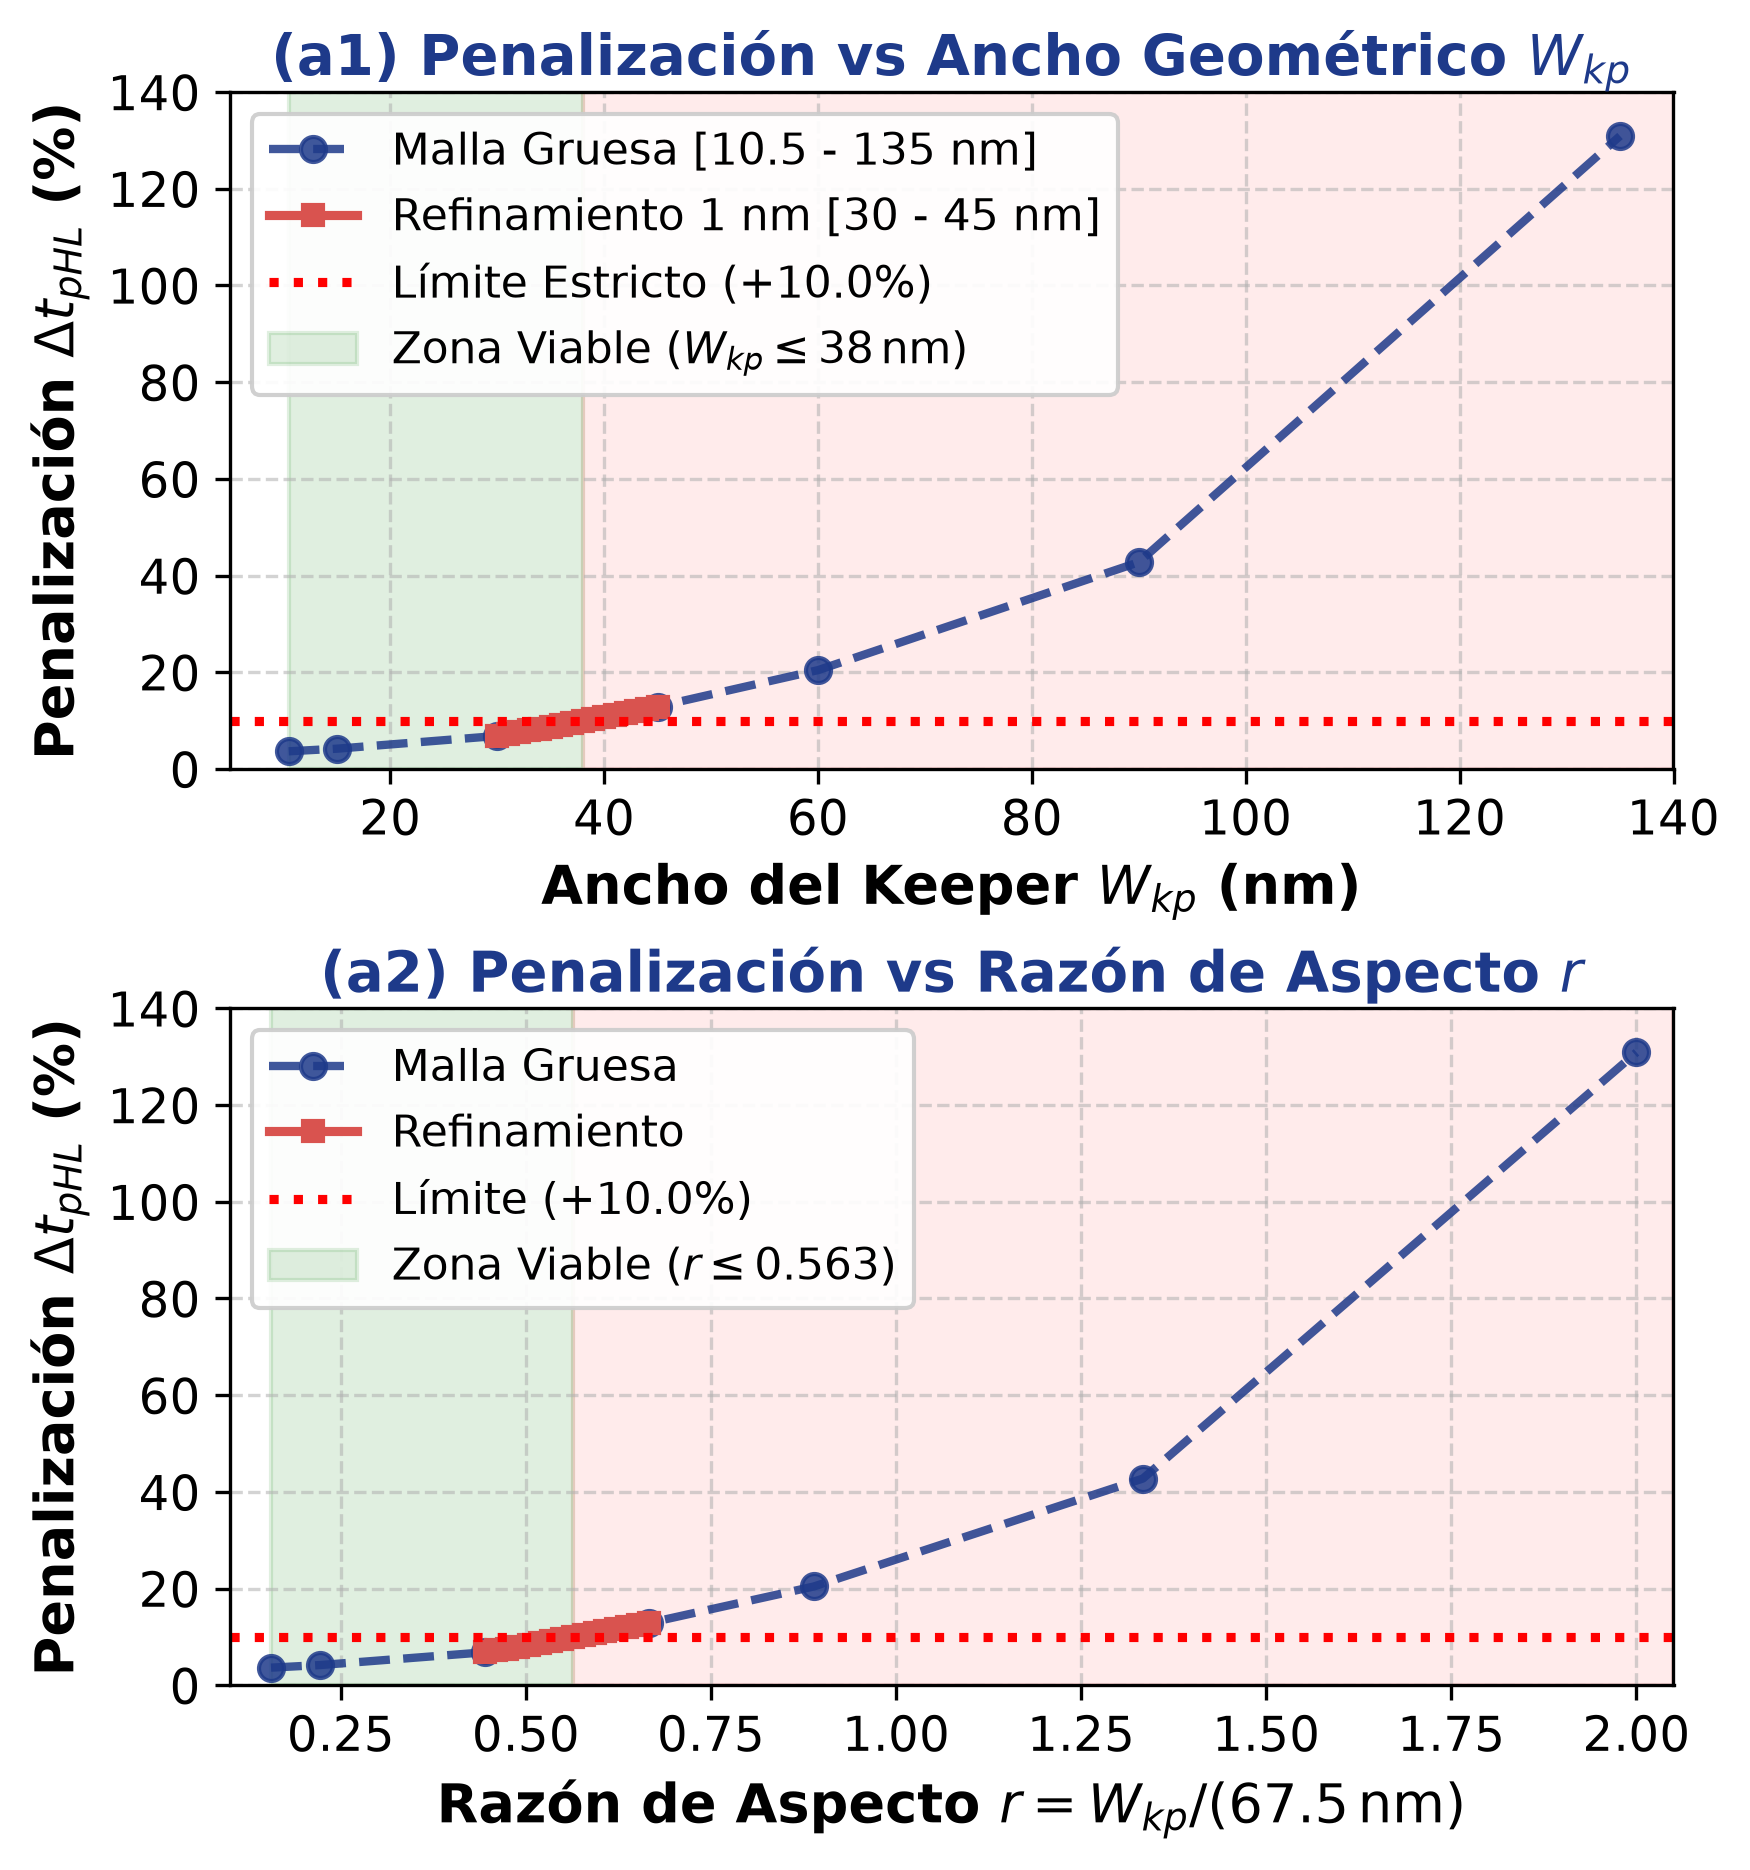
\includegraphics[width=0.68\linewidth]{figuras/fig3_act3_contencion_penalizacion.png}
  \caption[Penalización de retardo vs ancho del keeper y razón de aspecto]{Penalización porcentual del retardo de evaluación $\Delta t_{pHL}$ en función de $W_{kp}$ y de la razón de aspecto $r$ (45\,nm HP @ $85^\circ\text{C}$), identificando la malla gruesa y el refinamiento de 1\,nm en la frontera del 10.0\%.}
  \label{fig:contencion_penalizacion}
\end{figure}

Los resultados cuantitativos se exponen en la Tabla~\ref{tab:contencion} y en la Figura~\ref{fig:contencion_penalizacion}:
\begin{itemize}[leftmargin=1.4em,itemsep=0.15em]
  \item \textbf{Frontera Crítica en 45\,nm HP @ $85^\circ\text{C}$:} 
  \begin{itemize}[leftmargin=1.2em,itemsep=0.08em]
    \item $W_{kp} = 38.0\,\text{nm}$ ($r = 0.563$): es el \textbf{máximo ancho ensayado que satisface la cota de velocidad}, registrando $t_{pHL} = 34.96\,\text{ps}$ ($\Delta t_{pHL} = \mathbf{+9.94\%}$ bajo Configuración A y $\mathbf{+9.96\%}$ bajo Configuración B de alta precisión numérica).
    \item $W_{kp} = 39.0\,\text{nm}$ ($r = 0.578$): es el primer ancho ensayado que \textbf{incumple la cota}, alcanzando $\Delta t_{pHL} = \mathbf{+10.35\%}$.
    \item Un keeper convencional unitario ($W_{kp} = 45\,\text{nm}$, $r = 0.667$) induce una degradación inadmisible de $+12.90\%$ ($t_{pHL} = 35.90\,\text{ps}$), drenando una corriente de pico de contención de $I_{kp,\max} = 17.65\,\mu\text{A}$.
    \item Para anchos desmedidos ($W_{kp} = 180\,\text{nm}$, $r = 2.667$), la contención impide que la PDN descargue el nodo ($V_{dyn,\min} = 0.633\,\text{V} > V_M$), provocando una falla lógica catastrófica por pérdida total de conmutación.
  \end{itemize}
  \item \textbf{Frontera Crítica en 45\,nm LP @ $85^\circ\text{C}$:} Debido a la menor corriente de saturación de la PDN, el límite estricto se desplaza a $W_{kp} = 36.0\,\text{nm}$ ($r = 0.533$), el cual cumple con $\Delta t_{pHL} = \mathbf{+9.99\%}$ ($116.30\,\text{ps}$), mientras que $37.0\,\text{nm}$ supera el umbral con $\mathbf{+10.45\%}$.
\end{itemize}

\subsection{Compromiso Retención/Velocidad y Ventana de Viabilidad Conjunta}
La intersección simultánea de ambos requerimientos define la \textbf{ventana de viabilidad conjunta}:
\begin{equation}
  \mathcal{W}_{\text{viable}} = \left\{ W_{kp} \in \mathbb{R}^+ \;:\; V_{dyn}(1.0\,\mu\text{s}) \ge 0.90\,V_{DD} \quad \land \quad \Delta t_{pHL}(W_{kp}) < 10.0\% \right\}
\end{equation}

\begin{figure}[htbp]
  \centering
  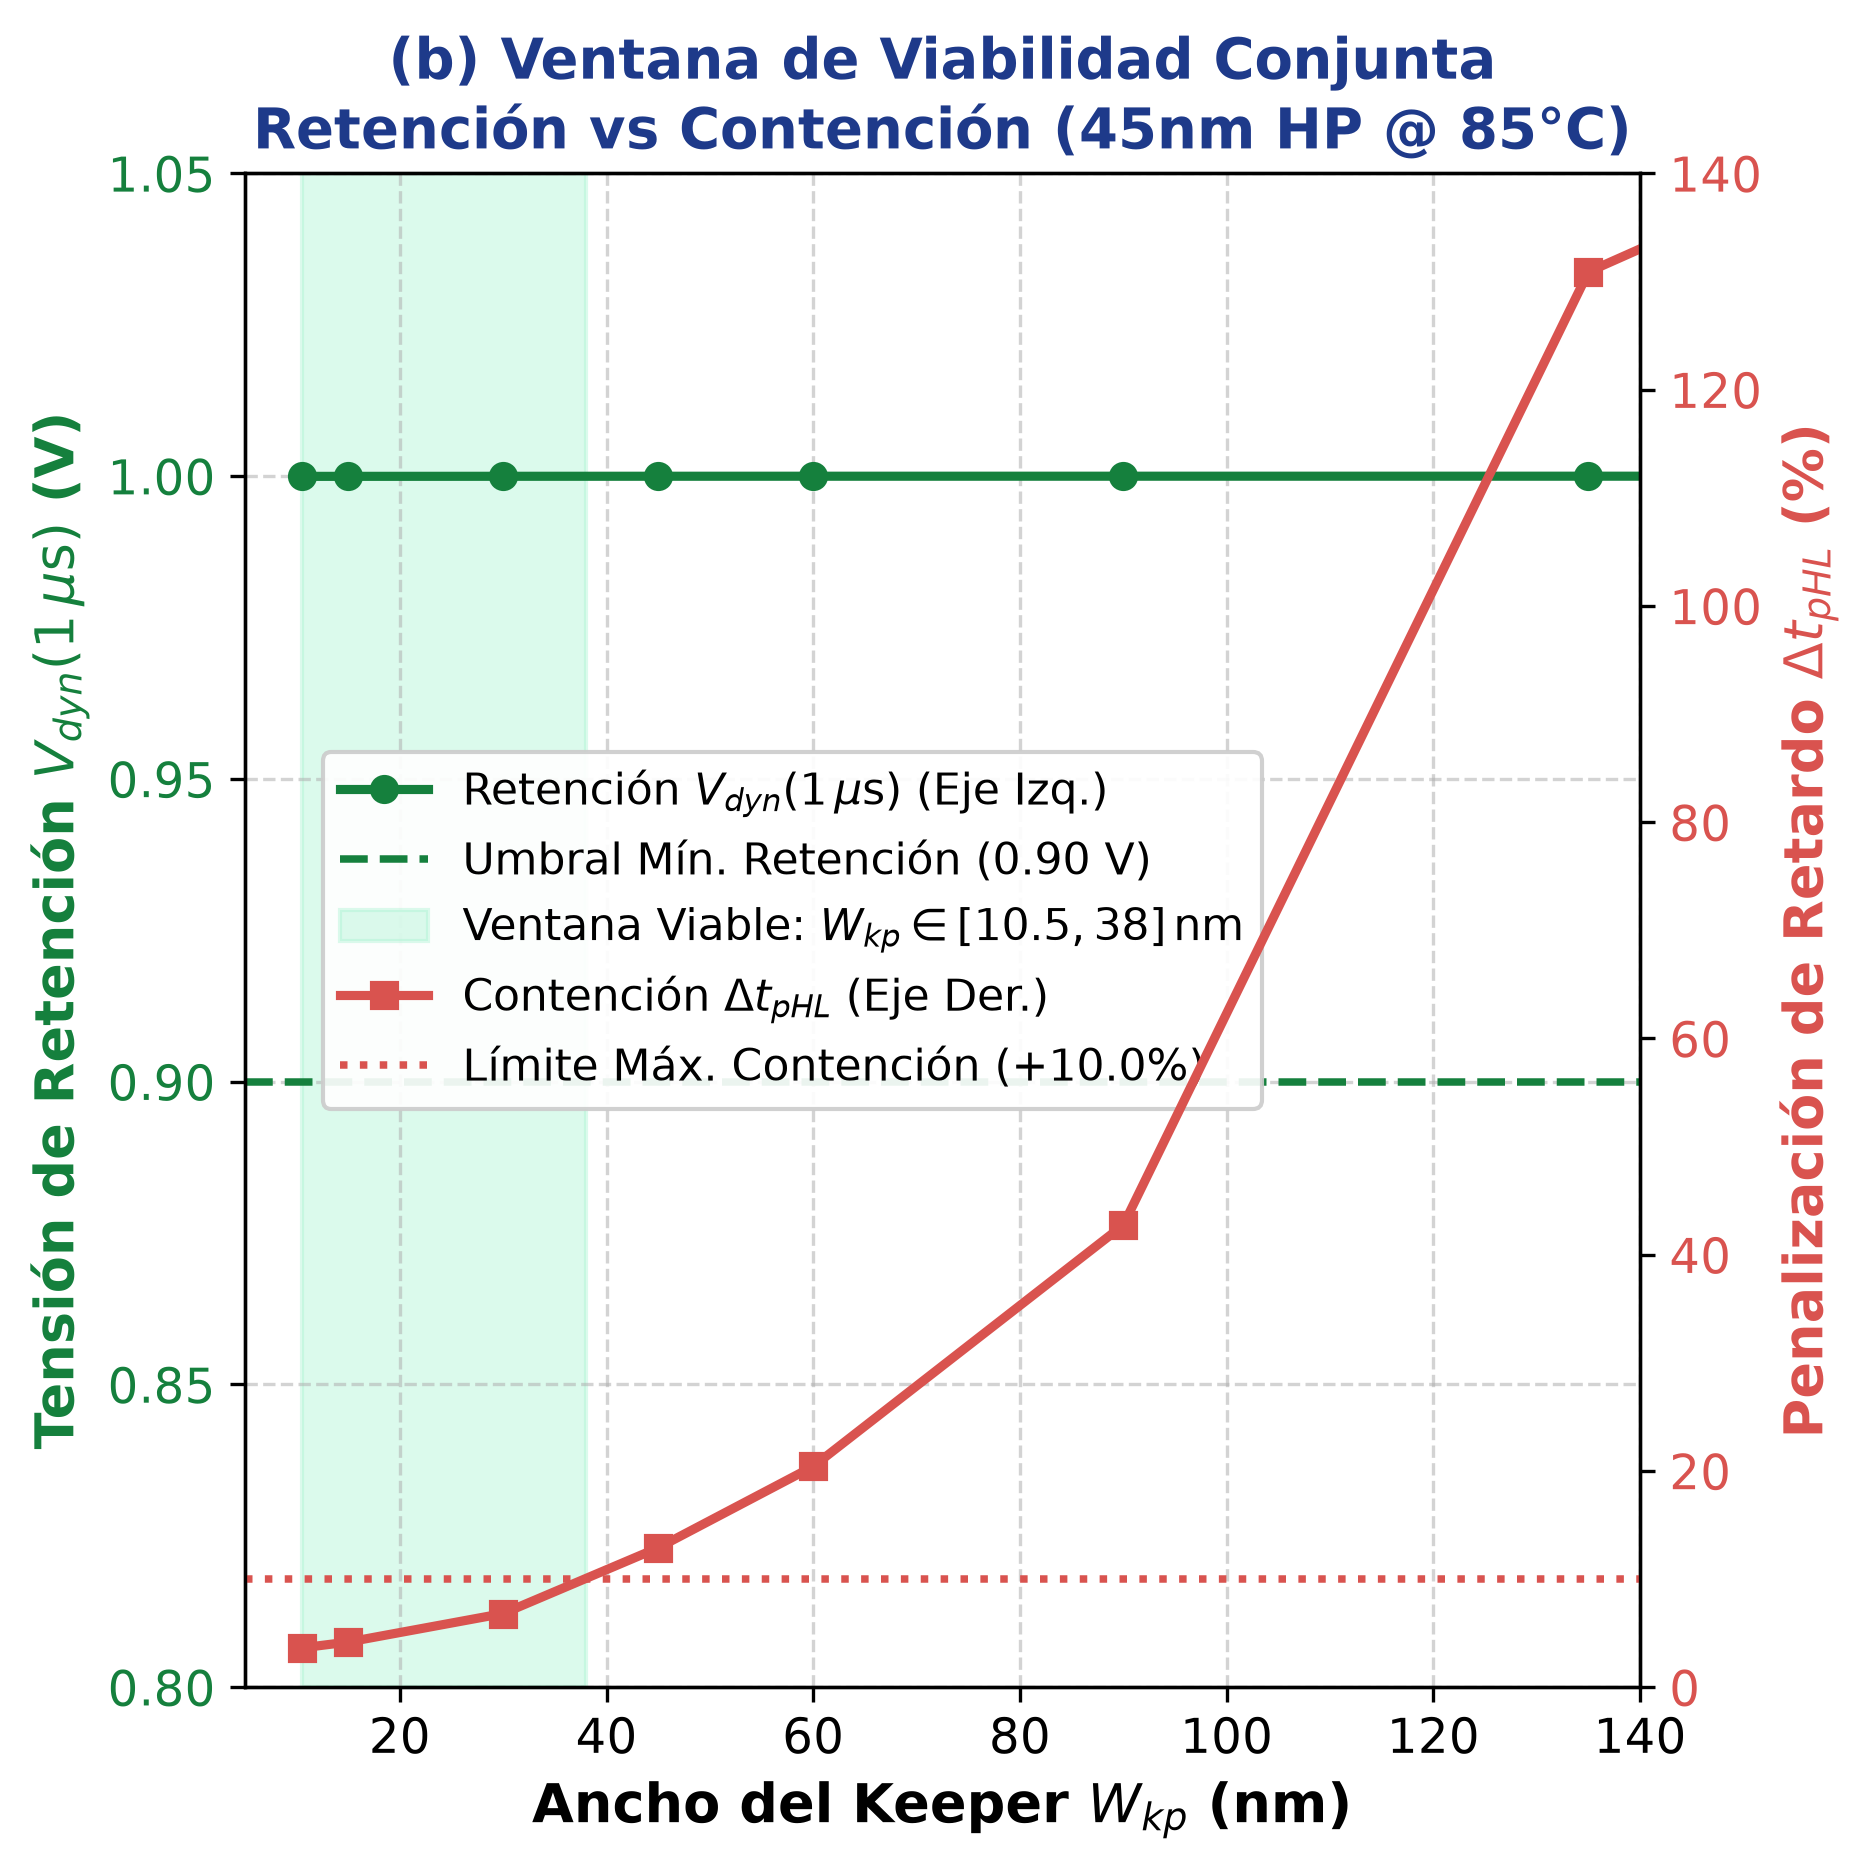
\includegraphics[width=0.62\linewidth]{figuras/fig4_act3_ventana_viabilidad.png}
  \caption[Ventana de viabilidad conjunta retención vs contención]{Ventana de viabilidad conjunta retención vs contención para la NAND3 en 45\,nm HP a $85^\circ\text{C}$. Los puntos de retención entre 31\,nm y 34\,nm se infieren a partir de la tendencia observada en los puntos simulados y la monotonicidad teórica esperada de la corriente del keeper con el ancho de canal, mientras que los valores de contención provienen de simulación transitoria directa.}
  \label{fig:ventana_viabilidad}
\end{figure}

Como se ilustra en la Figura~\ref{fig:ventana_viabilidad}, en 45\,nm HP a $85^\circ\text{C}$, la ventana viable delimitada sobre la malla de simulación comprende:
\begin{equation}
  W_{kp} \in [10.5\,\text{nm},\; 38.0\,\text{nm}] \quad \iff \quad r \in [0.156,\; 0.563]
\end{equation}
\noindent\textbf{Delimitación Metodológica de Evidencia Directa e Inferida:}
El respaldo experimental sobre la malla ensayada distingue tres regímenes: (1)~\textbf{Puntos viables con simulación directa completa}: los anchos $W_{kp} = 10.5$, $15$, $22$, $30$, $35$, $36$, $37$ y $38\,\text{nm}$ cuentan con simulaciones independientes de retención durante $1.0\,\mu\text{s}$ y de retardo activo, verificando simultáneamente ambos criterios con una penalización máxima de $\mathbf{+9.94\%}$ en $38\,\text{nm}$. (2)~\textbf{Punto de control externo de frontera}: $W_{kp} = 39\,\text{nm}$, ensayado directamente en ambos requisitos, queda fuera de la ventana viable al identificar el primer incumplimiento estricto de velocidad ($\Delta t_{pHL} = \mathbf{+10.35\%}$). (3)~\textbf{Retención inferida}: para los anchos intermedios $W_{kp} = 31$, $32$, $33$ y $34\,\text{nm}$, la contención proviene de simulación transitoria directa en malla de $1\,\text{nm}$, mientras que la retención durante $1\,\mu\text{s}$ se infiere por la monotonicidad teórica de la corriente restauradora y la cota observada en los extremos simulados ($V_{dyn} > 0.9999\,\text{V}$ en $30$ y $35\,\text{nm}$).

Por consiguiente, la ventana viable $[10.5,\, 38.0]\,\text{nm}$ queda demostrada empíricamente sobre la malla ensayada, sin postular continuidad analítica universal para todo valor intermedio ni reglas de diseño de fabricación (DRC) comerciales.

\subsection{Alternativas de Diseño: Keeper Condicional con Línea de Retardo}
La respuesta a la tarea~5 de la guía confirma que, aunque existe una ventana viable en 45\,nm HP, esta se encuentra restringida a anchos sub-micrométricos estrechos ($W_{kp} \le 38\,\text{nm}$). Un diseñador que restrinja el keeper al transistor unitario de referencia cuadrada ($W = L = 45\,\text{nm}$), adoptado como cota de dimensionamiento frente a anchos sub-litográficos sin respaldo de reglas DRC comerciales, queda automáticamente fuera de la especificación de velocidad ($\Delta t_{pHL} = +12.90\%$, con $t_{pHL} = 35.90\,\text{ps}$).

Para superar esta limitación, se implementó y ensayó la arquitectura de \textbf{Keeper Condicional} en el marco de este proyecto. La topología reemplaza el transistor simple por dos dispositivos PMOS en serie ($W = 45\,\text{nm}$ cada uno):
\begin{itemize}[leftmargin=1.4em,itemsep=0.12em]
  \item $M_{k,fb}$: Conectado al nodo dinámico $dyn$, gobernado por la salida $out$ como lazo de realimentación.
  \item $M_{k,en}$: Conectado a $V_{DD}$, gobernado por una señal de habilitación retrasada $CLK_{\text{del}}$ generada por una cadena de 3 inversores estáticos ($W_n = 90\,\text{nm}, W_p = 135\,\text{nm}$, retardo $\tau_{\text{del}} \approx 16.15\,\text{ps}$).
\end{itemize}

\begin{figure}[htbp]
  \centering
  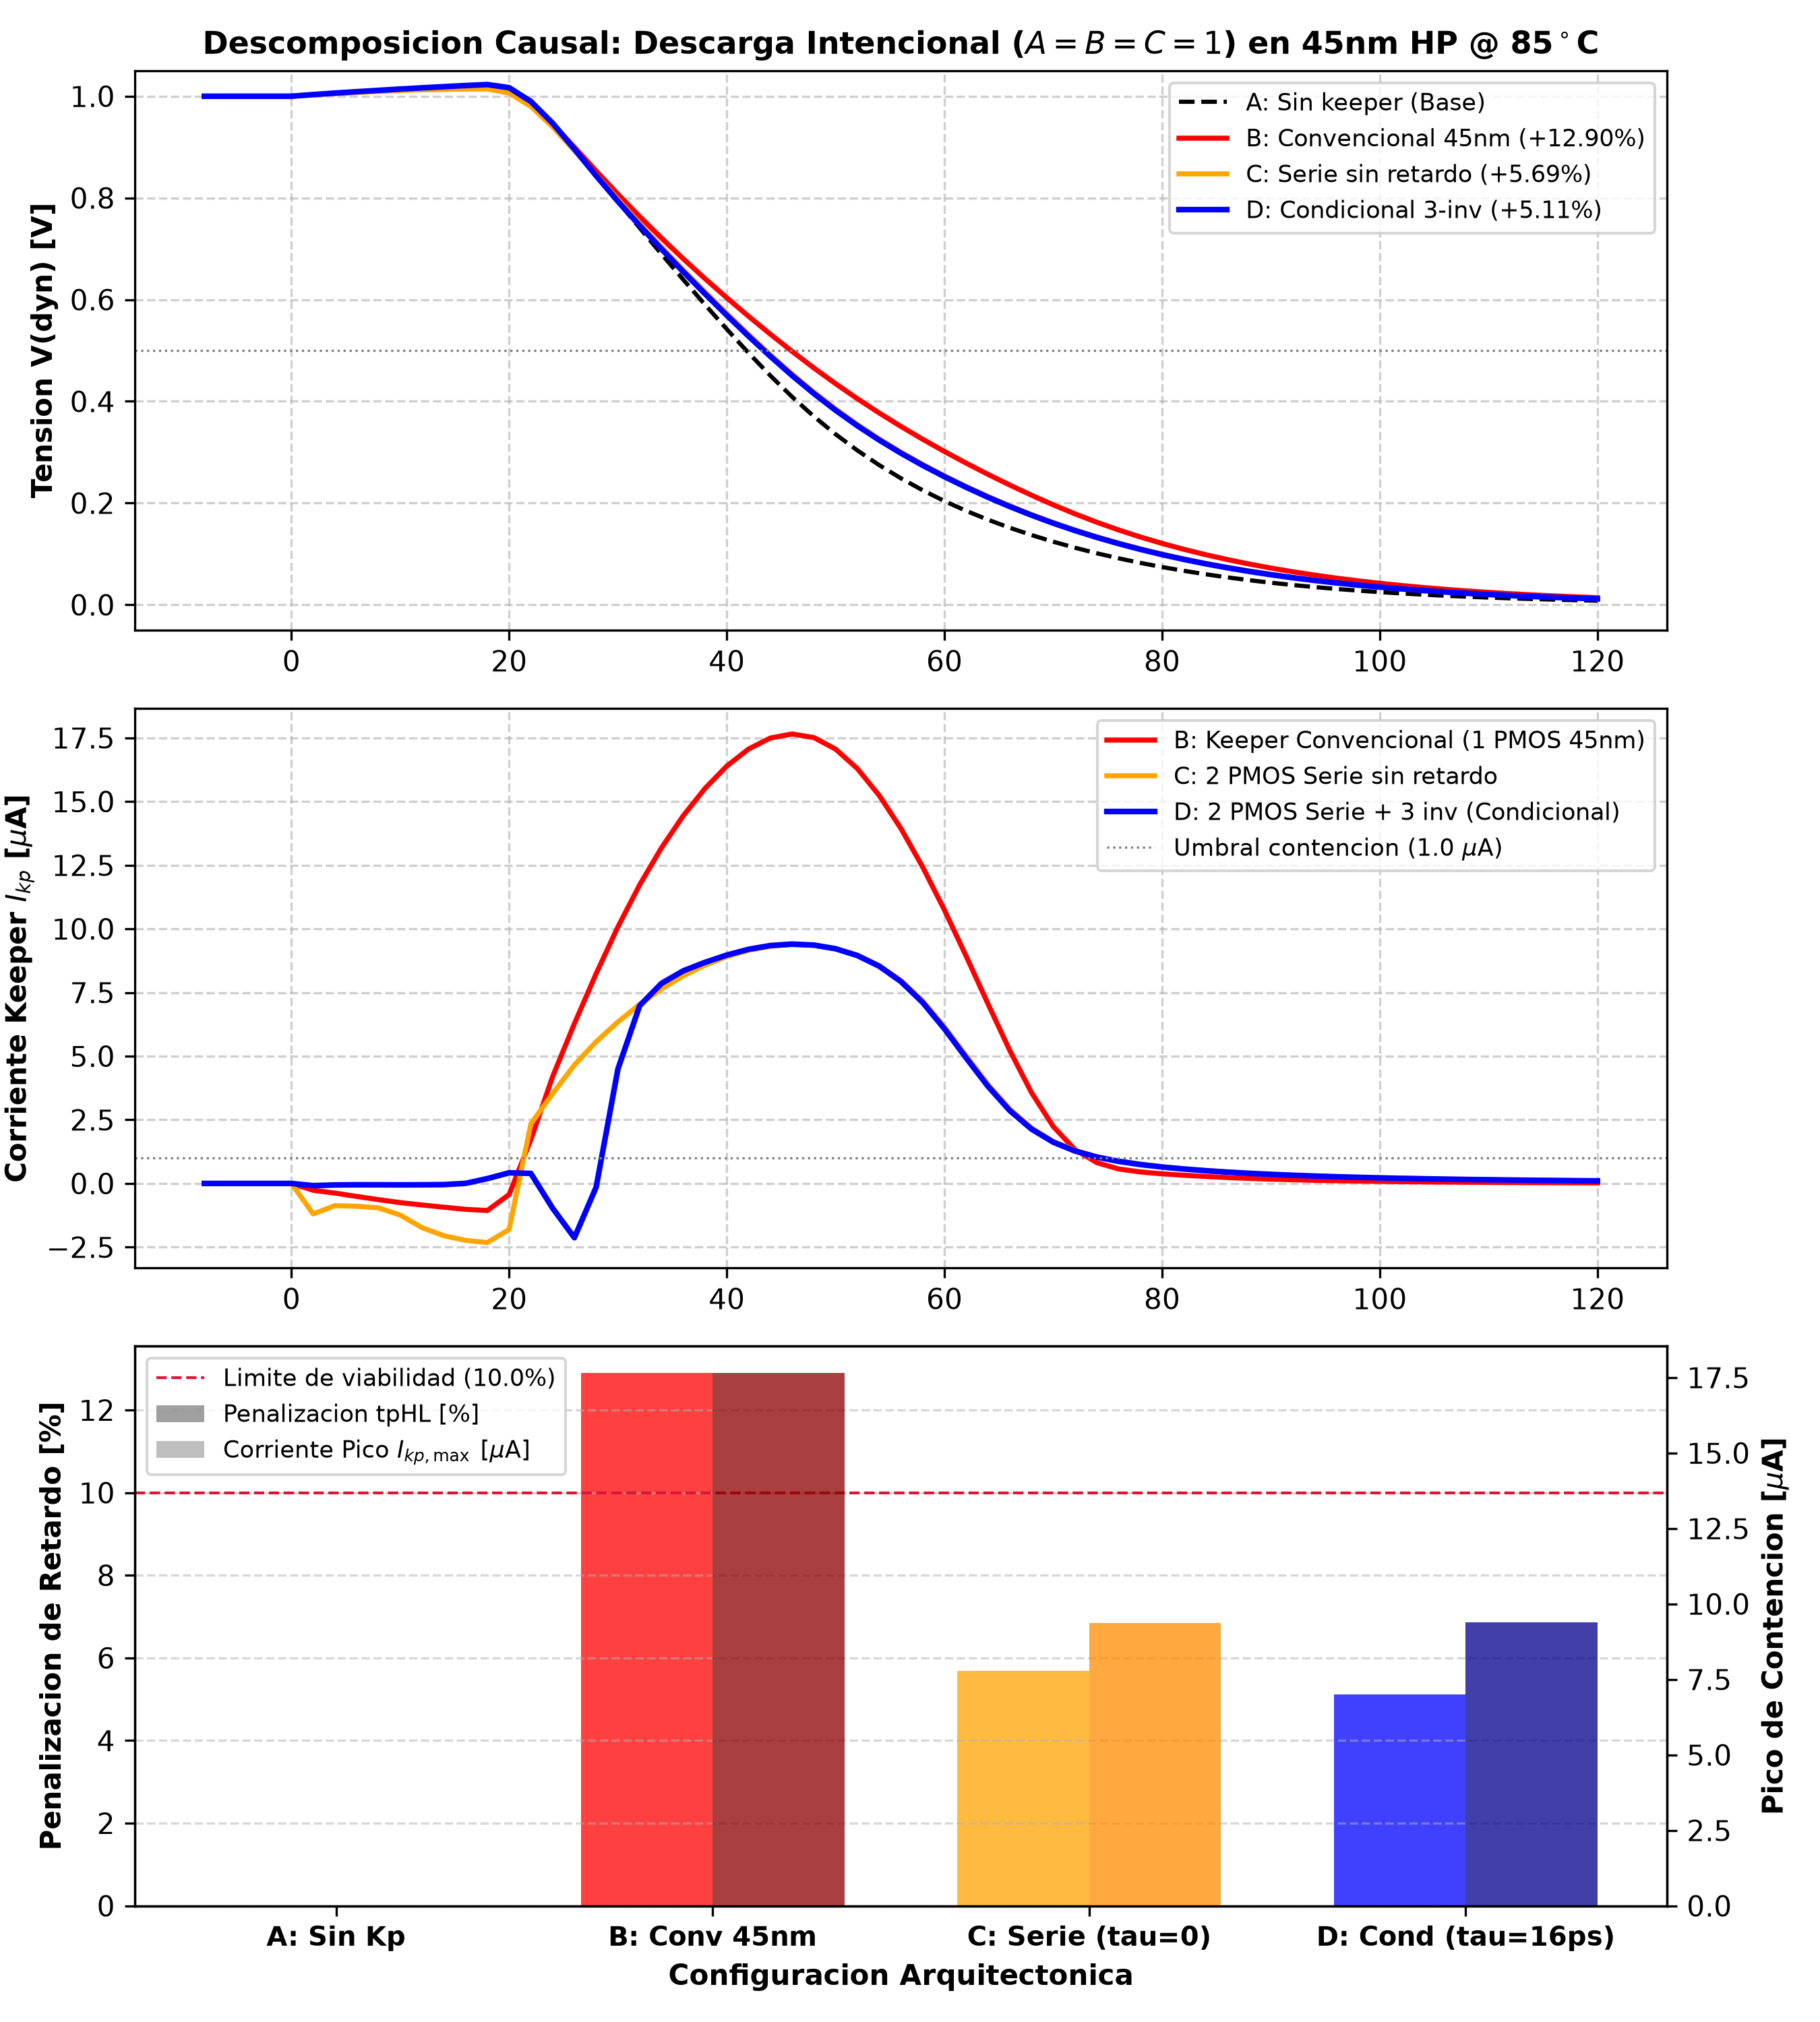
\includegraphics[width=0.62\linewidth]{figuras/fig5_act3_keeper_condicional.png}
  \caption[Descomposición causal del keeper condicional]{Descomposición causal del transitorio de evaluación activa ($A=B=C=1$) en 45\,nm HP a $85^\circ\text{C}$, comparando las formas de onda $V(dyn)$, la corriente instantánea de contención $I_{kp}(t)$ y la penalización de retardo.}
  \label{fig:keeper_condicional}
\end{figure}

La Figura~\ref{fig:keeper_condicional} detalla la respuesta transitoria y la corriente instantánea de contención, contrastando cuatro arquitecturas:
\begin{enumerate}[leftmargin=1.4em,itemsep=0.15em]
  \item \textbf{A (Sin Keeper):} Referencia base ideal sin contención ($t_{pHL} = 31.80\,\text{ps}$).
  \item \textbf{B (Keeper Convencional de 45\,nm):} Fuerte contención con pico $I_{kp,\max} = 17.65\,\mu\text{A}$, extendiéndose durante $50.0\,\text{ps}$ (intervalo de solapamiento $t \in [22.0,\, 72.0]\,\text{ps}$) y penalizando el retardo en $\mathbf{+12.90\%}$ ($35.90\,\text{ps}$).
  \item \textbf{C (Control de 2 PMOS Serie Síncronos, $\tau=0\,\text{ps}$):} Al disponer dos PMOS en serie comandados síncronamente, la duplicación de la resistencia de canal abate el pico de corriente a $9.38\,\mu\text{A}$ (reducción de 46.9\%), reduciendo la penalización a $\mathbf{+5.69\%}$ ($33.61\,\text{ps}$) con una duración de solapamiento de $52.0\,\text{ps}$ ($t \in [22.0,\, 74.0]\,\text{ps}$).
  \item \textbf{D (Keeper Condicional con 3 Inversores de Retardo):} La cadena retardada introduce un desfase en el inicio de la contención ($t_{\text{start}} = 22.0 \to 30.0\,\text{ps}$) y anticipa el corte del keeper respecto a la descarga de $dyn$, reduciendo la duración del solapamiento de contención a $44.0\,\text{ps}$ ($t \in [30.0,\, 74.0]\,\text{ps}$). La penalización cae a $\mathbf{+5.11\%}$ ($33.43\,\text{ps}$).
\end{enumerate}

\noindent\textbf{Causalidad Física No Lineal y Rol del Retardo:} Es imperativo destacar la explicación física subyacente: en la configuración con cadena de retardo se observa simultáneamente una menor \textbf{duración temporal} del solapamiento de contención (de $52.0\,\text{ps}$ en C a $44.0\,\text{ps}$ en D, frente a $50.0\,\text{ps}$ en B) y una menor penalización de retardo (+5.69\% $\to$ +5.11\%), sin que se reduzca el valor pico de corriente de contención ($I_{kp,\max}$ pasa de $9.38\,\mu\text{A}$ a $9.40\,\mu\text{A}$, con una variación menor al $0.3\%$ atribuible a acoplamientos parásitos de compuerta). Si bien la reducción del tiempo de conflicto disminuye el intervalo durante el cual el keeper disputa portadores contra la red de descenso, no debe atribuirse causalidad exclusiva a dicho recorte temporal sin un experimento de ablación que desacople completamente el retardo de la conmutación de los transistores y las cargas nodales internas.

\noindent\textbf{Compromiso de Sobrecarga de Reloj (\textit{Clock Overhead}):} La inclusión del primer inversor de retardo agrega la capacitancia de su compuerta ($W_n=90\,\text{nm}, W_p=135\,\text{nm} \implies C_g \approx 0.279\,\text{fF}$) a la red de distribución de reloj, la cual originalmente excitaba únicamente a $M_p$ y $M_f$ ($C_{clk,\text{base}} \approx 0.503\,\text{fF}$). Esto representa un incremento puramente geométrico de área de compuerta estimado en $\Delta C_{clk}/C_{clk,\text{base}} \approx \mathbf{+55.5\%}$.

\noindent\textbf{Validación de Inmunidad y Robustez:}
\begin{itemize}[leftmargin=1.4em,itemsep=0.1em]
  \item \textbf{Retención Estática ($1.0\,\mu\text{s}$):} En reposo ($CLK=1, A=B=C=0$), la salida del tercer inversor se fija en nivel bajo permanente, manteniendo habilitado el keeper condicional y garantizando $V_{dyn}(1\,\mu\text{s}) = 1.0000\,\text{V}$ sin caída.
  \item \textbf{Recuperación frente a Compartición de Carga ($CLK=1, A=B=1, C=0$):} Sometido al peor caso de compartición (Actividad~2), el nodo experimenta una caída inicial a $V_{dyn,\min} = 0.9247\,\text{V}$ ($\Delta V = 75.3\,\text{mV}$); el keeper condicional restaura el potencial dinámico hasta $0.9980\,\text{V}$ antes de culminar la evaluación, asegurando que la salida se mantenga inmutable ($V_{out} < 0.18\,\text{mV}$).
\end{itemize}

En las condiciones y tiempos ensayados, el keeper condicional permite usar transistores de $45\,\text{nm}$ y cumplir simultáneamente la retención durante la ventana ensayada de $1\,\mu\text{s}$ y el límite de penalización de velocidad del 10\%. No se postula retención ilimitada; su comportamiento a escalas temporales mayores requeriría modelamiento adicional de fugas en reposo prolongado.

% ==============================================================================
% SECCION 5: ACTIVIDAD 4 - REGLA DE MONOTONICIDAD, CASCADA DOMINO Y SKEW DE RELOJ
% ==============================================================================
\needspace{3\baselineskip}
\section{Actividad 4: Regla de Monotonicidad, Cascada Dominó y Skew de Reloj}
\label{sec:actividad4}

En la lógica CMOS dinámica, la salida solo puede realizar una transición descendente ($1 \to 0$) durante la fase de evaluación. Cuando múltiples compuertas dinámicas se interconectan directamente en cascada, el estado inicial pre-cargado ($1$ lógico) de la primera etapa puede activar transitoriamente la red de conmutación (PDN) de la etapa posterior antes de que la evaluación se complete, induciendo pérdidas de carga irreversibles. Esta sección analiza experimentalmente la violación de la regla de monotonicidad, valida su mitigación mediante la estructura dominó clásica (con inversor estático intermedio), examina la vulnerabilidad ante entradas no monótonas y contrasta el compromiso temporal y energético entre cascadas \textit{Footed} y \textit{Unfooted} frente al \textit{skew} de reloj.

\subsection{Violación de Monotonicidad y Prevención de Activación Prematura}
Se simuló una cascada de dos etapas dinámicas NAND2 idénticas ($W_n = 90\,\text{nm}, W_p = 135\,\text{nm}, W_{\text{PDN}} = 180\,\text{nm}$, $C_L = 2.0\,\text{fF}$) a $500\,\text{MHz}$ ($T_{clk} = 2.0\,\text{ns}$) bajo PTM 45\,nm HP. Se contrastaron tres regímenes operativos, documentados en la Figura~\ref{fig:monotonicidad_cascada}:

\begin{enumerate}[leftmargin=1.4em,itemsep=0.01em]
  \item \textbf{Régimen A (Cascada Directa Sin Inversor, $A=B=X=1$):} El nodo $dyn1$ conecta directo a la compuerta receptora. Al pasar a evaluación ($CLK: 0 \to 1$), $dyn1$ drena con retardo finito $t_{pHL1}$. Como $X=1$, la segunda etapa conduce a masa y vacía espuriamente a $dyn2$ hasta $V_{dyn2,\min} = \mathbf{0.64624\,\text{V}} \implies \Delta V_{dyn2} = \mathbf{353.76\,\text{mV}}$, erosionando el margen de ruido ($NM_H = 67.7\,\text{mV}$, pérdida del $84\%$), aunque sin bascular de inmediato ($V_{dyn2} > V_M \approx 0.48\,\text{V}$).
  \item \textbf{Régimen B (Cascada Dominó con Inversor, $A=B=X=1$):} Con inversor intermedio ($W_n = 90\,\text{nm}, W_p = 135\,\text{nm}$), $out1=0\,\text{V}$ en precarga. En evaluación, $out1$ ejecuta una transición \textbf{monótona creciente ($0 \to 1$)} solo tras evaluar la primera etapa, descargando legítimamente $dyn2$ a $\mathbf{-0.00584\,\text{V}} \approx 0\,\text{V}$ y evaluando la función lógica global ($out2 \approx 1.0\,\text{V}$).
  \item \textbf{Régimen C (Control de Bloqueo con Inversor, $A=B=1, X=0$):} Con $X=0$, la PDN2 permanece bloqueada pese a que $out1=1\,\text{V}$, reteniendo íntegramente $V_{dyn2,\min} = \mathbf{0.999999\,\text{V}}$ ($\Delta V \approx \mathbf{0.000\,\text{mV}}$, $out2 = 26.8\,\text{nV}$), confirmando el bloqueo funcional.
\end{enumerate}

\begin{figure}[htbp]
  \centering
  \begin{minipage}[t]{0.485\textwidth}
    \centering
    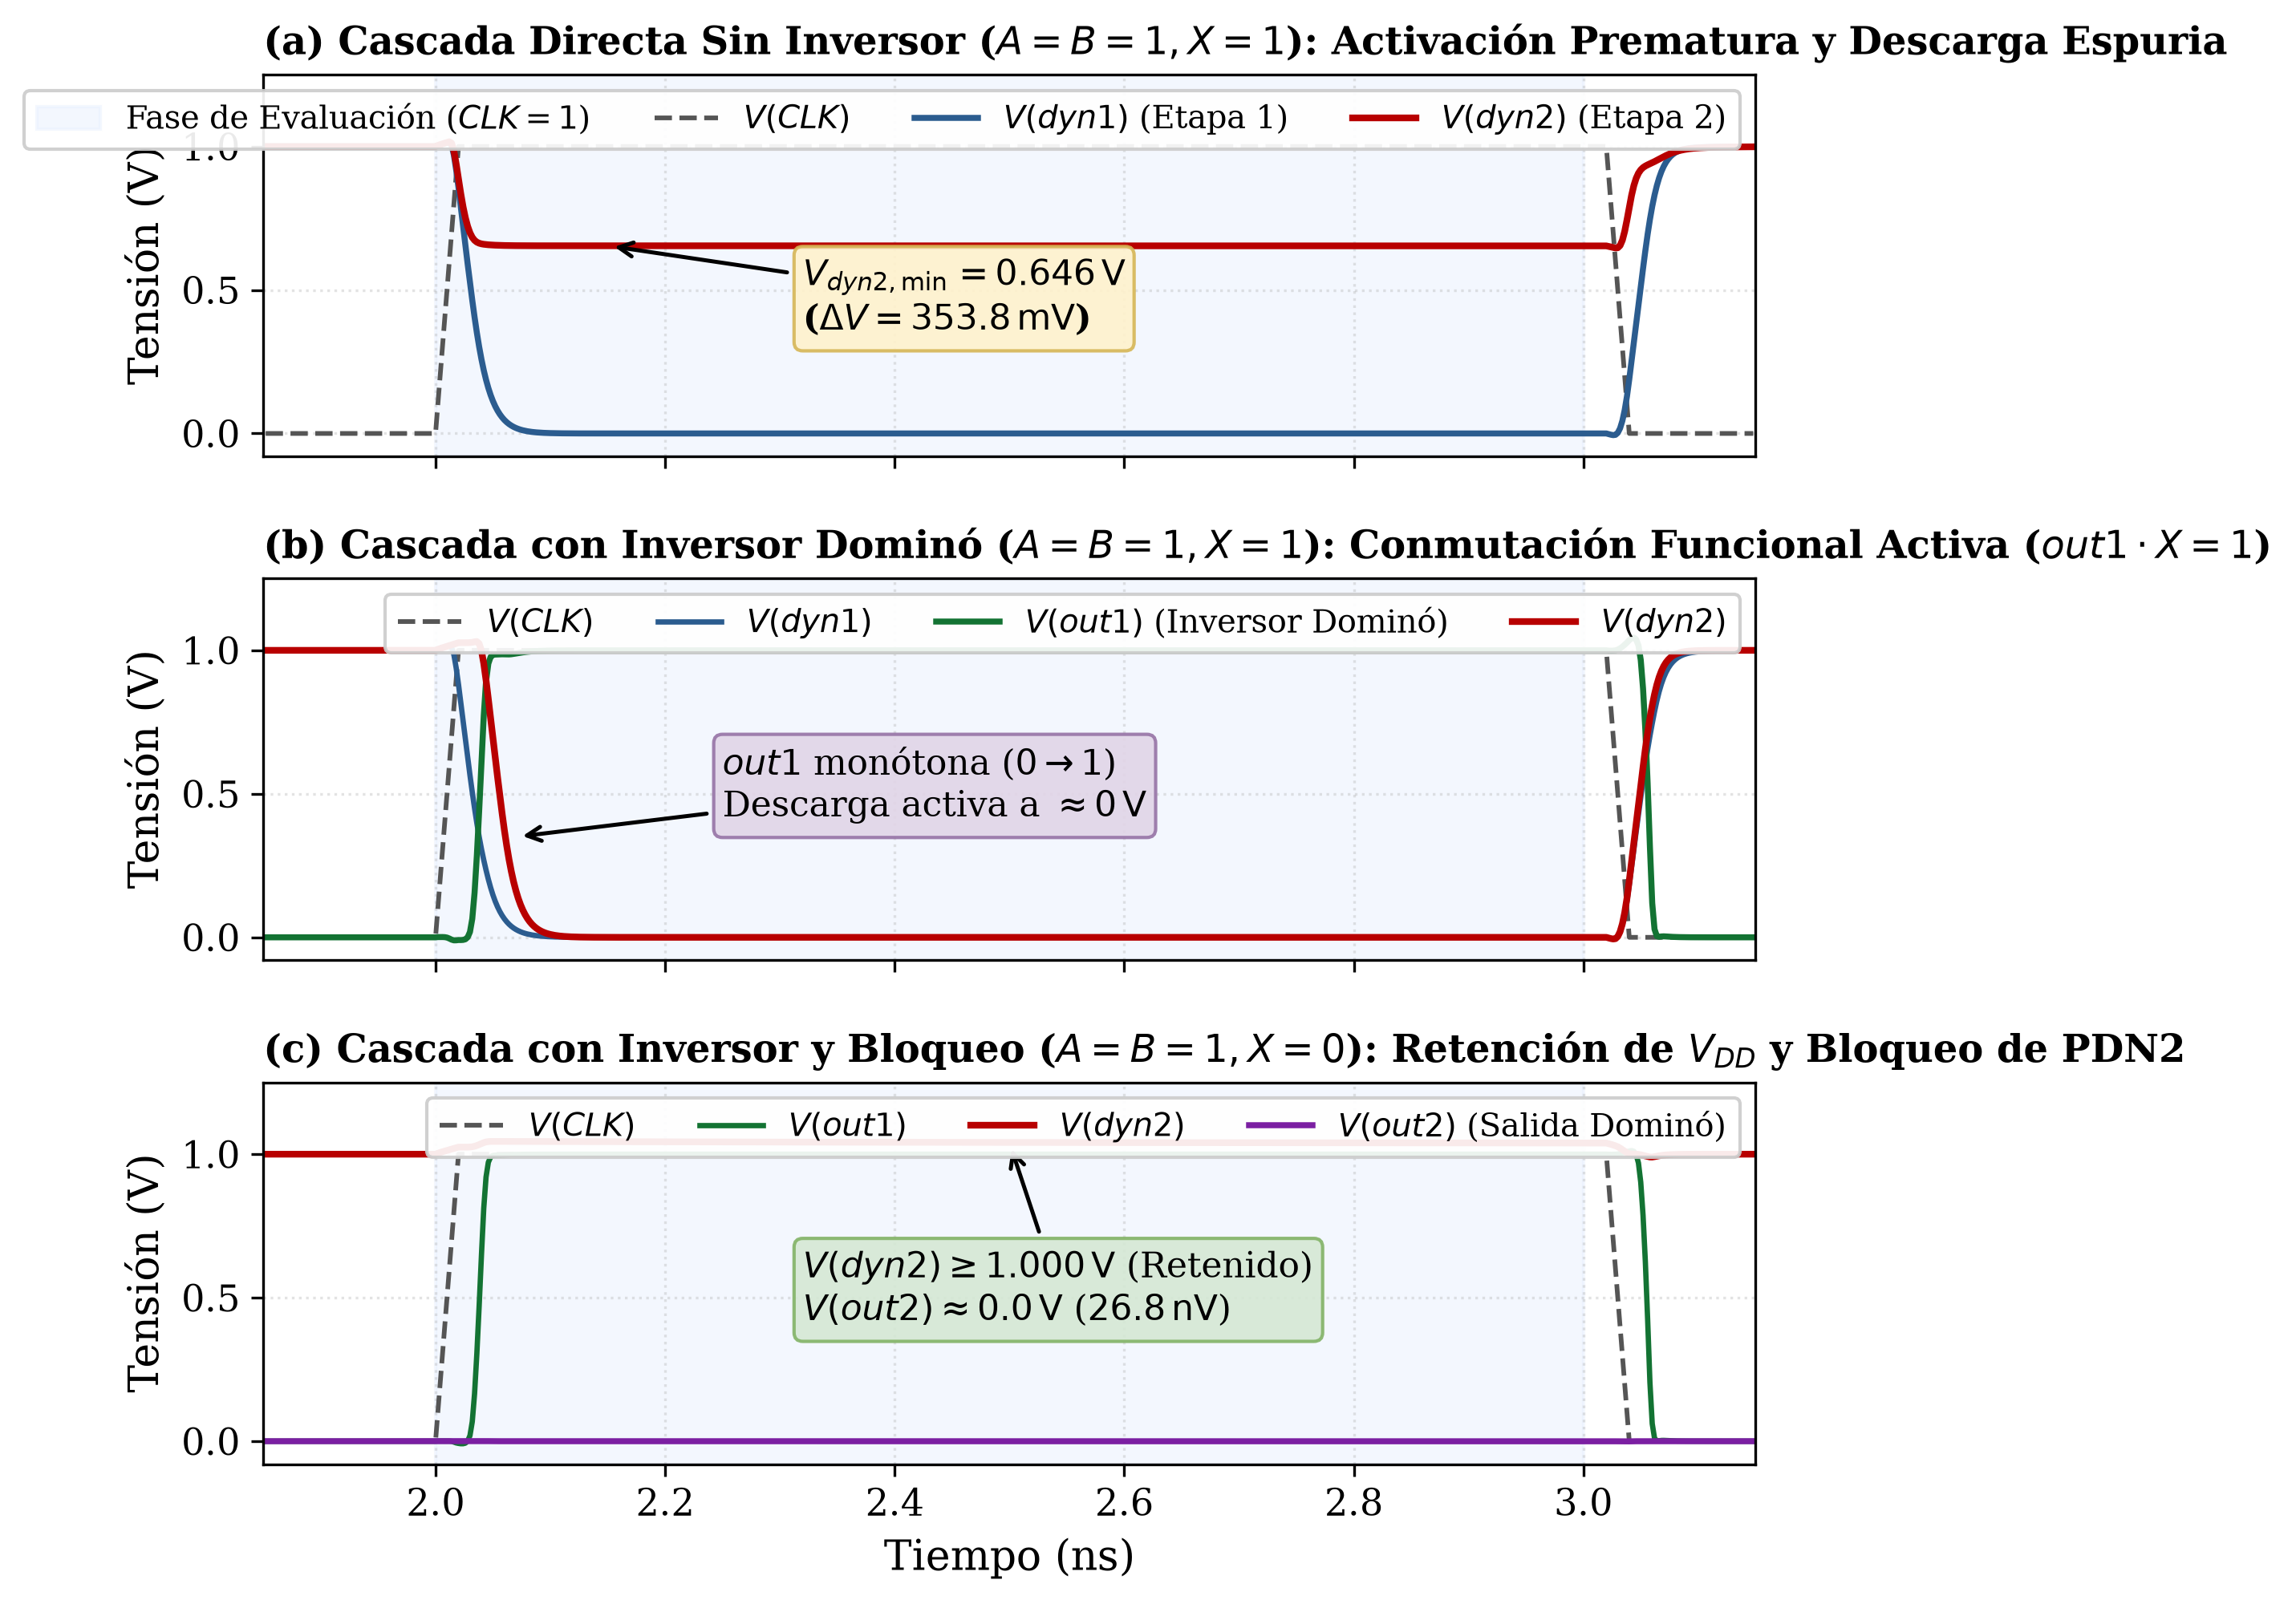
\includegraphics[width=\linewidth,height=4.3cm,keepaspectratio]{figuras/fig1_act4_monotonicidad_cascada.png}
    \caption[Análisis de regímenes de operación en cascada dominó]{Regímenes en cascada de 2 etapas NAND2 (45\,nm HP): (a) Directa sin inversor ($\Delta V = 353.8\,\text{mV}$); (b) Dominó ($dyn2 \approx 0\,\text{V}$); (c) Dominó con bloqueo ($X=0$, retención plena).}
    \label{fig:monotonicidad_cascada}
  \end{minipage}\hfill
  \begin{minipage}[t]{0.485\textwidth}
    \centering
    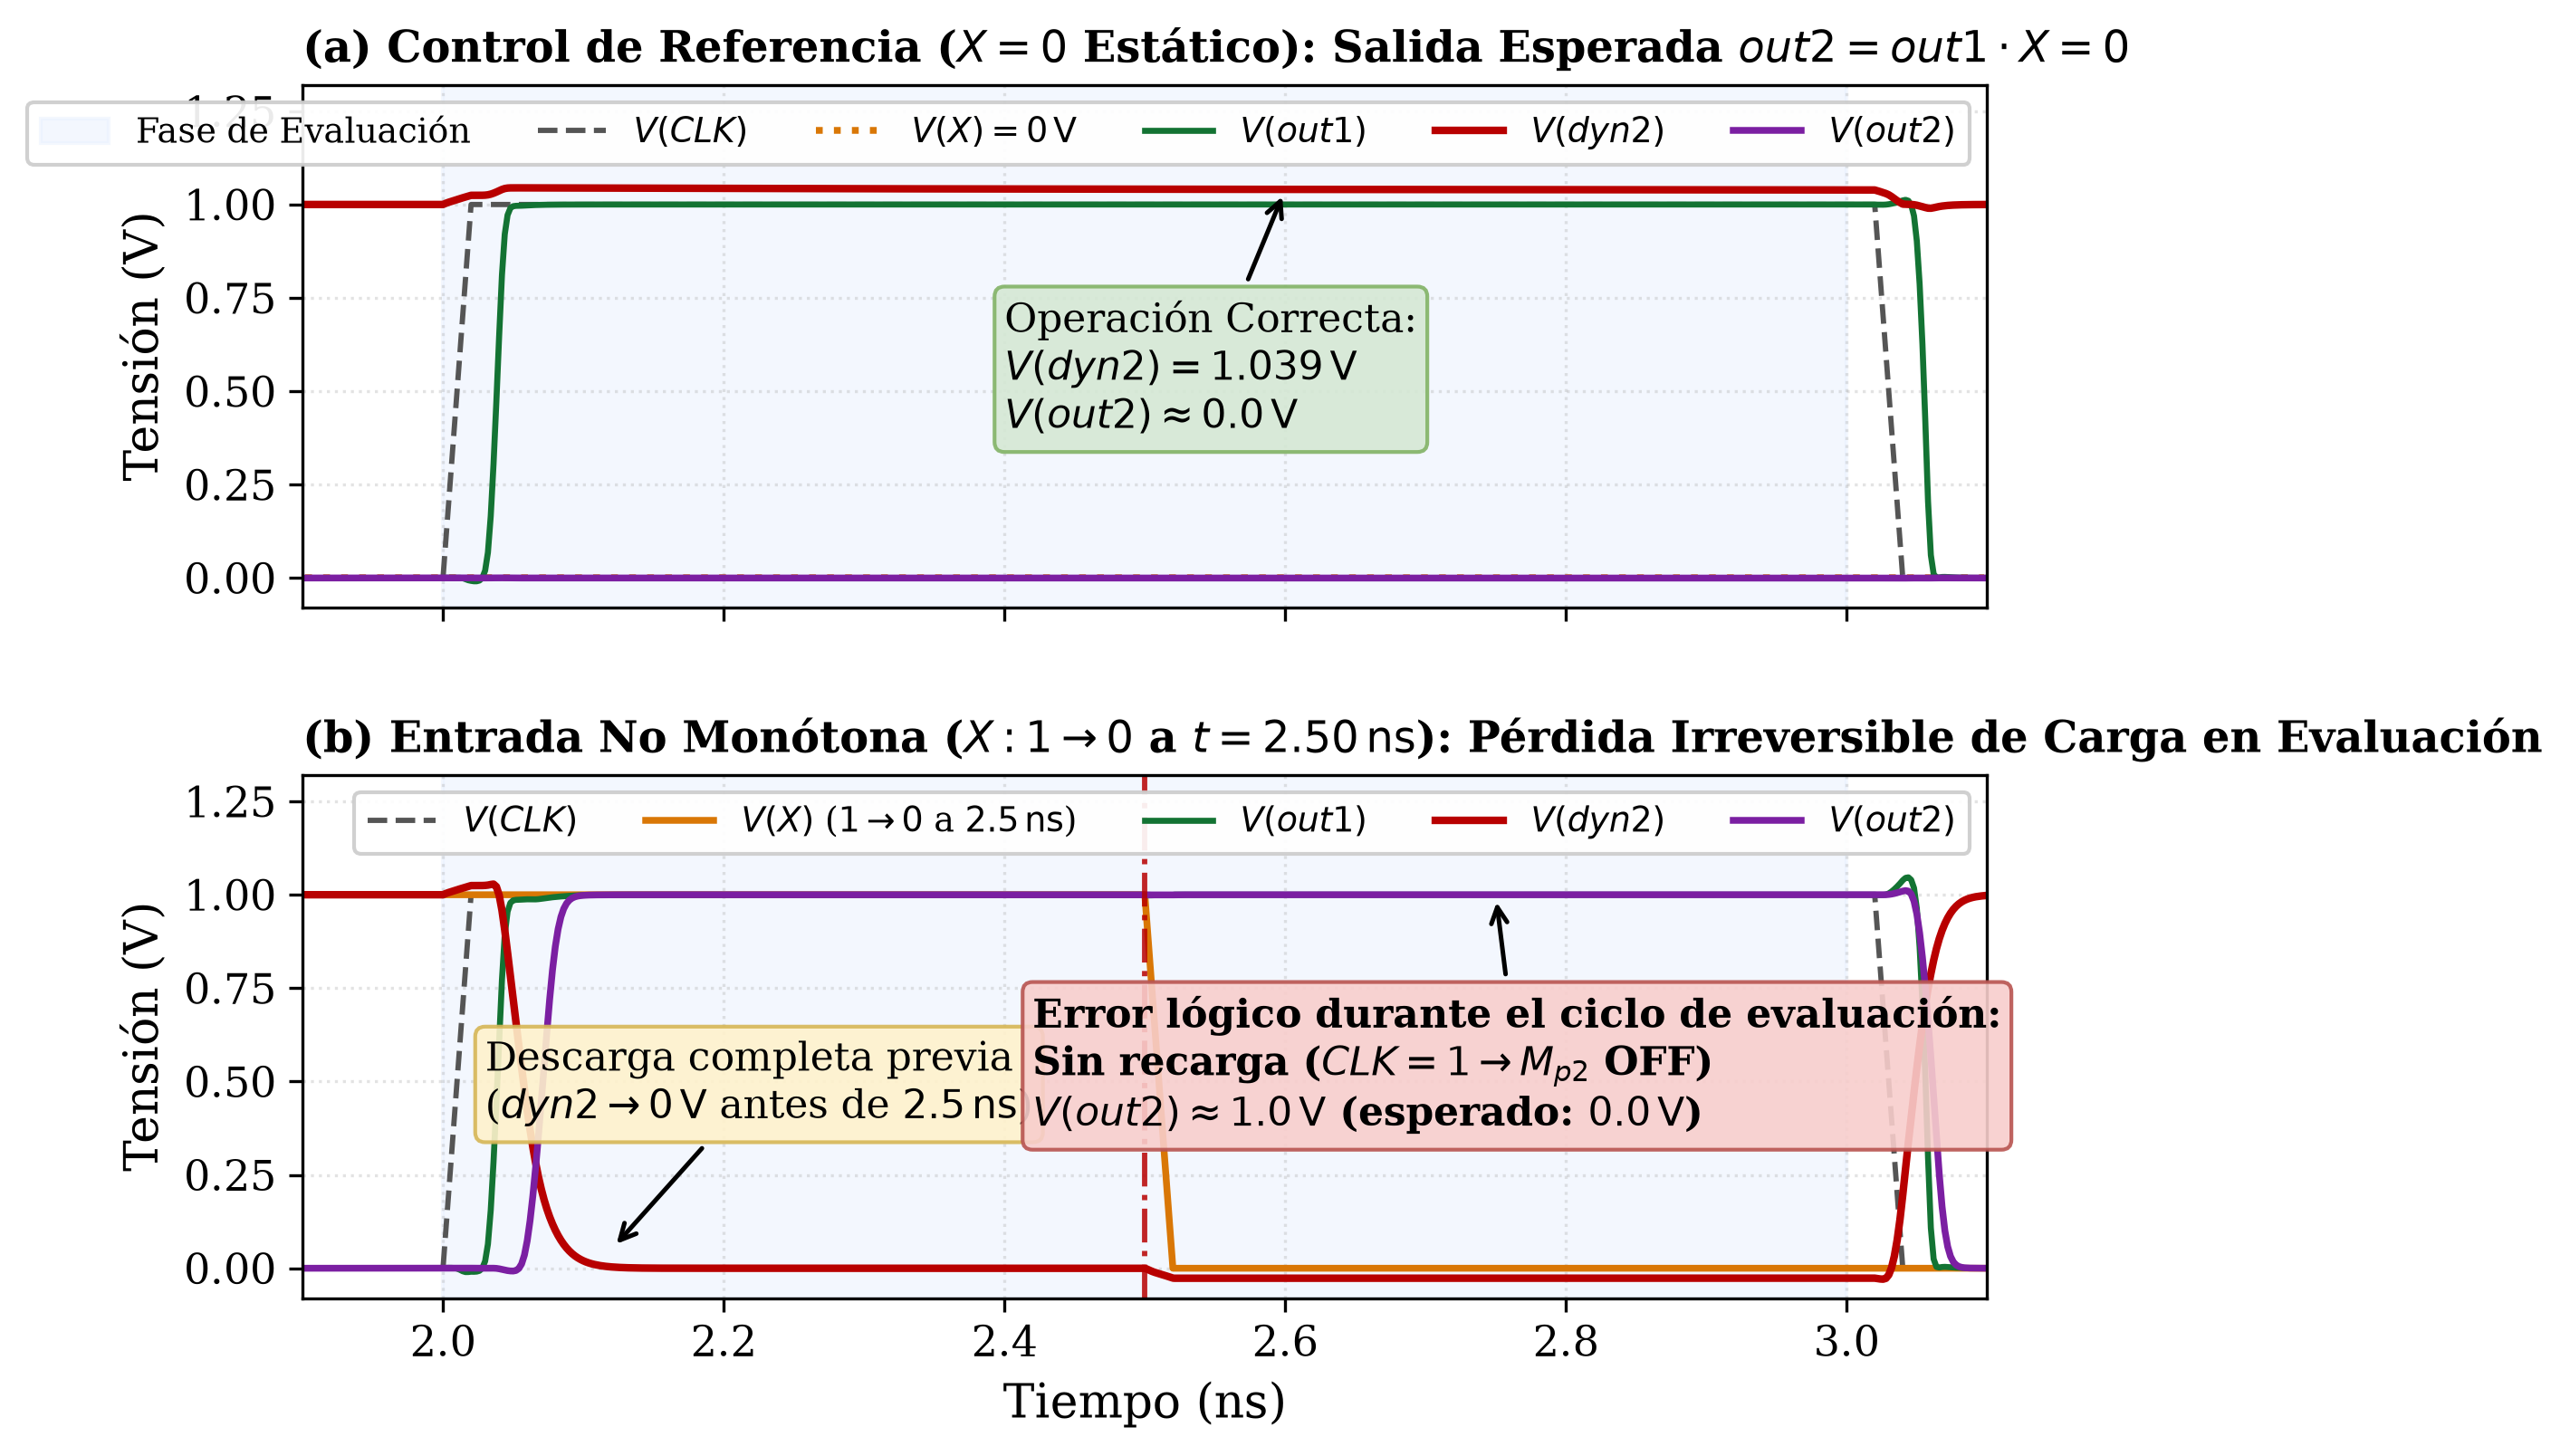
\includegraphics[width=\linewidth,height=4.3cm,keepaspectratio]{figuras/fig2_act4_pulso_x_descendente.png}
    \caption[Impacto de entrada externa no monótona]{Entrada externa no monótona (45\,nm HP): (a) Control $X=0$ estático ($out2 \approx 0\,\text{V}$); (b) Pulso descendente $X: 1 \to 0$ a $t=2.50\,\text{ns}$, evidenciando error lógico en ciclo activo.}
    \label{fig:pulso_x_descendente}
  \end{minipage}
\end{figure}

\subsection{Sensibilidad a Entradas Externas No Monótonas y Conexión con Flip-Flops}
Para evaluar la vulnerabilidad del nodo dinámico ante violaciones de la regla de monotonicidad en entradas externas, se modeló una compuerta dominó gobernada por $out1 \to 1$ donde la entrada externa $X$ experimenta una transición descendente ($1 \to 0$) a mitad de la fase de evaluación ($t = 2.50\,\text{ns}$). Los resultados se comparan con la referencia estática $X=0$:

\begin{itemize}[leftmargin=1.4em,itemsep=0.01em]
  \item \textbf{Descarga Previa a la Transición:} Entre $t=2.00\,\text{ns}$ y $t=2.50\,\text{ns}$, $X=1$ y $out1=1$. La PDN2 conduce y descarga $dyn2$ a tierra en $60\,\text{ps}$ ($V_{dyn2} = 3.66\,\mu\text{V}$ en $t=2.49\,\text{ns}$).
  \item \textbf{Interrupción sin Restauración:} A $t=2.50\,\text{ns}$, $X$ cae a $0\,\text{V}$ y apaga el NMOS inferior. Al estar el reloj en evaluación ($CLK=1$), el PMOS de precarga sigue cortado; al carecer de camino a $V_{DD}$, la carga \textbf{no se recupera en ese ciclo}.
  \item \textbf{Error Lógico en el Ciclo de Evaluación:} Al final de la fase ($t=2.99\,\text{ns}$), la lógica ideal exige $out2 = out1 \cdot X = 0$. Mientras el control estático entrega $out2 = 26.8\,\text{nV} \approx 0\,\text{V}$, con pulso se sostiene $dyn2 = -0.0265\,\text{V}$ y $out2 = \mathbf{0.999997\,\text{V}} \approx 1.0\,\text{V}$, constituyendo un \textbf{error lógico funcional por vaciado irreversible}.
  \item \textbf{Implicancia para Biestables (TGFF):} Las señales excitadoras desde biestables deben asegurar transiciones monótonas crecientes o niveles estables sin \textit{glitches} durante la evaluación para evitar la corrupción de datos.
\end{itemize}

\subsection{Cascada Dominó de Tres Etapas: Footed vs Unfooted y Skew de Reloj}
Para cuantificar el impacto del desalineamiento de reloj en cascadas de mayor profundidad lógica, se evaluó una estructura dominó NAND2 de 3 etapas en versiones \textit{Footed} (con $M_f$) y \textit{Unfooted} (sin $M_f$) bajo un barrido de skew temporal ($T_{\text{skew}} \in [-50, 200]\,\text{ps}$). La Tabla~\ref{tab:skew_act4} y la Figura~\ref{fig:footed_vs_unfooted_skew} consolidan las mediciones.

% Tabla de caracterizacion de cascada domino de 3 etapas Footed vs Unfooted bajo barrido de skew de reloj
% Fuente primaria: Tarea 4 Footed.log y Paso 5 Unfooted.log (PTM 45nm HP, VDD = 1.0 V, T = 27 C)
\begin{table}[htbp]
\centering
\fontsize{7.5pt}{8.8pt}\selectfont
\caption[Caracterización de cascada dominó de 3 etapas Footed vs Unfooted]{Respuesta temporal y picos de corriente de alimentación en cascada dominó de 3 etapas (NAND2) bajo barrido de skew de reloj ($T_{\text{skew}} \in [-50, 200]\,\text{ps}$): contraste entre arquitecturas Footed y Unfooted.}
\label{tab:skew_act4}
\begin{tabularx}{\linewidth}{@{}>{\centering\arraybackslash}p{1.2cm} c c c c c c >{\RaggedRight\arraybackslash}X@{}}
\toprule
\textbf{$T_{\text{skew}}$} & \textbf{$t_{\text{del}}$ (Foot)} & \textbf{$t_{\text{del}}$ (Unfoot)} & \textbf{$\Delta t_{\text{del}}$} & \textbf{$I_{\text{pk}}$ (Foot)} & \textbf{$I_{\text{pk}}$ (Unfoot)} & \textbf{$\Delta I_{\text{pk}}$} & \textbf{Diagnóstico Físico / Condición de Operación} \\
\textbf{(ps)} & \textbf{(ps)} & \textbf{(ps)} & \textbf{(\%)} & \textbf{($\mu\text{A}$)} & \textbf{($\mu\text{A}$)} & \textbf{($\mu\text{A}$)} & \textbf{(Ventana de medición: $t \in [0.5, 4.5]\,\text{ns}$)} \\
\midrule
$-50$ & 77.20 & 66.46 & $-13.9\%$ & 113.80 & 326.30 & $+212.50$ & Precarga adelantada en etapas 2 y 3 drena a través de la PDN en conducción. \\
$0$   & 77.21 & 66.47 & $-13.9\%$ & 318.85 & 332.91 & $+14.06$  & Sincronismo pleno: las 3 etapas precargan simultáneamente en paralelo. \\
$+50$ & 125.47 & 95.12 & $-24.2\%$ & 110.56 & 110.57 & $+0.01$   & Desacoplo de precargas; corriente limitada al pico capacitivo de una etapa. \\
$+100$& 226.68 & 130.81& $-42.3\%$ & 110.56 & 160.57 & $+50.01$  & Incremento de corriente en unfooted por conducción simultánea PMOS/PDN. \\
$+200$& 426.91 & 171.48& $-59.8\%$ & 110.56 & 214.63 & $+104.07$ & Elevación de pico de alimentación ($+94.1\%$); Footed inmune a corto. \\
\bottomrule
\end{tabularx}
\end{table}


\begin{itemize}[leftmargin=1.4em,itemsep=0.0em]
  \item \textbf{Ahorro a Skew Nulo ($T_{\text{skew}}=0\,\text{ps}$):} \textit{Unfooted} reduce el retardo de $77.21\,\text{ps}$ a $66.47\,\text{ps}$ ($\Delta t = \mathbf{-10.74\,\text{ps}}$, ahorro del $\mathbf{-13.9\%}$) al suprimir transistores $M_f$.
  \item \textbf{Sensibilidad a Skew Positivo ($T_{\text{skew}} > 0$):} A $+200\,\text{ps}$, \textit{Footed} retrasa a $426.91\,\text{ps}$ sin sobrecorriente. \textit{Unfooted} propaga en $171.48\,\text{ps}$ pero dispara la corriente a $214.63\,\mu\text{A}$ ($\Delta I_{\text{pk}} = \mathbf{+104.07\,\mu\text{A}}$, $+94.1\%$) por conducción solapada PMOS/PDN.
  \item \textbf{Skew Negativo ($T_{\text{skew}}=-50\,\text{ps}$):} El adelanto de reloj dispara la corriente en \textit{Unfooted} a $I_{\text{pk}} = 326.30\,\mu\text{A}$ vs $113.80\,\mu\text{A}$ en \textit{Footed}, confirmando que el desfasaje negativo es crítico.
  \item \textbf{Criterio de Rabaey:} Suprimir el footer exige que el corte de la etapa previa preceda a la conducción receptora; la lógica unfooted exige un estricto control temporal bidireccional para no disparar corriente.
  \item \textbf{Difusión Parásita:} Incluir $AS/AD/PS/PD$ incrementa el retardo global de $77.21\,\text{ps}$ a $89.90\,\text{ps}$ ($+16.43\%$) con corriente casi invariable ($-1.9\%$).
\end{itemize}

\begin{figure}[htbp]
  \centering
  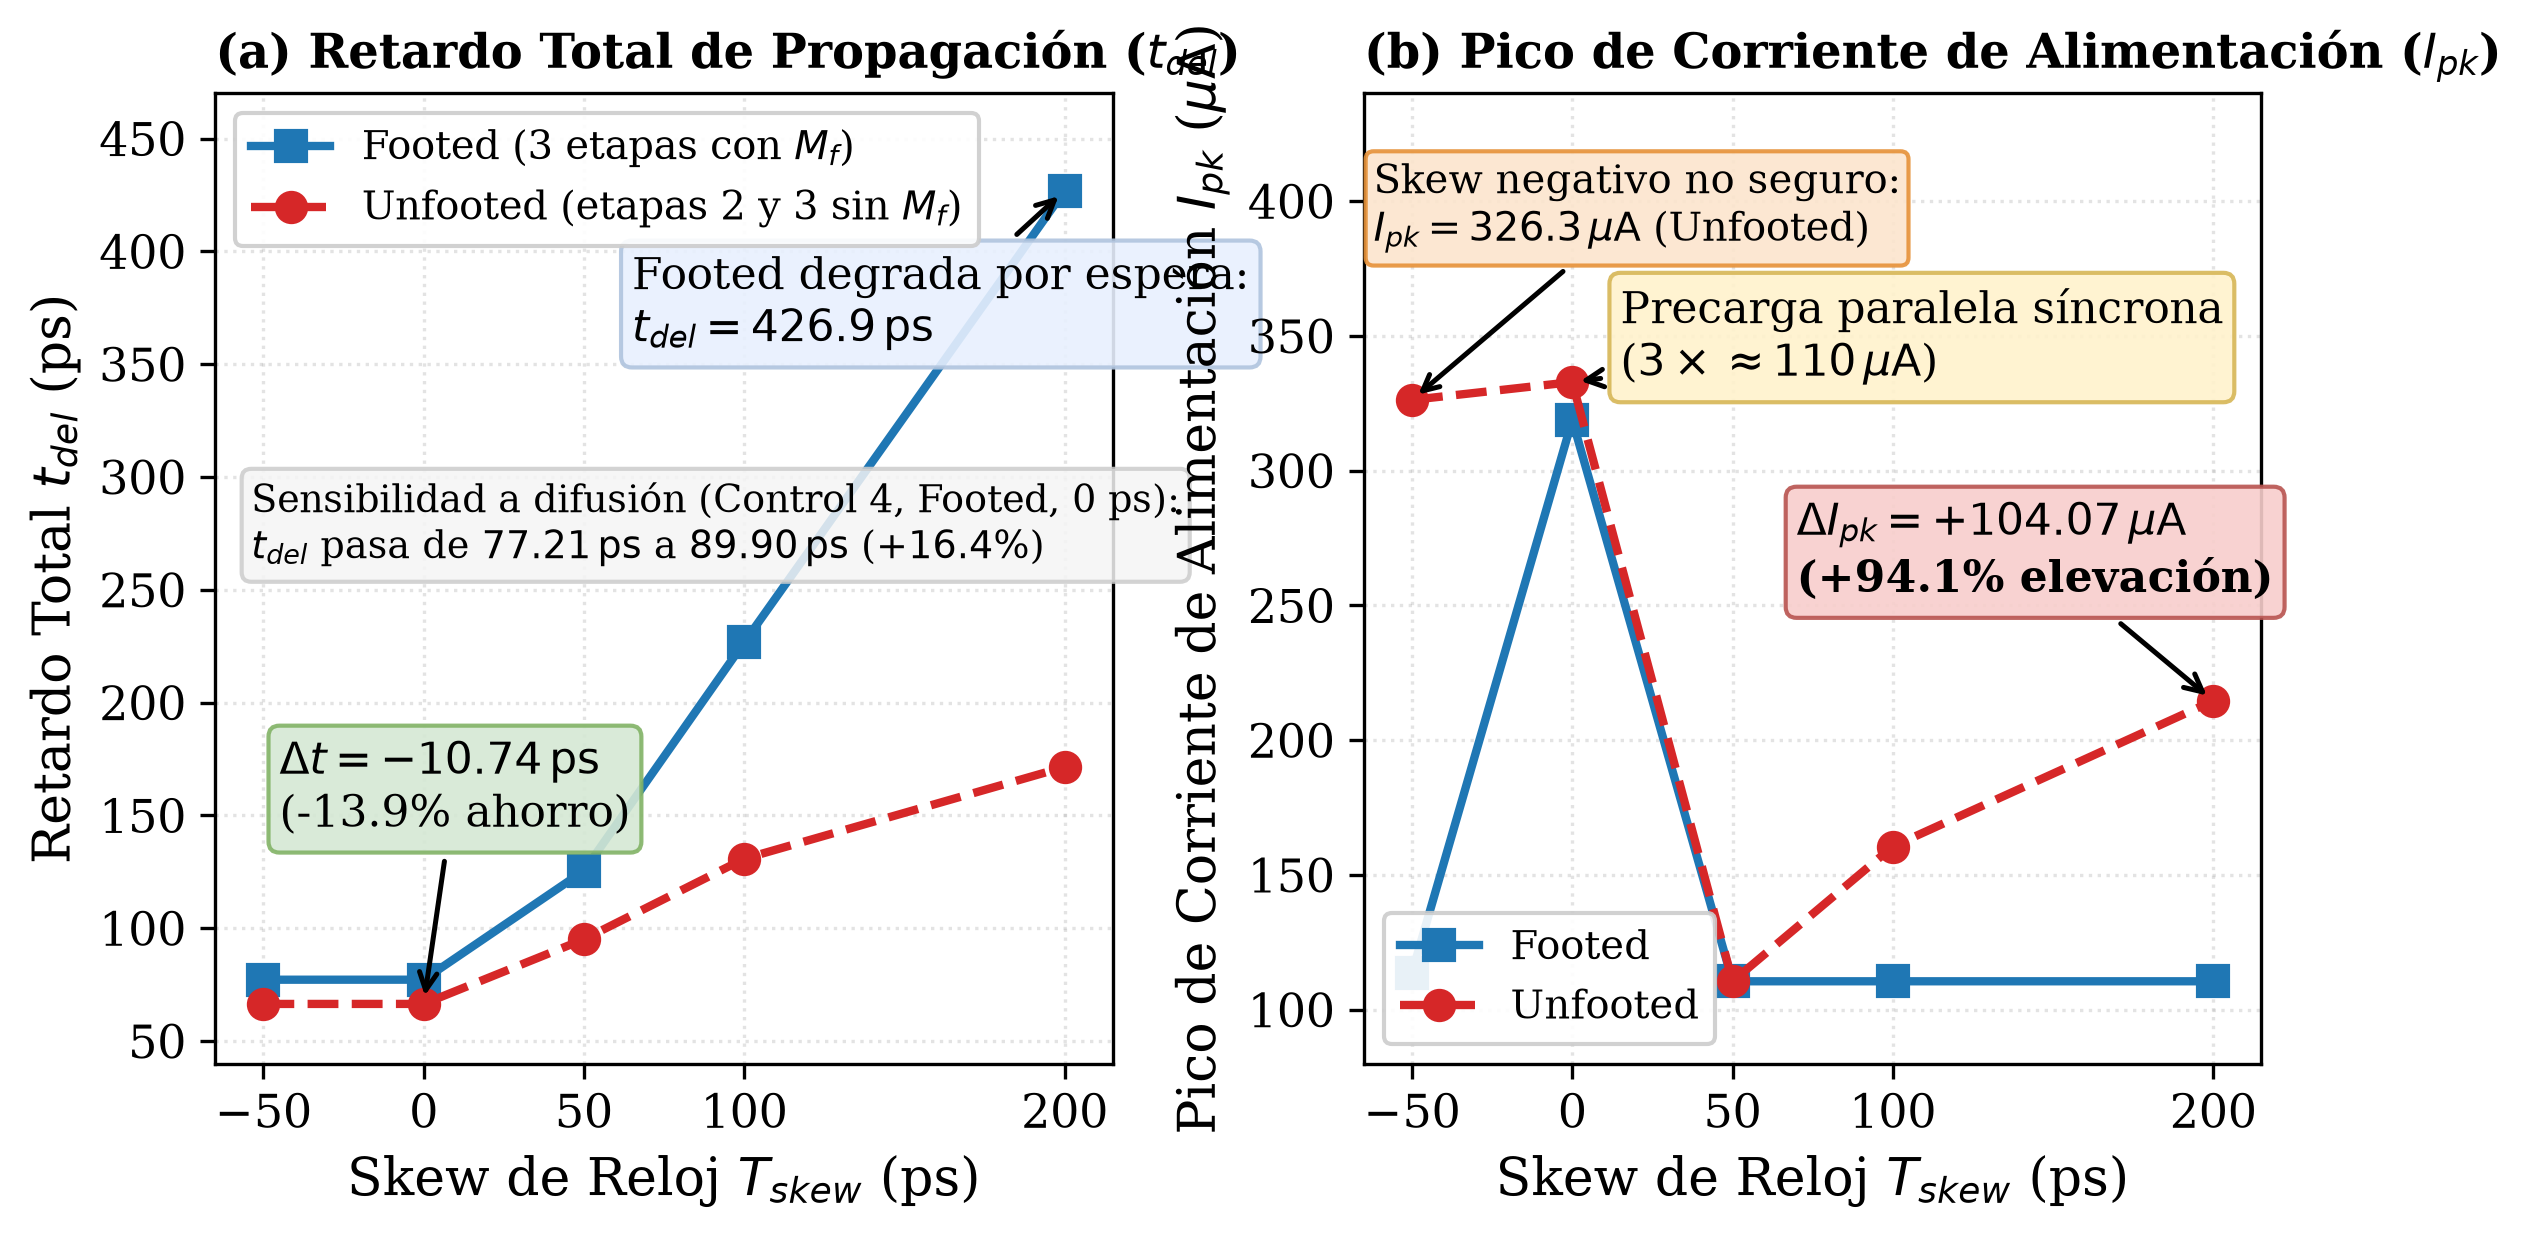
\includegraphics[width=0.55\linewidth,height=2.7cm,keepaspectratio]{figuras/fig3_act4_footed_vs_unfooted_skew.png}
  \caption[Sensibilidad al skew de reloj en cascada dominó de 3 etapas]{Sensibilidad al skew de reloj en cascada dominó de 3 etapas (PTM 45\,nm HP): (a) Retardo total de propagación $t_{\text{del}}$ vs $T_{\text{skew}}$; (b) Pico de corriente de alimentación $I_{\text{pk}}$ vs $T_{\text{skew}}$.}
  \label{fig:footed_vs_unfooted_skew}
\end{figure}

\subsection{Conclusiones de la Actividad 4}
\begin{enumerate}[leftmargin=1.4em,itemsep=0.0em]
  \item \textbf{Eficacia del Inversor Dominó:} La cascada directa sin inversor sufre una descarga espuria de $353.76\,\text{mV}$ ($\Delta NM_H = -84\%$) por activación prematura de la PDN. El inversor estático asegura transiciones monótonas crecientes ($0 \to 1$), garantizando retención íntegra de $V_{DD}$ ante $X=0$ y conmutación activa funcional cuando $X=1$.
  \item \textbf{Monotonicidad en Entradas Externas:} La caída de una entrada externa ($X: 1 \to 0$) produce un error lógico en dicho ciclo ($out2 \approx 1.0\,\text{V}$ en vez de $0\,\text{V}$) porque la descarga precede a la transición y la carga no se repone con $CLK=1$. Esto exige que los biestables excitadores (ej. TGFF) sean rigurosamente monótonos y sin glitches.
  \item \textbf{Compromiso Footed vs Unfooted:} Prescindir del footer ahorra $13.9\%$ de retardo a skew nulo, pero a $T_{\text{skew}}=+200\,\text{ps}$ eleva el pico de alimentación en $+104.07\,\mu\text{A}$ ($+94.1\%$) y a $-50\,\text{ps}$ genera $326.30\,\mu\text{A}$. La celda Footed brinda inmunidad robusta frente a desalineamientos temporales.
\end{enumerate}

% ==============================================================================
% SECCION 6: ACTIVIDAD 5 - EFECTOS PARASITOS, FRECUENCIAS Y OPERACION NTV
% ==============================================================================
\section{Actividad 5: Efectos Parásitos, Ventana de Frecuencia y Operación en Tensión Reducida (NTV)}
\label{sec:actividad5}

En tecnologías submicrométricas profundas ($45\,\text{nm}$), el escalado de tensión hacia el régimen \textit{Near-Threshold Voltage} (NTV) y subumbral reduce drásticamente el consumo dinámico, pero exacerba los efectos parásitos de acoplamiento capacitivo y degrada los márgenes de retención frente a corrientes de fuga. Esta sección analiza el fenómeno de \textit{clock feedthrough} en el PMOS de precarga, determina experimentalmente los límites de frecuencia $[f_{\min}, f_{\max}]$ que confinan la ventana operable de la lógica dominó, contrasta los nodos PTM 45\,nm HP y LP en subumbral ($V_{DD} = 0.50\,\text{V}$) y cuantifica el escalado de energía por ciclo.

\subsection{Sobreimpulso por Clock Feedthrough, Recorte por Diodo y Amortiguamiento}
Se evaluó la respuesta transitoria del nodo dinámico durante la transición de precarga ($CLK: 1 \to 0$ con $t_r = t_f = 5\,\text{ps}$) en la compuerta NAND3 dinámica (PTM 45\,nm HP, $V_{DD} = 1.0\,\text{V}$, $C_L = 0.5\,\text{fF}$).

\begin{enumerate}[leftmargin=1.4em,itemsep=0.01em]
  \item \textbf{Mecanismo Físico y Modelo Analítico:} La capacitancia parásita compuerta-drenaje del PMOS ($W_p = 135\,\text{nm}$), $C_{gd} = (cgdo + cgdl)W_p \approx \mathbf{0.0507\,\text{fF}}$, forma un divisor capacitivo con el nodo ($C_{\text{total}} \approx 0.85\text{--}1.05\,\text{fF}$), prediciendo un sobreimpulso analítico de $\Delta V \approx V_{DD}\frac{C_{gd}}{C_{\text{total}}} \approx \mathbf{50\text{--}60\,\text{mV}}$.
  \item \textbf{Validación Experimental y Recorte Transitorio por Diodo $D_{DB}$:} Sin keeper, la simulación registra un sobreimpulso de $\mathbf{+64.31\,\text{mV}}$ ($V_{dyn,\max} = 1.0643\,\text{V}$, Figura~\ref{fig:feedthrough_energia}(a)), reproduciendo la cota experimental de referencia ($+61.30\,\text{mV}$, con desviación relativa inferior al $4.9\%$). La unión $p\text{-}n$ drenaje-sustrato entra en conducción directa transitoria con pico $I_{D_{DB},\text{pk}} = \mathbf{2.841\,\mu\text{A}}$, recortando físicamente el sobreimpulso.
  \item \textbf{Amortiguamiento Pasivo con Keeper PMOS ($W_{kp} = 45\,\text{nm}$):} La capacitancia adicional añadida por el keeper reduce pasivamente el sobreimpulso a $\mathbf{+49.31\,\text{mV}}$ ($V_{dyn,\max} = 1.0493\,\text{V}$, reducción del $\mathbf{-23.3\%}$), sin alterar la funcionalidad.
\end{enumerate}

\begin{figure}[htbp]
  \centering
  \begin{minipage}[t]{0.485\textwidth}
    \centering
    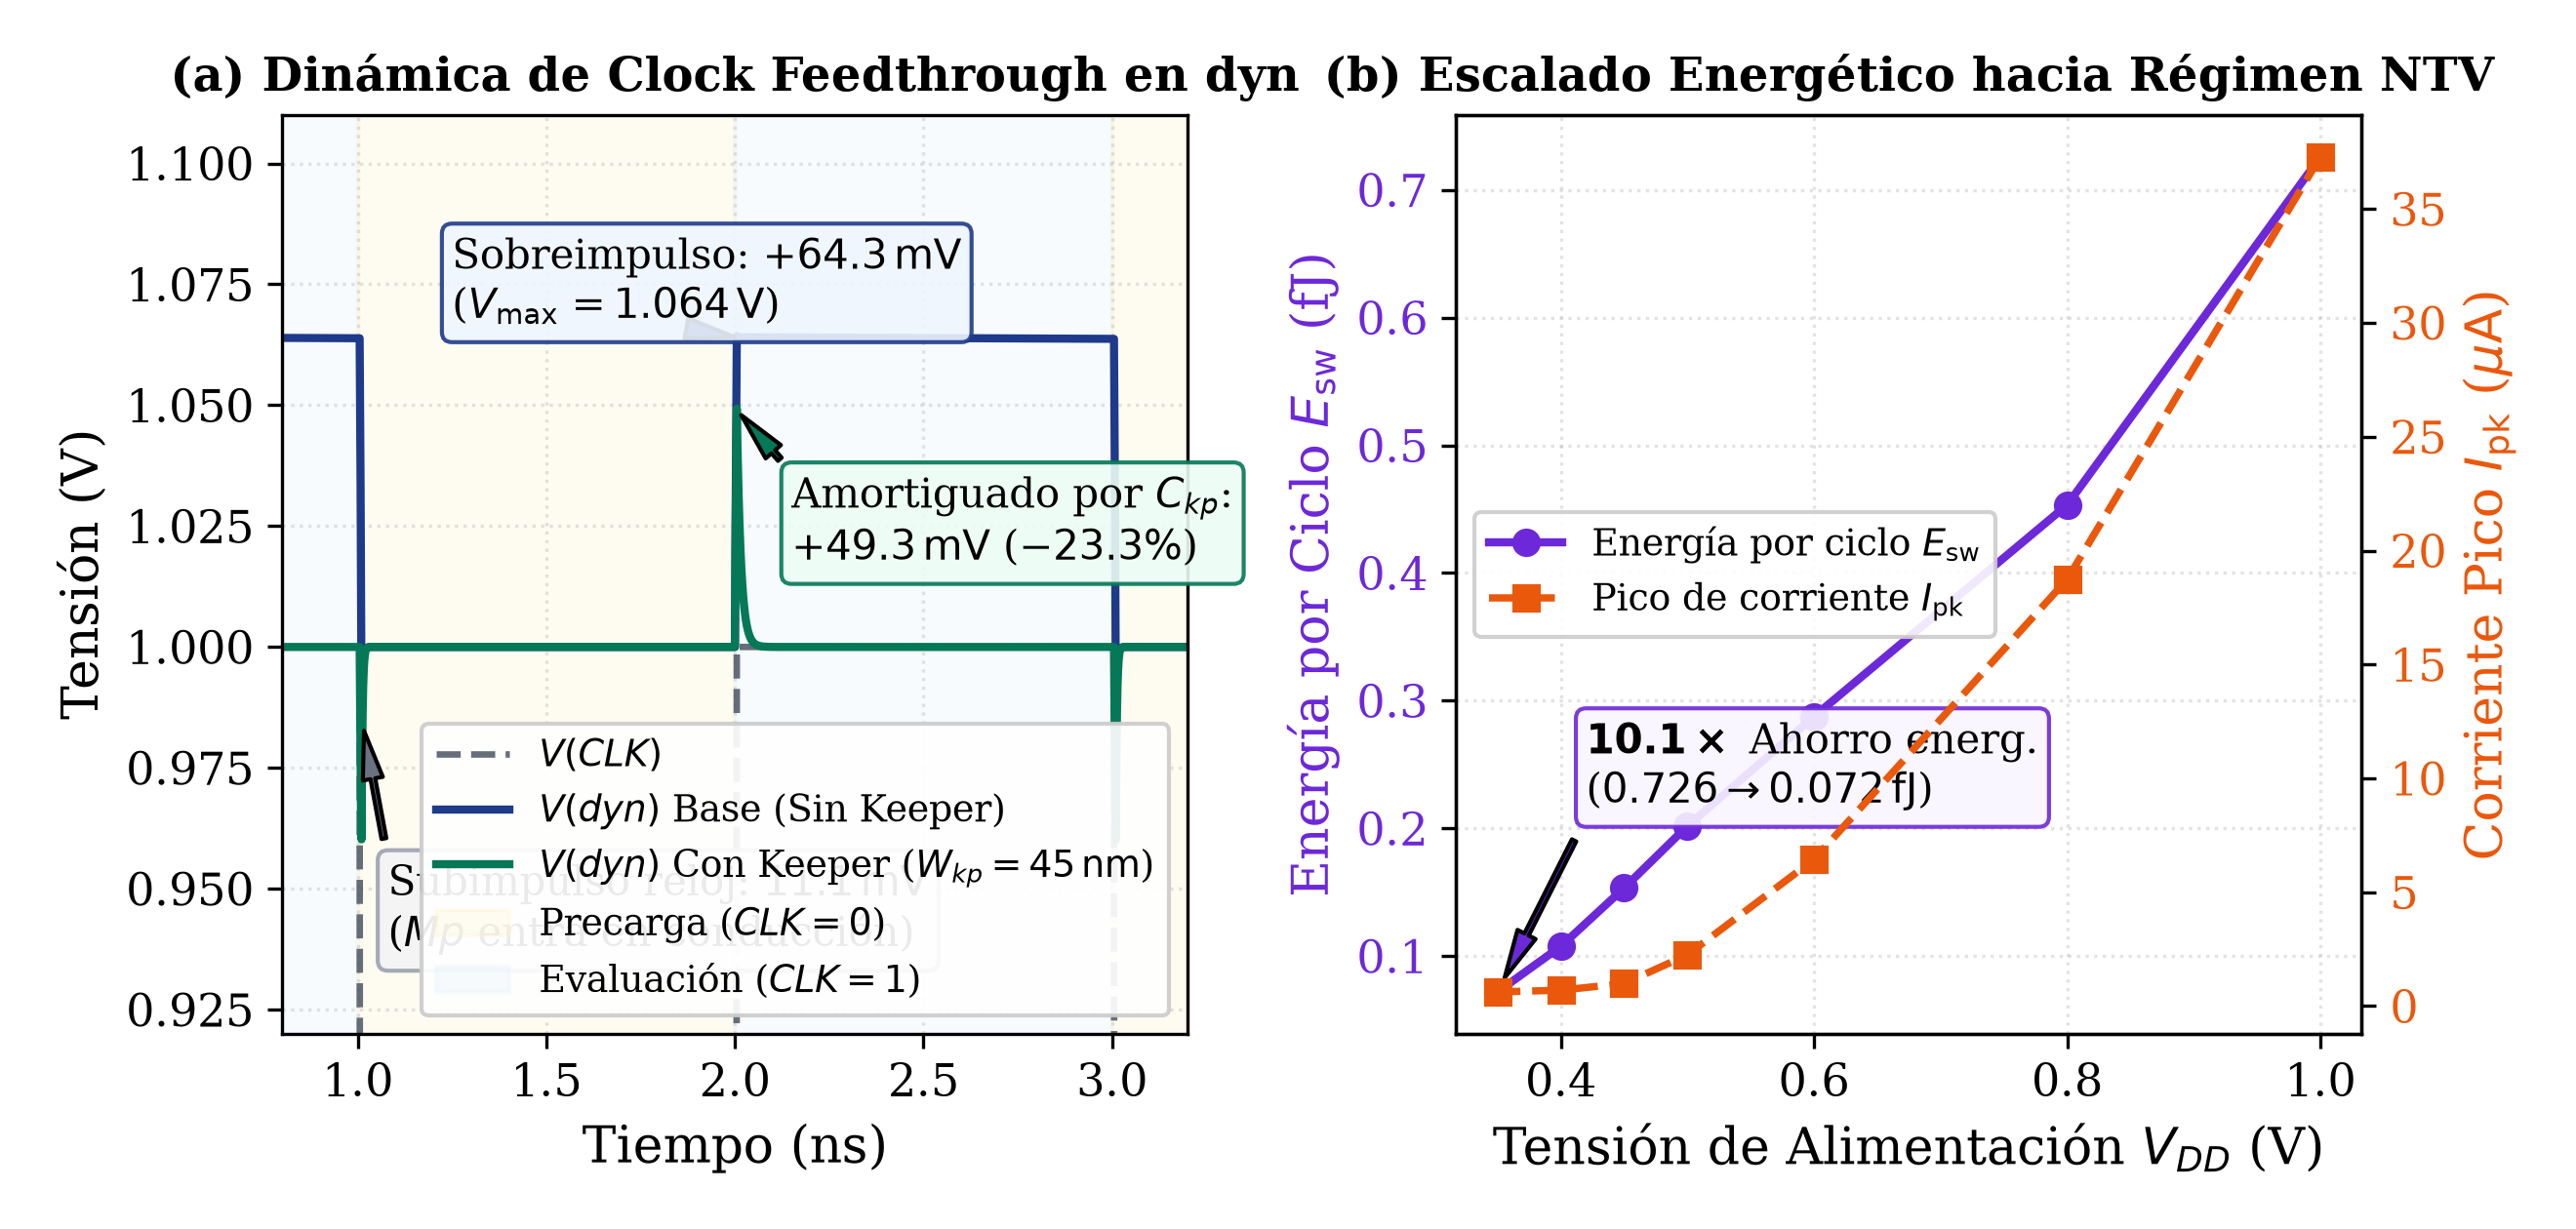
\includegraphics[width=\linewidth,height=3.0cm,keepaspectratio]{figuras/fig1_act5_feedthrough_energia.png}
    \caption[Clock feedthrough y escalado de energía]{Caracterización en PTM 45\,nm HP: (a) Feedthrough en $dyn$ con y sin keeper; (b) Escalado de $I_{\text{pk}}$ y energía dinámica $E_{\text{sw}}$ vs $V_{DD}$.}
    \label{fig:feedthrough_energia}
  \end{minipage}\hfill
  \begin{minipage}[t]{0.485\textwidth}
    \centering
    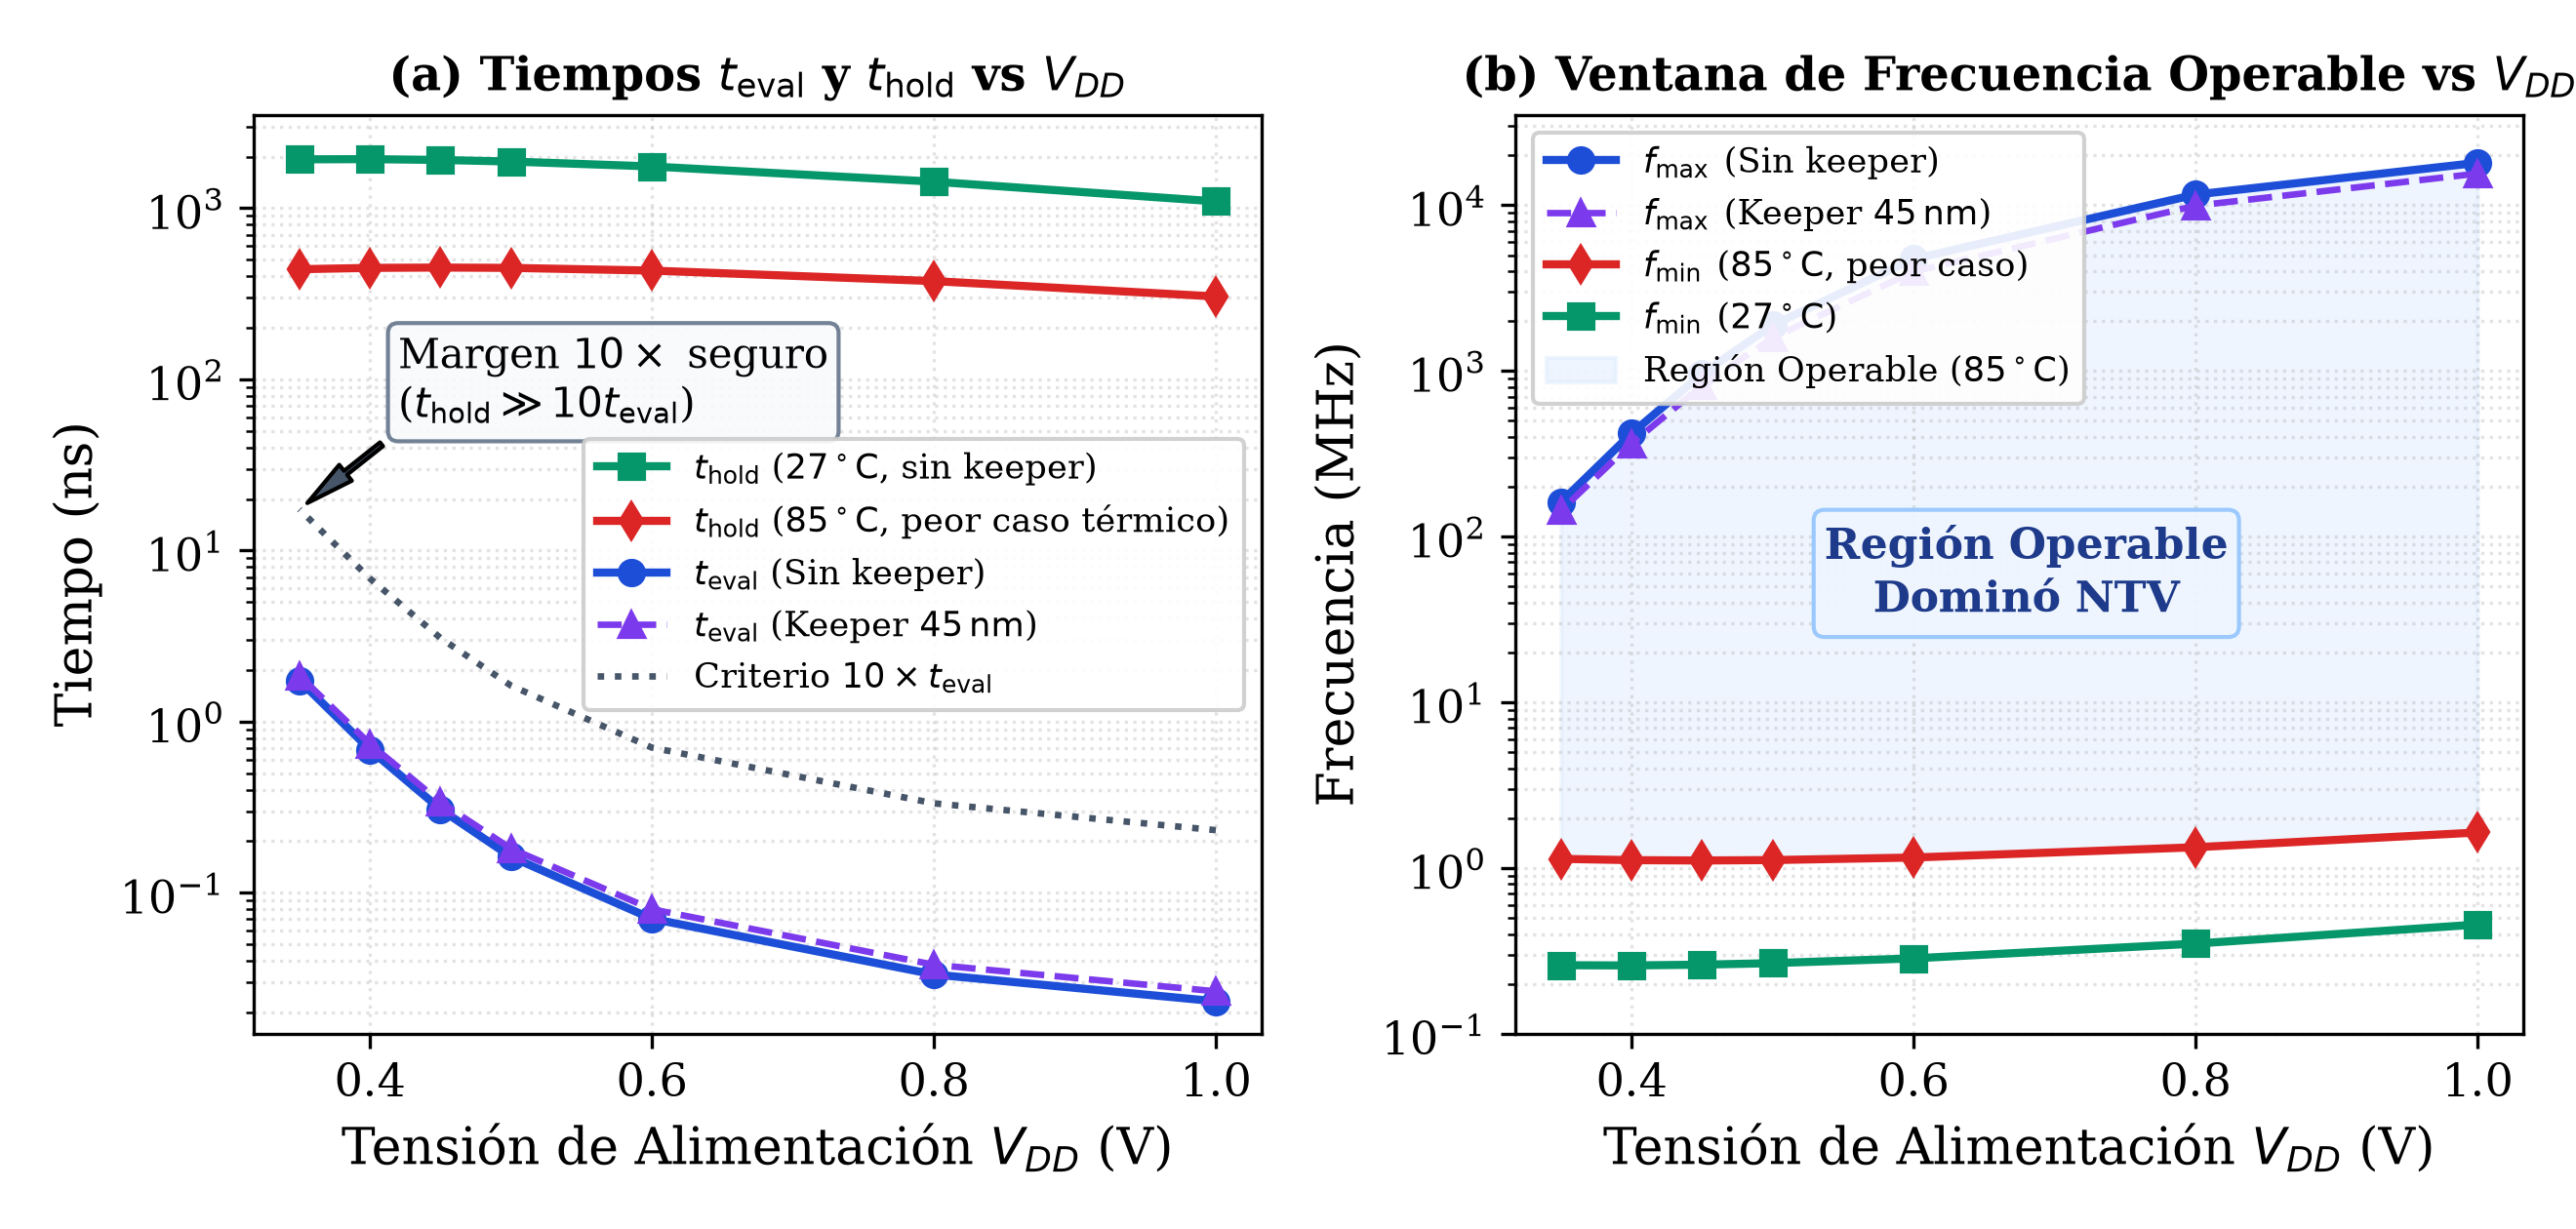
\includegraphics[width=\linewidth,height=3.0cm,keepaspectratio]{figuras/fig2_act5_ventana_frecuencia_ntv.png}
    \caption[Ventana de frecuencia operable NTV]{Frecuencia en PTM 45\,nm HP: (a) $t_{\text{eval}}$ vs $t_{\text{hold}}$ a $27^\circ\text{C}$ y $85^\circ\text{C}$; (b) Ventana operable $[f_{\min}, f_{\max}]$ en MHz reales.}
    \label{fig:ventana_ntv}
  \end{minipage}
\end{figure}

\subsection{Ventana de Frecuencia Operable \texorpdfstring{$[f_{\min}, f_{\max}]$}{[fmin, fmax]} y Operación en Régimen NTV}
La viabilidad operativa está acotada por dos cotas físicas: una frecuencia máxima $f_{\max} \approx 1/(2 \cdot t_{\text{pd}})$, derivada del retardo de la etapa completa ($t_{\text{pd}} = t_{\text{eval}} + t_{pLH,\text{inv}}$), y una frecuencia mínima $f_{\min} \approx 1/(2 \cdot t_{\text{hold}})$, impuesta por la fuga estática. Se precisa que $f_{\max}$ es una \textbf{cota analítica superior estimada desde el retardo transitorio}, no una oscilación periódica sostenida.

\begin{itemize}[leftmargin=1.4em,itemsep=0.01em]
  \item \textbf{Cota Superior ($f_{\max}$) y Penalización por Contención en NTV:} A $V_{DD}=1.0\,\text{V}$, la etapa dominó conmuta en $t_{\text{pd}} = 27.72\,\text{ps} \implies f_{\max} = \mathbf{18.035\,\text{GHz}}$ ($t_{\text{eval}}=33.56\,\text{ps}$ en celda aislada sin carga de inversor). A $0.35\,\text{V}$, la pérdida de sobremarcha eleva el retardo a $t_{\text{pd}} = 3087.20\,\text{ps} \implies f_{\max} = \mathbf{161.96\,\text{MHz}}$. La contención de un keeper de $45\,\text{nm}$ incrementa $t_{\text{pd}}$ a $32.20\,\text{ps}$ ($15.53\,\text{GHz}$) en $1.0\,\text{V}$ y a $3468.80\,\text{ps}$ ($144.14\,\text{MHz}$) en $0.35\,\text{V}$ ($+12.4\%$).
  \item \textbf{Cota Inferior ($f_{\min}$) e Impacto Térmico:} En $1.0\,\text{V}$, la fuga subumbral ($27^\circ\text{C}$) fija $t_{\text{hold}} = 1.096\,\mu\text{s} \implies f_{\min} = \mathbf{456.21\,\text{kHz}}$ ($447.23\,\text{kHz}$ en ensayo de referencia previo). A $85^\circ\text{C}$, las fugas térmicas contraen la retención a $t_{\text{hold}} = 0.305\,\mu\text{s}$ ($1.0\,\text{V}$) y $0.440\,\mu\text{s}$ ($0.35\,\text{V}$), elevando $f_{\min}$ a $\mathbf{1.639\,\text{MHz}}$ y $\mathbf{1.136\,\text{MHz}}$ (aceleración de $\sim 3.6\times$).
  \item \textbf{Criterio de Seguridad $t_{\text{hold}} \ge 10 \cdot t_{\text{eval}}$:} En todo el rango caracterizado ($V_{DD} \in [0.35, 1.00]\,\text{V}$), la ventana operable $[f_{\min}, f_{\max}]$ \textbf{permanece abierta} (Figura~\ref{fig:ventana_ntv}(b)), con $f_{\max}/f_{\min} = 142\times$ y $t_{\text{hold}}/t_{\text{eval}} = 1\,109 \gg 10$ en el peor caso ($0.35\,\text{V}$, $85^\circ\text{C}$).
  \item \textbf{Precisión Metodológica sobre $0.25\,\text{V}$ y $0.30\,\text{V}$:} Las pruebas de retención confirmaron retenciones válidas a $0.30\,\text{V}$ ($1.89\,\mu\text{s}$) y $0.25\,\text{V}$ ($1.80\,\mu\text{s}$), pero al no evaluarse retardo activo ni energía por debajo de $0.35\,\text{V}$, la ventana formal completa se delimita rigurosamente en $[0.35, 1.00]\,\text{V}$.
  \item \textbf{Retención con Keeper:} Con keeper ($W_{kp} \in \{45, 90\}\,\text{nm}$), el equilibrio $I_{kp} \approx I_{\text{sub}}$ mantiene caída $<0.6\,\text{mV}$ en $15\,\mu\text{s}$, fijando una cota inferior observada $t_{\text{hold}} > 15\,\mu\text{s} \implies f_{\min} < \mathbf{33.3\,\text{kHz}}$.
\end{itemize}

\begin{table}[htbp]
\centering
\fontsize{7.5pt}{8.8pt}\selectfont
\caption[Consolidación de métricas de conmutación, retención y energía en NTV]{Consolidación experimental en régimen NTV (PTM 45\,nm HP, $C_L=0.5\,\text{fF}$): retardo de evaluación, frecuencias operables estimadas ($f_{\max}$ calculada desde $t_{\text{pd}}$) y escalado de energía.}
\label{tab:ntv_resumen}
\begin{tabularx}{\linewidth}{@{}>{\centering\arraybackslash}p{1.0cm} >{\centering\arraybackslash}p{1.2cm} >{\centering\arraybackslash}p{1.2cm} >{\centering\arraybackslash}p{1.3cm} >{\centering\arraybackslash}p{1.4cm} >{\centering\arraybackslash}p{1.4cm} >{\centering\arraybackslash}p{1.3cm} >{\centering\arraybackslash}p{1.3cm} >{\RaggedRight\arraybackslash}X@{}}
\toprule
\textbf{$V_{DD}$} & \textbf{$t_{\text{eval}}$} & \textbf{$t_{\text{pd}}$} & \textbf{$f_{\max}$ Act5} & \textbf{$t_{\text{hold}}$ 27°C} & \textbf{$f_{\min}$ 27°C} & \textbf{$f_{\min}$ 85°C} & \textbf{Energía} & \textbf{Diagnóstico y Margen} \\
\textbf{(V)} & \textbf{(ps)} & \textbf{(ps)} & \textbf{(GHz)} & \textbf{($\mu\text{s}$)} & \textbf{(kHz)} & \textbf{(MHz)} & \textbf{($E_{\text{sw}}$, fJ)} & \textbf{de Seguridad ($t_{\text{hold}}/t_{\text{eval}}$)} \\
\midrule
$1.00$ & $23.21$  & $27.72$   & $\mathbf{18.035}$ & $1.096$ & $456.2$ & $1.64$ & $0.7259$ & Nominal HP ($47\,200 \gg 10$). \\
$0.80$ & $33.31$  & $43.11$   & $\mathbf{11.599}$ & $1.429$ & $349.9$ & $1.33$ & $0.4533$ & Retardo $+55\%$, energía $-38\%$. \\
$0.60$ & $70.48$  & $105.40$  & $\mathbf{4.744}$  & $1.754$ & $285.0$ & $1.16$ & $0.2876$ & Balance óptimo energía-retardo. \\
$0.50$ & $162.34$ & $264.52$  & $\mathbf{1.890}$  & $1.874$ & $266.7$ & $1.12$ & $0.2018$ & Régimen NTV ($11\,543 \gg 10$). \\
$0.45$ & $308.17$ & $520.47$  & $\mathbf{0.961}$  & $1.914$ & $261.2$ & $1.11$ & $0.1533$ & Transición a subumbral. \\
$0.40$ & $686.10$ & $1191.33$ & $\mathbf{0.420}$  & $1.935$ & $258.4$ & $1.12$ & $0.1076$ & $f_{\max} = 420\,\text{MHz} \gg f_{\min}$. \\
$0.35$ & $1739.95$& $3087.20$ & $\mathbf{0.162}$  & $1.930$ & $259.1$ & $1.14$ & $0.0719$ & Subumbral: $E_{\text{sw}}$ $-90.1\%$ ($1109 \gg 10$). \\
\bottomrule
\end{tabularx}
\end{table}

\subsection{Comparativa Subumbral a \texorpdfstring{$V_{DD} = 0.50\,\text{V}$}{VDD = 0.50 V}: 45nm HP vs 45nm LP y Energía}
Bajo polarización idéntica a $V_{DD} = 0.50\,\text{V}$ ($T=27^\circ\text{C}$, $C_L=0.5\,\text{fF}$), se contrastó el desempeño subumbral entre las variantes de alto rendimiento (HP) y bajo consumo (LP):

\begin{itemize}[leftmargin=1.4em,itemsep=0.01em]
  \item \textbf{Corrientes y Selectividad:} En 45nm LP, el mayor espesor de óxido (en NMOS: $t_{oxe} = 1.80\,\text{nm}$, $t_{oxp}=1.50\,\text{nm}$, $d_{tox}=0.30\,\text{nm}$ vs $1.25\,\text{nm}$, $1.00\,\text{nm}$, $0.25\,\text{nm}$ en HP; en PMOS $t_{oxe}=1.82\,\text{nm}$ vs $1.30\,\text{nm}$) y $V_{thn} = 0.623\,\text{V} > V_{DD}$ reducen la fuga $I_{\text{off}}$ a $\mathbf{0.671\,\text{pA}}$ vs $\mathbf{125.05\,\text{pA}}$ en HP ($\mathbf{186.4\times}$ menor fuga). La selectividad $I_{\text{on}}/I_{\text{off}}$ asciende a $146\,950$ ($3.75\times$ superior a HP).
  \item \textbf{Compromiso de Retardo:} La menor corriente activa en LP ($98.6\,\text{nA}$ vs $4.898\,\mu\text{A}$) incrementa el retardo a $t_{\text{eval,LP}} = \mathbf{8488.41\,\text{ps}}$ frente a $\mathbf{161.57\,\text{ps}}$ en HP ($\mathbf{52.54\times}$ más lento; $8647.61\,\text{ps}$ en ensayo de celda aislada, apenas $1.8\%$ de discrepancia).
  \item \textbf{Escalado de Energía por Ciclo ($E_{\text{sw}}$):} La integración de corriente en $10\,\text{ns}$ demuestra una reducción de $E_{\text{sw}} = \mathbf{0.7259\,\text{fJ}}$ a $1.0\,\text{V}$ ($I_{\text{pk}} = 37.29\,\mu\text{A}$) hasta $\mathbf{0.0719\,\text{fJ}}$ a $0.35\,\text{V}$ ($I_{\text{pk}} = 0.62\,\mu\text{A}$), logrando un ahorro energético del $\mathbf{90.1\%}$ ($\mathbf{10.1\times}$ de reducción, Tabla~\ref{tab:ntv_resumen}).
\end{itemize}

\subsection{Conclusiones de la Actividad 5}
\begin{enumerate}[leftmargin=1.4em,itemsep=0.01em]
  \item \textbf{Amortiguamiento del Feedthrough:} El sobreimpulso por acoplamiento capacitivo ($+64.31\,\text{mV}$) queda acotado pasivamente por el diodo $D_{DB}$ y se atenúa un $23.3\%$ ($+49.31\,\text{mV}$) por la capacitancia intrínseca añadida por el keeper PMOS.
  \item \textbf{Viabilidad de Lógica Dominó en NTV:} La lógica dominó es viable en tensiones reducidas ($V_{DD} \ge 0.35\,\text{V}$) preservando una ventana operable de $[1.14\,\text{MHz}, 161.96\,\text{MHz}]$ a $85^\circ\text{C}$ con holgura $t_{\text{hold}} \gg 10 \cdot t_{\text{eval}}$. Su coste respecto a la lógica estática radica en una mayor sensibilidad al ruido y la necesidad imperiosa de un keeper dimensionado para evitar el vaciado subumbral ante detenciones de reloj.
  \item \textbf{Compromiso Tecnológico HP vs LP:} El nodo LP proporciona una selectividad $I_{\text{on}}/I_{\text{off}}$ $3.75\times$ superior con fugas $186\times$ menores, garantizando retención estática sin keeper, pero sufre una severa penalización de velocidad ($52.5\times$ más lenta) que restringe su uso a sistemas de baja frecuencia.
\end{enumerate}

% ==============================================================================
% SECCION 7: CUESTIONARIO
% ==============================================================================
\section{Cuestionario}
\label{sec:cuestionario}

\begin{enumerate}[leftmargin=1.5em,itemsep=0.04em,parsep=0pt,topsep=0.1em]

\item \textbf{Imposibilidad de transición $0 \to 1$ en evaluación:} En evaluación ($CLK=1$), el PMOS de precarga está apagado ($V_{GS,p}=0\,\text{V}$). El nodo dinámico $dyn$ es puramente capacitivo y carece de trayectoria hacia $V_{DD}$; por ende, no puede recargarse. Solo puede conservar $V_{DD}$ (PDN en corte) o descargarse a tierra ($1 \to 0$, PDN activa). El \textit{clock feedthrough} acopla sobreimpulsos transitorios, pero la celda es incapaz de generar una transición lógica ascendente $0 \to 1$.

\item \textbf{Capacitancia de entrada (dinámica vs estática):} En CMOS estático, la entrada conmuta compuertas NMOS y PMOS en paralelo ($C_{\text{in}} = C_{gn} + C_{gp}$); en dominó, la señal excita únicamente transistores NMOS ($C_{\text{in}} = C_{gn}$), asumiendo el reloj la precarga PMOS. En la NAND3 caracterizada ($W_n = 270\,\text{nm}, W_p = 135\,\text{nm}$), suprimir la rama PMOS reduce la capacitancia de entrada en SPICE un $42.4\%$ ($0.3417\,\text{fF}$ vs $0.5936\,\text{fF}$), aliviando significativamente el esfuerzo y retardo del excitador.

\item \textbf{Factor de actividad $\alpha \approx 1$ e implicancias en potencia:} El nodo $dyn$ se precarga a $V_{DD}$ cada ciclo ($CLK=0$). Si las entradas activan la PDN, $dyn$ se descarga en cada evaluación ($CLK=1$), imponiendo $\alpha = 1$ aun con datos constantes. Con baja actividad de datos (donde estático ahorra con $\alpha < 0.1$), la lógica dinámica disipa continuamente potencia de reloj y conmutación ($P = \alpha C_L (V_{DD})^2 f$), perdiendo competitividad energética.

\item \textbf{Deducción de $\Delta V$ y condición de corte por $V_{th}$:} Por balance de carga con nodo interno en cero: $Q_0 = C_L V_{DD} = (C_L+C_a)V_f \implies \Delta V = [C_a/(C_a+C_L)]V_{DD}$. Esta relación deja de ser válida si el NMOS se estrangula antes de igualar potenciales ($V_{GS} < V_{th}$), condición que ocurre cuando $V_{th,\text{eff}} > [C_a/(C_a+C_L)]V_{DD}$. Al cortarse en $V_a = V_{DD} - V_{th,\text{eff}}$, cesa la redistribución y la caída efectiva queda acotada por $\Delta V = (C_a/C_L)(V_{DD} - V_{th,\text{eff}})$.

\item \textbf{Orden de apilamiento en PDN dinámica vs estática:} En lógica estática, el nivel final $V_{OL}$ solo exige conducción DC a tierra, siendo indiferente el orden de apilamiento. En lógica dinámica, $dyn$ flota en alta impedancia; situar las entradas activas en transistores superiores contiguos a $dyn$ conecta de inmediato capacitancias de difusión parásitas no precargadas, maximizando el \textit{charge sharing}. Situar el transistor en corte arriba aísla la carga interna y preserva $V_{dyn}$.

\item \textbf{Regla de monotonicidad dominó y rol del inversor:} En evaluación ($CLK=1$), las entradas a la PDN solo deben realizar transiciones $0 \to 1$ (o reposar en 0). Como $dyn$ parte de $V_{DD}$ y solo puede caer ($1 \to 0$), conectarlo directo causaría la descarga espuria inmediata de la etapa siguiente antes de que evalúe. El inversor estático complementa la señal ($out: 0 \to 1$), manteniendo la PDN receptora apagada durante precarga y activándola monótonamente solo tras evaluar.

\item \textbf{Funciones no realizables en dominó y soluciones:} La lógica dominó estándar es no inversora ($dyn \downarrow \implies out \uparrow$), impidiendo realizar funciones complementarias directas (NAND, NOR, XOR) en una sola etapa. Se soluciona mediante: (1) \textit{Dual-Rail Domino} (DCVSL), que genera a la vez $F$ y $\overline{F}$ con PDNs diferenciales complementarias; y (2) \textit{NP-Domino} (Zipper), alternando etapas n-dominó y p-dominó con relojes en oposición.

\item \textbf{Corriente subumbral y mayor $nfactor$ en 45nm HP vs LP:} La corriente subumbral escala como $I_{\text{sub}} \propto (n-1)\exp[(V_{GS}-V_{th})/(n k T/q)][1 - \exp(-V_{DS}/(kT/q))]$. El factor $n = 1 + C_{\text{dep}}/C_{\text{ox}}$ refleja el acoplamiento capacitivo compuerta-canal. En 45nm HP, el dopaje \textit{halo} severo para mitigar DIBL eleva $C_{\text{dep}}$ frente a $C_{\text{ox}}$, incrementando $n$ ($1.53$ vs $1.15$ en LP). Un mayor $n$ degrada la pendiente subumbral ($S = n(kT/q)\ln 10$), disparando la fuga $I_{\text{off}}$.

\item \textbf{Comparativa 45nm HP vs LP en lógica dinámica:} LP presenta óxido más grueso ($t_{oxp}=1.50\,\text{nm}$; $t_{oxe}=1.80\,\text{nm}/1.82\,\text{nm}$, $d_{tox}=0.30/0.32\,\text{nm}$ en NMOS/PMOS vs $t_{oxp}=1.00\,\text{nm}$, $t_{oxe}=1.25/1.30\,\text{nm}$, $d_{tox}=0.25/0.30\,\text{nm}$ en HP), mayor umbral ($0.623\,\text{V}$ vs $0.469\,\text{V}$) y fuga $186\times$ menor ($0.67\,\text{pA}$ vs $125.1\,\text{pA}$), reteniendo carga a 85°C ($1\,\mu\text{s}$, $\Delta V < 2\,\text{mV}$) sin keeper. Empero, conmuta $52.5\times$ más lento: LP prima en retención y HP en velocidad.

\item \textbf{Keeper condicional y contención:} El keeper PMOS mitiga fugas y \textit{charge sharing}, pero disputa corriente con la PDN en evaluación, demorando la conmutación ($+12.90\%$ en 45nm HP con $W_{kp}=45\,\text{nm}$). El keeper condicional reduce esta penalización: retiene con un transistor mínimo en reposo y desconecta la rama mayor mediante reloj retardado durante la evaluación activa, reduciendo la demora a solo $+5.11\%$ y asegurando retención a 85°C.

\pagebreak
\item \textbf{Realimentación de keeper desde la salida del inversor:} El keeper PMOS restaura $V_{DD}$ en $dyn$; para encenderlo, su compuerta requiere $0\,\text{V}$. Conectar la compuerta directamente a $dyn$ lo mantendría apagado ($V_G=V_S=V_{DD}$). La salida invertida $out = \overline{dyn}$ provee la polaridad complementaria requerida. Asimismo, la alta ganancia regenerativa del inversor proporciona conmutación abrupta y desacopla la compuerta del keeper de perturbaciones transitorias en el nodo flotante.

\item \textbf{Clock feedthrough, origen en PMOS y dependencia con $dV/dt$:} El \textit{clock feedthrough} es el acoplamiento capacitivo del flanco de reloj al nodo flotante $dyn$ vía la capacitancia de solapamiento $C_{gd} = (c_{gdo}+c_{gdl})W_p$ del PMOS de precarga. La corriente inyectada es $i = C_{gd}(dV_{\text{clk}}/dt)$; flancos más abruptos (menor $t_r, t_f$) elevan $dV/dt$, inyectando un sobreimpulso ($+64.3\,\text{mV}$ en 45nm HP) que es recortado por conducción del diodo drenaje-sustrato $D_{DB}$ del PMOS.

\item \textbf{Skew positivo tolerable en footed vs cortocircuito en unfooted:} En dominó \textit{Footed}, el transistor de pie $M_f$ aísla la PDN hasta la llegada de su reloj local $CLK2$; si $T_{\text{skew}}>0$, la conmutación se retrasa pero sin degradar la lógica. En \textit{Unfooted}, la PDN conecta directo a masa; si la etapa previa inicia precarga ($CLK1: 1 \to 0$) mientras la receptora continúa en evaluación ($CLK2=1$), PMOS y PDN conducen simultáneamente, creando un cortocircuito $V_{DD} \to \text{GND}$ ($+94.1\%$ en corriente).

\item \textbf{Restricción de $f_{\min}$ en lógica dinámica vs estática:} El nodo dinámico almacena el estado como carga en un condensador flotante; las fugas subumbral y GIDL drenan esta carga en un tiempo finito $t_{\text{hold}}$, fijando una cota inferior de reloj $f \ge f_{\min} \approx 1/(2t_{\text{hold}})$ para evitar cruzar el umbral $V_M$. La lógica CMOS estática carece de límite inferior ($f_{\min}=0\,\text{Hz}$) porque sus salidas están conectadas permanentemente a los rieles de alimentación mediante trayectorias óhmicas.

\item \textbf{Degradación exponencial de $I_{\text{on}}/I_{\text{off}}$ en NTV:} Al reducir $V_{DD}$ hacia $V_{th}$, la corriente activa decae exponencialmente con la sobremarcha ($I_{\text{on}} \propto \exp[(V_{DD}-V_{th})/(n k T/q)]$), mientras la fuga $I_{\text{off}}$ se reduce marginalmente, colapsando el cociente $I_{\text{on}}/I_{\text{off}}$. La lógica dinámica es hipersensible a esto porque requiere $I_{\text{on}}$ alto para evaluar y $I_{\text{off}}$ ínfimo para retener, contrayendo el margen entre $t_{\text{eval}}$ y $t_{\text{hold}}$.

\item \textbf{Inviabilidad sin keeper a $0.4\,\text{V}$ y 85°C:} Aunque la ventana periódica abre ($t_{\text{hold}}=448\,\text{ns} \gg t_{\text{eval}}$), falla por dos causas: (1) Fugas térmicas degradan $dyn$ impidiendo pausas $\Delta t > 448\,\text{ns}$ ($V_{dyn} < V_{DD}/2$); y (2) Sin restauración activa colapsa $NM_H$, dejando al nodo vulnerable a ruido capacitivo.

\item \textbf{Imprescindibilidad de $AS/AD/PS/PD$ en BSIM4:} Los parámetros $AS, AD, PS, PD$ especifican áreas y perímetros de difusión para calcular las capacitancias de juntura parásitas ($C_j, C_{jsw}, C_{jswg}$). Al omitirse en SPICE, el simulador asigna cero ($C_{\text{diff}}=0$), modelando únicamente solapamientos de compuerta ($C_{gd}, C_{gs}$). Esto subestima la capacitancia parásita interna en $80\%\text{--}95\%$, enmascarando casi por completo el \textit{charge sharing} ($\Delta V \approx 0$ en vez de $164\,\text{mV}$).

\item \textbf{Necesidad de \texttt{gmin} y \texttt{abstol} en nodos flotantes:} En estática, las bajas impedancias ($k\Omega$) toleran valores estándar. En dominó, $dyn$ flota con impedancias de teraohmios ($T\Omega$). El parámetro por defecto $\texttt{gmin}=1\text{e-}12$ inserta una conductancia espuria que drena picoamperios artificiales, falseando la retención; calibrar a $\texttt{gmin}=1\text{e-}15$ y $\texttt{abstol}=1\text{e-}14$ asegura que las fugas medidas reflejen la física BSIM4 y no tolerancias del solver.

\item \textbf{Relación dominó con TGFF imperfecto (Bappy et al., SOCC 2026):} Las compuertas dominó exigen a las etapas secuenciales excitadoras niveles estables o transiciones monótonas ($0 \to 1$) en evaluación. El TGFF propuesto por Bappy, Zhao y Han (SOCC 2026 [5]) sustituye compuertas de transmisión balanceadas por transistores de paso para NTV; esto introduce caídas $V_{th}$ y rebotes capacitivos que pueden encender falsamente la PDN receptora o degradar la evaluación dominó.

\item \textbf{Efecto cuerpo en PDN apilada y viabilidad en bulk:} En transistores apilados, los nodos internos suben ($V_S > 0\,\text{V}$), polarizando el sustrato en reversa ($V_{SB}>0\,\text{V}$) y elevando el umbral: $\Delta V_{th} = \gamma(\sqrt{2\phi_F + V_{SB}} - \sqrt{2\phi_F})$, lo que merma la sobremarcha y retarda la evaluación. Conectar sustrato a fuente anularía el efecto, pero es inviable en procesos \textit{bulk} con pozo/sustrato común; mitigarlo exige triple-well o SOI.

\end{enumerate}


% ==============================================================================
% SECCION 8: CONCLUSIONES GENERALES DEL LABORATORIO DIRIGIDO N.o 2
% ==============================================================================
\clearpage
\section{Conclusiones Generales}
\label{sec:conclusiones}

El desarrollo experimental del Laboratorio Dirigido N.\textsuperscript{o}~2 permite formular las siguientes conclusiones fundamentales de diseño en lógica CMOS dinámica submicrométrica (PTM 45\,nm):

\begin{enumerate}[leftmargin=1.5em,itemsep=0.03em,parsep=0pt,topsep=0.05em]
  \item \textbf{Asimetría Temporal y Capacitancia de Entrada:} La lógica dinámica suprime la red PMOS en datos, reduciendo la capacitancia de entrada medida en un $42.4\%$ ($0.3417\,\text{fF}$ vs $0.5936\,\text{fF}$ en SPICE). La celda dominó completa conmuta en $t_{\text{pd,eval}} = 35.89\,\text{ps}$ (disparada por reloj $CLK\uparrow$), frente a $9.61\,\text{ps}$ de la compuerta estática (disparada por dato $A\uparrow$), imponiendo la latencia fija del semiciclo de precarga.
  \item \textbf{Factor de Actividad y Coste Energético de Reloj:} La precarga cíclica incondicional impone un factor de conmutación $\alpha = 1$ en el nodo dinámico ante datos evaluados, disipando potencia ($P = \alpha C_L (V_{DD})^2 f$) y consumiendo reloj continuamente aun cuando las entradas lógicas permanezcan estáticas ($2.73\,\mu\text{W}$ vs $1.70\,\text{nW}$ estático a $V_{DD}=1.0\,\text{V}$). La ventaja energética de la lógica dinámica se restringe a rutas críticas donde la tasa de transición efectiva compense la disipación del árbol de reloj y la recarga periódica.
  \item \textbf{Mitigación No Lineal de Charge Sharing:} El modelo lineal clásico sobreestima la caída ($288.1\,\text{mV}$ vs $164.3\,\text{mV}$) por efecto de cuerpo y corte del NMOS. La precarga interna anula el droop ahorrando $66.7\%$ de potencia de reloj, mientras el keeper aporta la máxima robustez estática.
  \item \textbf{Dominancia Térmica y Criterio de Keeper:} A $85^\circ\text{C}$, las fugas escalan $3.9\times$, degradando la retención a $t_{\text{hold}} = 305\text{--}440\,\text{ns}$ en HP. El keeper condicional relaja la penalización por contención a $+5.11\%$ (frente a $+12.90\%$ en keeper clásico), asegurando retención plena a $1.0\,\mu\text{s}$.
  \item \textbf{Monotonicidad e Inmunidad al Skew:} El inversor intermedio garantiza transiciones crecientes ($0 \to 1$), evitando la descarga espuria en cascada ($\Delta V = 353.8\,\text{mV}$). Ante desfasajes de reloj, la celda Footed aísla cortocircuitos; Unfooted ahorra $13.9\%$ de retardo pero sufre picos de corriente ($+94.1\%$).
  \item \textbf{Fronteras en Régimen NTV y Consumo:} En $V_{DD} \in [0.35, 1.00]\,\text{V}$, la ventana operable $[f_{\min}, f_{\max}]$ permanece abierta ($[1.14\,\text{MHz}, 162\,\text{MHz}]$ a $0.35\,\text{V}$, $85^\circ\text{C}$), cumpliendo $t_{\text{hold}} \gg 10 \cdot t_{\text{eval}}$ con ahorro energético por ciclo del $90.1\%$ ($10.1\times$).
  \item \textbf{Compromiso Tecnológico HP vs LP:} El nodo LP presenta fugas $186\times$ menores y selectividad $I_{\text{on}}/I_{\text{off}}$ $3.75\times$ superior, reteniendo carga sin keeper, pero su penalización de retardo ($52.5\times$ más lento) limita su aplicación a frecuencias reducidas.
  \item \textbf{Sensibilidad a Modelado Físico en BSIM4:} Omitir $AS/AD/PS/PD$ oculta $>80\%$ del \textit{charge sharing} al anular capacitancias de juntura ($C_{\text{diff}}=0$), mientras tolerancias laxas (\texttt{gmin=1e-12}) inyectan corrientes espurias que falsean la retención física en alta impedancia ($T\Omega$).
\end{enumerate}

\section{Referencias Bibliográficas}

\begin{enumerate}[label={[\arabic*]}, leftmargin=1.8em, itemsep=0.5pt, parsep=0pt, topsep=0.5pt]
  \item \label{ref:rabaey} J.~M. Rabaey, A.~Chandrakasan y B.~Nikolić, \emph{Digital Integrated Circuits: A Design Perspective}, 2.\textsuperscript{a}~ed., Upper Saddle River, NJ: Prentice Hall, 2003.
  \item \label{ref:uyemura} J.~P. Uyemura, \emph{Introduction to VLSI Circuits and Systems}, New York, NY: John Wiley \& Sons, 2002.
  \item \label{ref:sze} S.~M. Sze y K.~K. Ng, \emph{Physics of Semiconductor Devices}, 3.\textsuperscript{a}~ed., Hoboken, NJ: Wiley-Interscience, 2006.
  \item \label{ref:pucknell} D.~A. Pucknell y K.~Eshraghian, \emph{Basic VLSI Design: Systems and Circuits}, 3.\textsuperscript{a}~ed., Sydney: Prentice Hall, 1994.
  \item \label{ref:bappy2026} S.~H. Bappy, P.~Zhao y J.~Han, ``An Ultra-Low-Power Imperfect Transmission Gate Flip-Flop for Near-Threshold Voltage Operation'', en \emph{Proc. 39th IEEE International System-on-Chip Conference (SOCC)}, Heidelberg, Alemania, 2026, aceptado para publicación.
  \item \label{ref:ptm} Microelectronics Co-design Research Group, University of Minnesota, ``Predictive Technology Model (PTM)'', [En línea]. Disponible en: \url{https://mec.umn.edu/ptm}. [Consultado: 25-sep-2026].
  \item \label{ref:bsim4} UC Berkeley Device Group, \emph{BSIM4.6.1 MOSFET Model User's Manual}, Department of Electrical Engineering and Computer Sciences, University of California, Berkeley, CA, 2007.
\end{enumerate}


\end{document}
